% !TeX encoding = ISO-8859-1
El Cansat est� constituido de dos elementos: el contenedor, que tiene la finalidad de envolver parcialmente al veh�culo cient�fico, as� como encerrar el parac�das; y el veh�culo cient�fico, el cual realiza las tareas pricipales de la misi�n como obtener, procesar y enviar las variables f�sicas del entorno.\\

\noindent Como se muestra en la figura \ref{img:DisenosCansat} se realizaron tres dise�os del veh�culo cient�fico y del contenedor. La principal raz�n del cambio de geometr�a fue la masa resultante. La masa del Cansat asociado al primer dise�o era de 570 [g], posteriormente en el segundo dise�o la masa se redujo a 530 [g], y finalemnte en el tercer dise�o la masa llego a ser de 510 [g].

\begin{figure}[H]
	\centering
	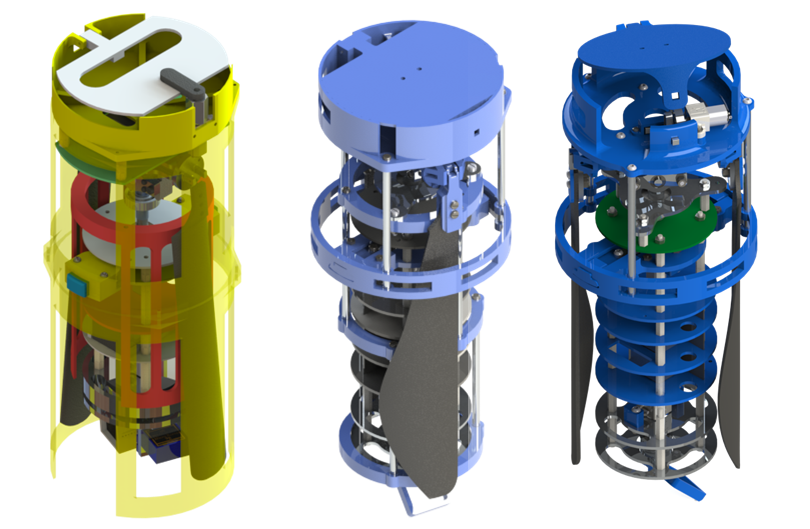
\includegraphics[scale=0.60]{imgmeca/DisenosCansat.png}
	\caption{Dise�os realizados del Cansat siendo el �ltimo (de izquierda a derecha) el seleccionado para construir.}
	\label{img:DisenosCansat}
\end{figure}

\noindent La figura \ref{img:DisenosCansat} es una muestra de que el proceso de dise�o en ingenier�a es inevitablemente iterativo, en d�nde cada iteraci�n representa un mejor entendimiento de los requerimientos y las restricciones del sistema. Dicho entendimiento se refleja en las modificaciones hechas al dise�o en cada iteraci�n.

\newpage
		\subsection{Sistema Central de Manejo del Comportamiento} \label{sistSCMC}
% !TeX encoding = ISO-8859-1

%%%%%%%%%%%%%%%%%%%%%%%%%%%%%%%%%%%%%%%%%%%%%%%%%%%%%%%%%%%%%%%%%%%%%%%%%%%%%%%%%%%%%%%%%%%%%%%%%%%%%%%%%%%
%%%%%%%%%%%%%%%%%%%%%%%%%%%%%%%%%%%%%%%%%%%%%%%%%%%%%%%%%%%%%%%%%%%%%%%%%%%%%%%%%%%%%%%%%%%%%%%%%%%%%%%%%%%
%%%%%%%%%%%%%%%%%%%%%%%%%%%%%%%%%%%%%%%%%%%%%%%%%%%%%%%%%%%%%%%%%%%%%%%%%%%%%%%%%%%%%%%%%%%%%%%%%%%%%%%%%%%


\algblockdefx[SwitchCase]{Switch}{EndSwitch}%
	[1]{\textbf{switch} ( #1 )}%
	{}
	
\algblockdefx[Case]{Case}{Break}%
	[1]{\textbf{case} \textit{#1}:}%
	{\textbf{break}}
	
	
%%%%%%%%%%%%%%%%%%%%%%%%%%%%%%%%%%%%%%%%%%%%%%%%%%%%%%%%%%%%%%%%%%%%%%%%%%%%%%%%%%%%%%%%%%%%%%%%%%%%%%%%%%%
%%%%%%%%%%%%%%%%%%%%%%%%%%%%%%%%%%%%%%%%%%%%%%%%%%%%%%%%%%%%%%%%%%%%%%%%%%%%%%%%%%%%%%%%%%%%%%%%%%%%%%%%%%%
%%%%%%%%%%%%%%%%%%%%%%%%%%%%%%%%%%%%%%%%%%%%%%%%%%%%%%%%%%%%%%%%%%%%%%%%%%%%%%%%%%%%%%%%%%%%%%%%%%%%%%%%%%%	
	
	
	
{\parindent0pt

\indent El SCMC realiza las funciones de adquirir todas las variables internas y externas del CanSat y las env�a al SPD. El SPD entonces procesa dichas variables crudas y las env�a de regreso al SCMC para que �ste tome decisiones de acuerdo a los requerimientos de la misi�n.\\

El SCMC est� estrechamente relacionado con el SPD; ambos comparten componentes f�sicos y recursos de procesamiento. Debido al enfoque funcional, el SCMC y el SPD ser�n abordados de manera independiente; primero se hablar� de las funciones y caracter�sticas de ambos sistemas y despu�s de su construcci�n f�sica.\\

El SCMC se compone de $2$ subistemas: el subsistema de percepci�n ($sS_{1{.}1}-$SP)  y el subsistema de toma de decisiones ($sS_{1{.}2}-$STD).\\

\subsubsection{Subsistema de Percepci�n}

El SP realiza la funci�n $f_{2{.}2}-$\textit{Medir par�metros} y todas las subfunciones respectivas (a excepci�n de que se indique lo contrario). Esta informaci�n se utiliza para la toma de decisiones o para el an�lisis posterior en Tierra.\\

Este sistema est� constituido por todos los sensores del CanSat. Para la selecci�n de los sensores se utilizaron matrices de decisi�n en las que se exponen las caracter�sticas m�s cr�ticas de �stos que fueron tomadas en cuenta para la selecci�n. Estas matrices se muestran al final de la descripci�n del SPD.\\

De acuerdo con la Tabla \ref{tab:Funciones}, la funci�n $2.2$ y todas sus subfunciones, exceptuando la subfunci�n $2.2.1.4$, corresponden al SP de tal modo que a continuaci�n se exponen los sensores seleccionados para realizar dichas funciones.\\

\begin{itemize}
	\item \textbf{GPS:} Usado para adquirir datos de hora UTC, latitud, longitud y altitud sobre el nivel del mar. Este elemento atiende a las funciones $2.2.1.1$ y $2.2.2.6$.
	\item \textbf{Bar�metro:} Usado para medir la presi�n atmosf�rica y de �sta obtener la altura relativa. Este elemento atiende a las funciones $2.2.2.2$ y $2.2.2.6$.
	\item \textbf{Term�metro}: Usado para medir la temperatura del ambiente. Este elemento atiende a la funci�n $2.2.2.1$
	\item \textbf{Giroscopio:} Usado para medir la velocidad angular del CanSat en los tres ejes de un sistema cartesiano. Este elemento atiende a la funci�n $2.2.2.4$.
	\item \textbf{Aceler�metro:} Usado para medir las aceleraciones del CanSat en los tres ejes de un sistema cartesiano. Este elemento atiende a la funci�n $2.2.2.3$.
	\item \textbf{Magnet�metro:} Usado para medir las componentes del campo magn�tico de la Tierra a las que est� sometido el CanSat. Este elemento atiende a la funci�n $2.2.2.5$.
	\item \textbf{Encoder incremental:} Usado para medir la velocidad angular del rotor. Este elemento atiende a la funci�n $2.2.1.3$.
\end{itemize}


\subsubsection{Subsistema de Toma de Decisiones}

El STD se encarga de conferirle al CanSat el comportamiento deseado con base en las variables adquiridas por el SP y procesadas por el SPD.\\

El dise�o de este subsistema fue regido por los eventos de la misi�n, as� como aquellos requeridos por el equipo con el fin de realizar pruebas. Este sistema atiende a las funciones $2.1.4-$\textit{Realizar conteo del n�mero de paquetes enviados} y $2.3-$\textit{Tomar decisiones} con todas sus subfunciones.\\

El comportamiento del CanSat es regido por una m�quina de estados. La m�quina de estados se muestra en la figura \ref{img:StateMachine}\\

\begin{figure}[H]
	\centering
		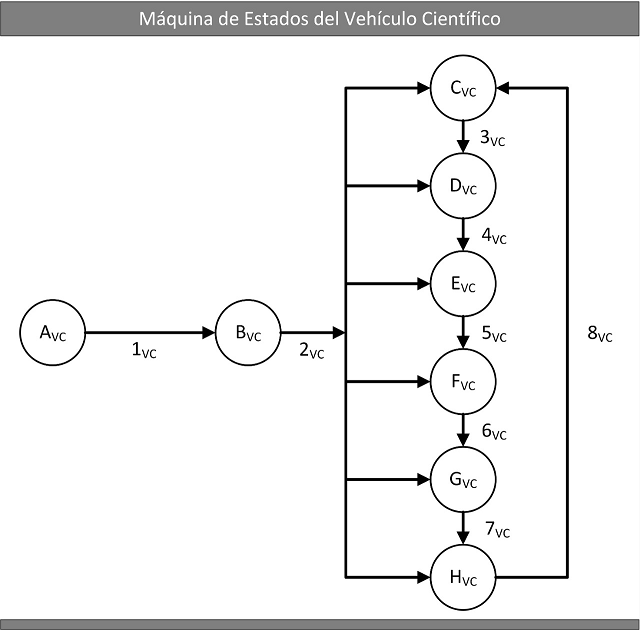
\includegraphics[scale=0.60]{diseniosist/SCMC/StateMachVC}
	\caption{M�quina de estados del veh�culo cient�fico.}
	\label{img:StateMachine}
\end{figure}

La Tabla \ref{EstadosMaquinaVehiculo} describe los estados y la Tabla \ref{TransicionMaquinaVehiculo} describe las condiciones de transici�n entre estados.

\begin{table}[H]
\begin{center}
\caption{Estados de la m�quina de estados del veh�culo cient�fico.}
\label{EstadosMaquinaVehiculo}
\resizebox{14cm}{!}{
\begin{tabular}{p{5cm} p{13cm}}
\multicolumn{2}{c}{}\tabularnewline
\toprule
\multicolumn{1}{c}{\textbf{Evento}} & \multicolumn{1}{c}{\textbf{Descripci�n}}\tabularnewline
\midrule
\tabularnewline

($\text{A}_{\text{VC}}$) Inicio & En este estado se inicializan todos los perif�ricos y sensores del veh�culo cient�fico.\tabularnewline
($\text{B}_{\text{VC}}$) Recuperaci�n del estado anterior & En este estado se lee la memoria no vol�til del veh�culo cient�fico que almacena el �ltimo estado en el que se encontraba el sistema antes de ser reiniciado o encendido. \tabularnewline
($\text{C}_{\text{VC}}$) Diagn�stico del sistema & En este estado se realiza el diagn�stico del sistema, verificando que todos los sensores y perif�ricos respondan como es debido. \tabularnewline
($\text{D}_{\text{VC}}$) Espera de despegue & En este estado el sistema s�lo se encuentra esperando el despegue, no realiza ninguna otra acci�n. En este punto el CanSat debe estar dentro del veh�culo de ascenso.\tabularnewline
($\text{E}_{\text{VC}}$) Ascenso & En este estado el CanSat s�lo realiza lectura, c�mputo y transmisi�n de variables.\tabularnewline
($\text{F}_{\text{VC}}$) Descenso con parac�das & Dentro de este estado el CanSat se encuentra descendiendo con el paraca�das como reductor de velocidad. Se realiza lectura, c�mputo, control y transmisi�n de variables.\tabularnewline
($\text{G}_{\text{VC}}$) Descenso con h�lices & En este estado el veh�culo cient�fico desciende con el sistema de autorrotaci�n. El sistema realiza lectura, c�mputo, control y transmisi�n de variables.\tabularnewline
($\text{H}_{\text{VC}}$) Aterrizaje & En este estado el CanSat se encuentra de nuevo en Tierra. El sistema s�lo activa su dispositivo de localizaci�n.\tabularnewline
\bottomrule
\end{tabular}
}
\end{center}
\vspace{-2.2em}
\end{table}

\begin{table}[H]
\begin{center}
\caption{Condiciones de transici�n de la m�quina de estados del veh�culo cient�fico.}
\label{TransicionMaquinaVehiculo}
\resizebox{14cm}{!}{
\begin{tabular}{ p{3cm} p{13cm} }
\multicolumn{2}{c}{}\tabularnewline
\toprule

\multicolumn{1}{c}{\textbf{Transici�n}} & \multicolumn{1}{c}{\textbf{Descripci�n}}\tabularnewline
\midrule
\tabularnewline

	\centering$\text{1}_{\text{VC}}$ & Todos los sensores se encuentran configurados y operando correctamente.
\tabularnewline
	\centering$\text{2}_{\text{VC}}$ &  En este punto el cambio de estado se realiza de acuerdo con la lectura de la memoria no vol�til del CanSat. El �ltimo estado en el que se haya encontrado el sistema ser� el que se restaurar�. 
\tabularnewline
	\centering$\text{3}_{\text{VC}}$ & El sistema no cambia el estado hasta haber hecho un diagn�stico de los sensores sin reporte de errores. \tabularnewline
	\centering$\text{4}_{\text{VC}}$ & El sistema cambia el estado hasta que se detecte un cambio positivo en la altura de referencia. El cambio debe superar los $10 [m]$ por encima de la altura de referencia.
\tabularnewline
	\centering$\text{5}_{\text{VC}}$ & El sistema cambia el estado hasta que se detecte un cambio negativo en la altura m�xima. El cambio debe superar los $10 [m]$ por debajo de la altura m�xima.
\tabularnewline
	\centering$\text{6}_{\text{VC}}$ & El veh�culo cient�fico cambia el estado hasta encontrarse a una altura de $250 [m]$ por encima de la referencia con una tolerancia de $\pm 10 [m]$.
\tabularnewline
	\centering$\text{7}_{\text{VC}}$ & El estado cambia hasta que el sistema se encuentre de nuevo en la altura de referencia.
\tabularnewline
	\centering$\text{8}_{\text{VC}}$ & El estado cambia hasta que se le env�e un comando de reinicio de estados.
\tabularnewline

\bottomrule
\end{tabular}
}
\end{center}
\end{table}

El Algoritmo \ref{PseudocodigoCanSatP1} corresponde a la m�quina de estados del CanSat. Este algoritmo explica el flujo de actividades dentro del programa del microcontrolador correspondiente al STD.


\begin{algorithm}[H]
\caption{Pseudoc�digo CanSat}
\label{PseudocodigoCanSatP1}
\begin{algorithmic}[1]

\Function{Lectura de sensores}{}
	\State Lee GPS, lee giroscopio, lee aceler�metro, lee magnet�metro, lee presi�n atmosf�rica, lee temperatura, calcula altura actual, calcula marco de referencia actual y realiza control de orientaci�n de la c�mara.
\EndFunction\\

\Function{Transmisi�n y Almacenamiento}{datos de sensores}
	\State Genera la trama de datos
	\State Transmite la trama de datos a estaci�n en Tierra
	\State Guarda la trama de datos en la memoria SD
	\State Guarda el n�mero de trama en la memoria no v�latil
	\State $Conteo Paquetes \gets Conteo Paquetes + 1$
\EndFunction\\

\Procedure{M�quina de vuelo}{}
	\State Configura sensores
	\State Lee memoria no v�latil: estado y n�mero de tramas transmitidas.
	\State Restaura funcionalidades.
	\State $Conteo Actual \gets Conteo Almacenado$
	\State $Estado Actual \gets Estado Almacenado$

	\While{el CanSat est� encendido}
		\Switch{EstadoActual}
		
			 \Case{Diagn�stico del sistema}
			 	\If{ comando de inicio fue recibido }
 				 	\State Prueba comunicaci�n con el GPS
				 	\State Prueba comunicaci�n con la IMU
				 	\State Prueba comunicaci�n con el bar�metro y term�metro
				 	\If{ no errores }
				 		\State Activa secuencia sonora aprobatoria
				 		\State Transmite una se�al aprobatoria en las telecomunicaciones
			 			\State $EstadoActual \gets Espera\enspace del\enspace despegue$
				 	\Else
				 		\State Activa secuencia sonora reprobatoria
				 		\State Transmite una se�al reprobatoria en las telecomunicaciones
				 	\EndIf
			 		\State Almacena \textit{EstadoActual} en memoria no v�latil
			 	\Else
			 		\State Transmite una se�al reprobatoria en las telecomunicaciones
			 	\EndIf
			 \Break	

\algstore{bkbreak}			  
\end{algorithmic}
\end{algorithm}	


\setcounter{algorithm}{0}
\begin{algorithm}[H]
\caption{Pseudoc�digo CanSat (continuaci�n)}
\label{PseudocodigoCanSatP2}
\begin{algorithmic}[1]
\algrestore{bkbreak}

			\Case{Espera del despegue}
			 	\State Ejecuta \textit{\textbf{Lectura de sensores}}
			 	\State Ejecuta \textit{\textbf{Transmisi�n y almacenamiento}}
			 	\If{ $AlturaActual > AlturaReferencia + 10$  }
			 		\State $EstadoActual \gets Ascenso$
			 		\State Almacena \textit{EstadoActual} en memoria no v�latil
			 	\EndIf
			 \Break
			 
			 \Case{Ascenso}
			 	\State Ejecuta \textit{\textbf{Lectura de sensores}}
			 	\State Ejecuta \textit{\textbf{Transmisi�n y almacenamiento}}
			 	\If{ $AlturaActual > AlturaAnterior$ }
				 	\State $AlturaAnterior \gets AlturaActual$
			 	\ElsIf{ $AlturaActual < AlturaAnterior - 10m$ }
					\State Abre paraca�das
			 		\State $EstadoActual \gets Descenso\enspace con\enspace paracaidas$
			 		\State Almacena \textit{EstadoActual} en memoria no v�latil
			 	\EndIf
			 \Break
			 
			 \Case{ Descenso con paraca�das }
			 	\State Ejecuta \textit{\textbf{Lectura de sensores}}
			 	\State Ejecuta \textit{\textbf{Transmisi�n y almacenamiento}}
			 	\If{ $AlturaActual \leq AlturaReferencia+250m$ }
					\State Libera veh�culo cient�fico
			 		\State $EstadoActual \gets Descenso\enspace con\enspace helices$
			 		\State Almacena \textit{EstadoActual} en memoria no v�latil
			 	\EndIf
			 \Break
			 
 			 \Case{ Descenso con h�lices }
			 	\State Ejecuta \textit{\textbf{Lectura de sensores}}
			 	\State Ejecuta \textit{\textbf{Transmisi�n y almacenamiento}}
			 	\If{ $AlturaActual \leq AlturaReferencia+10m$ }
					\State Activa dispositivo de localizaci�n
			 		\State $EstadoActual \gets Aterrizaje$
			 		\State Almacena \textit{EstadoActual} en memoria no v�latil
			 	\EndIf
			 \Break

			\Case{ Aterrizaje }
			 	\State Ejecuta \textit{\textbf{Lectura de sensores}}
			 	\State Ejecuta \textit{\textbf{Transmisi�n y almacenamiento}}
			 	\State Ejecuta secuencia sonora \textit{\textbf{S.O.S.}}
			 	\If{ Comando de reinicio es recibido }
			 		\State $EstadoActual \gets Diagnostico\enspace del\enspace sistema$
			 		\State Almacena \textit{EstadoActual} en memoria no v�latil
				\EndIf
			\Break

		\EndSwitch
	\EndWhile	
\EndProcedure			 
\end{algorithmic}
\end{algorithm}	

Como parte del SCMC se implementaron varios comandos que permiten la ejecuci�n de tareas muy espec�ficas dentro del CanSat, otorg�ndole al usuario control manual sobre el comportamiento del mismo. Cada comando se compone de 10 \textit{bytes} fijos: los campos de `dispositivo' y `tarea' ocupan 1 \textit{byte} cada uno, y el campo de  `valor' ocupa 6 \textit{bytes}. Los dos \textit{bytes} restantes son usados por el caracteres de coma simple (,) que separa los campos.\\

En la Tabla \ref{tab:Commands} se muestran las diferentes combinaciones posibles, con su respectiva explicaci�n.

\begin{table}[H]
\begin{center}
\caption{Lista de comandos.}
\label{tab:Commands}
\resizebox{14cm}{!}{
\begin{tabular}{ p{2cm} p{1cm} p{1.5cm} p{11cm} }
\multicolumn{4}{c}{}\tabularnewline
\toprule
\textbf{Dispositivo} & \textbf{Tarea} & \textbf{Valor} & \textbf{Descripci�n} \tabularnewline
\hline
\multicolumn{4}{c}{}\tabularnewline
\multirow{4}{*}{'M'}
	& 'A' & XXXXXX & Configuraci�n y calibraci�n del aceler�metro.\tabularnewline
	& 'G' & XXXXXX & Configuraci�n y calibraci�n del giroscopio.\tabularnewline
	& 'M' & XXXXXX & Configuraci�n y calibraci�n del magnet�metro\tabularnewline
	& 'S' & XXXXXX & Establecimiento de las referencias de altura y posici�n inicial de la c�mara.\tabularnewline
	\multicolumn{4}{c}{}\tabularnewline
\hline
\multicolumn{4}{c}{}\tabularnewline
\multirow{5}{*}{'B'}
	& 'S' & ------ & Se realiza el dign�stico de los sensores. Si todo es correcto se inicia la misi�n, de lo contrario, el sistema manda la secuencia reprobatoria y se continua en estado de \textit{Diagn�stico}.\tabularnewline
	& 'A' & ------ & Se reinicia todo el sistema. Todas las banderas son limpiadas, las tramas y contadores puestos en cero y el estado es forzado a \textit{Diagn�stico}.\tabularnewline
	& 'R' & ------ & El sistema adquiere una �nica trama de datos y la env�a.\tabularnewline
	& '1' & ------ & El sistema abre las correderas del SLVC.\tabularnewline
	& '2' & ------ & El sistema cierra las correderas del SLVC.\tabularnewline


\bottomrule
\end{tabular}
}
\end{center}
\end{table}

Los comandos con un valor de `M' en el campo de  `dispositivo' son comandos para el SP. Los comandos con un valor de  `B' en el campo de `dispositivo' son comandos para placa principal. Estos comandos pueden ser expandidos ya que cuentan con el campo adicional de `valor', permitiendo as� incrementar la cantidad de los comandos incluyendo valores num�ricos.\\

Finalmente, atendiendo a la funci�n $2.1.4-$\textit{Interactuar con el usuario}, el STD tiene la tarea de informar al usuario si se encuentra o no preparado para la realizaci�n de la misi�n. El sistema informa de cualquier inconveniente utilizando el canal de comunicaci�n con la estaci�n en Tierra y utilizando se�ales auditivas.\\

Para el caso de la comunicaci�n con la estaci�n en Tierra el CanSat responde con 0x4F (letra `O' en ASCII) si todo a sido configurado correctamente y se encuentra listo para realizar la misi�n; o con 0x46 (letra `F' en ASCII) si el sistema encontr� alg�n error durante la inicializaci�n.\\

En el caso de la se�al auditiva el sistema cuenta con una lista de secuencias sonoras que se producen en caso de que suceda alg�n evento espec�fico. Esta lista de secuencias sonoras se muestra en la Tabla \ref{tab:SoundSequence}. Las secuencias se representan por \textit{beeps} cortos y largos, siendo el corto un punto y el largo una l�nea. 


\begin{table}[H]
\begin{center}
\caption{Lista de secuencias sonoras}
\label{tab:SoundSequence}
\resizebox{14cm}{!}{
\begin{tabular}{ p{11cm} >{\centering}p{3cm} }
\multicolumn{2}{c}{}\tabularnewline
\toprule
\textbf{Evento} & \textbf{Secuencia} \tabularnewline
\hline
\multicolumn{2}{c}{}\tabularnewline

Configuraci�n exitosa. Listo para la misi�n. & $\bullet \: \bullet$ \tabularnewline

Error en GPS. & $\bullet \: \bullet \: \bullet \: \bullet$ \tabularnewline

Error en aceler�metro, giroscopio o magnet�metro. & $- \: \bullet \: \bullet \: \bullet$ \tabularnewline

Error en sensor barom�trico y de temperatura. & $\bullet \: - \: \bullet \: \bullet$ \tabularnewline

Altura de referencia no establecida. & $- \: - \: \bullet \: \bullet$ \tabularnewline

El SLVC a�n no tiene la configuraci�n mec�nica correcta, sigue retra�do. & $\bullet \: \bullet \: - \: \bullet$ \tabularnewline

EL control de orientaci�n de la c�mara no se encuentra listo. & $- \: \bullet \: - \: \bullet$ \tabularnewline

No ha sido insertada la memoria SD. & $\bullet \: - \: - \: \bullet$ \tabularnewline

El CanSat ha aterrizado. & $\bullet \: \bullet \: \bullet \: - \: - \: - \: \bullet \: \bullet \: \bullet$ \tabularnewline

\bottomrule
\end{tabular}
}
\end{center}
\end{table}


Las secuencias son �nicas y se generan solamente al momento de realizar un diagn�stico del sistema previo al inicio de la misi�n. La �ltima secuencia, la de aterrizaje, es la �nica que se ejecuta fuera de la etapa de \textit{Diagn�stico} (cuando el CanSat aterriza).


}


\newpage
		\subsection{Sistema de Procesamiento de Datos} \label{sistSPD}
% !TeX encoding = ISO-8859-1

{\parindent0pt

El SPD tiene como objetivo transportar, modificar y almacenar todas las variables del CanSat. Como se dijo anteriormente, el SPD comparte recursos f�sicos y de procesamiento con el SCMC.\\

El SPD se compone de tres subsistemas: subsistema de acondicionamiento de datos ($sS_{2{.}1}-$SAcD), subsistema de almacenamiento de datos ($sS_{2{.}2}-$SAlD) y el subsistema de comunicaci�n interna ($sS_{2{.}3}-$SCI). Al final de esta secci�n se presenta el dise�o electr�nico del SCMC y del SPD de forma detallada.

\subsubsection{Subsistema de Acondicionamiento de Datos}

El SAcD se encarga de adquirir las se�ales crudas provenientes del SP, normalmente presentes en bits menos significativos (\textit{Less Significant Bit}, LSB), y transformarlas en unidades del Sistema Internacional que son m�s entendibles para el usuario y m�s interpretables para la programaci�n. EL SAcD tambi�n se encarga de realizar todas las operaciones matem�ticas para obtener unidades derivadas como la altura calculada a partir de la presi�n atmosf�rica, o la inclinaci�n calculada a partir de valores del aceler�metro y giroscopio. Explicado lo anterior, se proceder� a describir c�mo el dispositivo realiza dichas transformaciones.

\subsubsection*{Transformaciones gen�ricas de unidades}

Estas transformaciones son llevadas a cabo dentro de las rutinas de lecturas de sensores. Las transformaciones gen�ricas dependen �nicamente de la medici�n llevada a cabo en el momento y del factor de conversi�n establecido como constante.\\

Todos los sensores, a excepci�n del GPS, tienen una configuraci�n de sensibilidad. Esta configuraci�n se lleva a cabo al inicializar el sistema y es trabajo del programador determinar cu�l ser� el grado de sensibilidad. La sensibilidad del sensor corresponde al cociente de unidades de medida sobre LSBs, lo que es equivalente a un factor de conversi�n. Los factores de conversi�n se obtienen de la hoja de datos de cada sensor.\\

La f�rmula general para llevar a cabo estas transformaciones es la siguiente:

$$M_T=(M_R)(FC)$$

donde:\\
\null\qquad\qquad$M_T$ es la medida transformada  [unidades]\\
\null\qquad\qquad$M_R$ es la medida cruda [LSBs]\\
\null\qquad\qquad$FC$ es el factor de conversi�n [unidades/LSBs]\\


\subsubsection*{Transformaci�n para la altura}
La altura es una unidad derivada que depende de la presi�n atmosf�rica y de la temperatura adquiridas al momento de la transformaci�n. La siguiente ecuaci�n [?] muestra el c�lculo utilizado para realizar esta transformaci�n (por simplicidad, la temperatura se supuso constante de $15^{\text{o}}\text{C}$):

\begin{equation*}
h = 44330.76923 \left[ 1 - \left( \dfrac{P}{101325} \right)^{0.190263} \right]
\end{equation*}

donde:\\
\null\qquad\qquad$h$ es la altura sobre el lugar de referencia $[m]$\\
\null\qquad\qquad$P$ es la presi�n atmosf�rica medida a la altura $h$ $[Pa]$\\

% [x] -> https://pdfs.semanticscholar.org/59d1/b7706dd7954d7115ae9c8fd7eface3980865.pdf

\subsubsection*{Transformaci�n para la inclinaci�n}

Para el c�lculo de la inclinaci�n del CanSat se sigui� un m�todo que involucra a los datos del giroscopio y aceler�metro en cada eje para realizar un filtro complementario. Dicho c�lculo se basa en un Filtro Extendido de Kalman [?]. En el Algoritmo \ref{MetodoInclinacion} se detalla el pseudoc�digo  para la implementaci�n de este c�lculo.\\

Analizando el Algoritmo \ref{MetodoInclinacion} se observa que el sistema es dependiente del tiempo, de modo que la precisi�n del c�lculo depender� de la velocidad a la cual se realice este algoritmo y de la sensibilidad que tengan los sensores.\\

Debe aclararse que el Algoritmo \ref{MetodoInclinacion} calcula la inclinaci�n para los ejes $pitch$ y $roll$, pero no atiende al c�lculo de $yaw$.\\

Para este �ltimo caso, el �ngulo sobre el eje $yaw$ puede ser obtenido mediante una integraci�n discreta. La ecuaci�n que describe esta integraci�n se presenta a continuaci�n.

\begin{equation*}
yaw = \omega_\text{Z}*\Delta t
\end{equation*}

donde:\\
\null\qquad\qquad$\omega_\text{Z}$ es la velocidad angular medida sobre el eje Z $[deg/s]$\\
\null\qquad\qquad$\Delta t$ es el tiempo entre cada integraci�n $[s]$\\

La precisi�n de estos m�todos depende de la velocidad a la cual el sistema integra la se�al; mientras m�s peque�o sea el tiempo de integraci�n, el error en la se�al de salida ser� menor. Debido a lo anterior, para los c�lculos se utiliz� un tiempo de $10 [ms]$.

\algblockdefx[DoEvery]{DoEvery}{EndDoEvery}%
	[1]{\textbf{while} #1 \textbf{do}}%
	[1]{\textbf{every} #1}

\begin{algorithm}[H]
\caption{Pseudoc�digo para estimaci�n de la inclinaci�n}
\label{MetodoInclinacion}
\begin{algorithmic}[1]

\Ensure Ejes de los sensores sean paralelos o coincidentes
\Ensure Ejes +Z de los sensores se encuentre apuntando hacia arriba
\Require Lecturas del giroscopio y aceler�metro
	
\Procedure{Estimaci�n de la Inclinaci�n}{}
	\State Se normaliza la lectura de gravedad	
	\State Se genera un marco estimado con base en la gravedad
	\State Se calculan los �ngulos con base en el marco estimado
	\DoEvery{El sistema est� encendido}
		\State Se normaliza la lectura de la gravedad
		\If{$Acelerometro_{Z} < 0.1 $} 
		\Comment{Aceler�metro\textsubscript{Z} es la lectura del aceler�metro en el eje Z}
			\State $MarcoReferencia_{G} \gets MarcoReferencia_{E}$
			\Comment{MarcoReferencia\textsubscript{G} es el marco de referencia del giroscopio y MarcoReferencia\textsubscript{E} es el marco de referencia estimado}
		\Else
			\State Calcula MarcoReferencia\textsubscript{G} con los datos actuales
		\EndIf
		\State $MarcoReferencia_{E} \gets MarcoReferencia_{G} \cup MarcoReferencia_{A}$
		\Comment{MarcoReferencia\textsubscript{A} es el marco de referencia del Aceler�metro}
		\State $MarcoReferencia_{E} \gets MarcoReferencia_{E} Normalizado$
		\State Calcula $pitch$ y $roll$
	\EndDoEvery{n milisegundos}
\EndProcedure
\end{algorithmic}
\end{algorithm}


% [Z] -> https://www.instructables.com/id/Accelerometer-Gyro-Tutorial/

\subsubsection{Subsistema de Almacenamiento de Datos}

Este subsistema se encarga de almacenar las tramas de datos ya procesados, as� como cualquier otra variable de inter�s para el correcto funcionamiento del sistema (estado actual, valores de calibraci�n y condiciones iniciales). Es responsabilidad de este subsistema el llevar a cabo el almacenamiento y recuperaci�n de la informaci�n antes y despu�s de un reinicio.\\

El CanSat lleva a bordo una tarjeta SD donde se guardan las tramas de datos enviadas a la estaci�n en Tierra. Tambi�n, el CanSat posee una memoria no vol�til en donde se almacenan los valores de configuraci�n y calibraci�n (valores de calibraci�n de los sensores, alturas de referencia, tiempo de misi�n, n�mero de paquete y estado actual).


\subsubsection{Subsistema de Comunicaci�n Interna}

Este subsistema lleva acabo todas las tareas de comunicaci�n entre los diferentes dispositivos. Dentro de este subsistema se definen los diferentes protocolos a usar, as� como los medios para realizar la comunicaci�n entre elementos.\\

Debido a la gran cantidad de perif�ricos que se utilizan, as� como a la poca disponibilidad de espacio, se opt� por la utilizaci�n de protocolos de comunicaci�n de tipo serial ya que no requieren muchos cables. Algunos protocolos con estas caracter�sticas son los protocolos de comunicaci�n I2C, SPI y RS232.\\

El protocolo RS232 a 115200 baudios se utiliz� para la comunicaci�n entre la placa principal y el SP. Por otra parte, la mayor�a de los sensores en el mercado utilizan los protocolos I2C y SPI. Sin embargo, se utiliz� el protocolo I2C pues requiere s�lo 2 l�neas de comunicaci�n independientemente de la cantidad de sensores usados.\\

\subsubsection{Desarrollo Electr�nico}

En esta secci�n se muestran los componentes electr�nicos utilizados por el SCMC y el SPD. Al final de esta secci�n se muestran los circuitos esquem�tico.\\

El primer componente seleccionado fue la unidad de almacenamiento. Este elemento debe contar con las caracter�sticas de facilidad de uso y extracci�n, alta capacidad de almacenamiento, tama�o peque�o y poca masa. Una tarjeta microSD cumple con estas caracter�sticas. Ahora, la Tabla \ref{tab:sensores} enlista los sensores utilizados en el SP para medir los par�metros internos y externos del CanSat.\\

\begin{table}[H]
\begin{center}
\caption{Sensores utilizados en el SP.}
\label{tab:sensores}
\resizebox{\textwidth}{!}{
\begin{tabular}{
	c>{\centering}
	p{1.8cm}>{\centering}
	p{1.8cm}>{\centering}
	p{1.8cm}>{\centering}
	p{1.8cm}>{\centering}
	p{1.8cm}>{\centering}
	p{1.8cm}>{\centering}
	p{1.8cm}>{\centering}
	p{1.8cm}>{\centering}
	p{1.8cm}
}
\multicolumn{10}{c}{}\tabularnewline
\toprule 
\multirow{3}{*}{\textbf{Modelo}} & \multicolumn{9}{c}{\textbf{Criterios}}\tabularnewline
\cmidrule{2-10} 
	& \textbf{Sensor}
	& \textbf{Voltaje de Operaci�n}
	& \textbf{Cte. de Operaci�n}
	& \textbf{Canales}
	& \textbf{Tasa de Actualizaci�n}
	& \textbf{Cold Start}
	& \textbf{Warm Start}
	& \textbf{Hot Start}
	& \textbf{Soporte Multi Canal}
	\tabularnewline
	
	& 
	& {[}V{]}
	& {[}mA{]}
	& 
	& {[}Hz{]}
	& {[}s{]}
	& {[}s{]}
	& {[}s{]}
	& 
	\tabularnewline
	
\multicolumn{10}{c}{}\tabularnewline	

	  BN-180
	& GPS
	& 2.8-6
	& 50
	& 72
	& 10
	& 26
	& 25
	& 1
	& No
	\tabularnewline

%	  NEO M8N
%	& 1.6-3.6
%	& 67
%	& 72
%	& 10
%	& 29
%	& 26
%	& 1
%	& S�
%	& 30
%	\tabularnewline
	
%	  NEO M6N
%	& 1.6-3
%	& 67
%	& 56
%	& 10
%	& 30
%	& 28
%	& 1
%	& No
%	& 20
%	\tabularnewline

		
\bottomrule
\end{tabular}
}
\end{center}
\end{table}



\begin{center}
\resizebox{\textwidth}{!}{
\begin{tabular}{
	c>{\centering}
	p{1.8cm}>{\centering}
	p{1.8cm}>{\centering}
	p{1.8cm}>{\centering}
	p{1.8cm}>{\centering}
	p{1.8cm}>{\centering}
	p{1.8cm}>{\centering}
	p{1.8cm}>{\centering}
	p{1.8cm}>{\centering}
	p{1.8cm}
}
\multicolumn{10}{c}{}\tabularnewline
\toprule 
\multirow{3}{*}{\textbf{Modelo}} & \multicolumn{9}{c}{\textbf{Criterios}}\tabularnewline
\cmidrule{2-10} 
	& \textbf{Sensor}
	& \textbf{Voltaje de Operaci�n}
	& \textbf{Cte. de Operaci�n}
	& \textbf{Aceler�metro}
	& \textbf{}
	& \textbf{Giroscopio}
	& \textbf{}
	& \textbf{Magnet�metro}
	& \textbf{}
	\tabularnewline
	
	&
	& {[}V{]}
	& {[}mA{]}
	& 
	&
	&
	&
	&
	& 
	\tabularnewline
	
\multicolumn{10}{c}{}\tabularnewline	

	  ICM20948
	& IMU
	& 1.7-3.6
	& 4
	& 2,4,8,16 {[}g{]}
	& 16 bits
	& 250,500,1000,2000 {[}dps{]} 
	& 16 bits
	& 1900 {[}uT{]}
	& 16 bits
	\tabularnewline
		
\bottomrule
\end{tabular}
}
\end{center}


\begin{center}
\resizebox{\textwidth}{!}{
\begin{tabular}{
	c>{\centering}
	p{2cm}>{\centering}
	p{2cm}>{\centering}
	p{2cm}>{\centering}
	p{2cm}>{\centering}
	p{2cm}>{\centering}
	p{2cm}>{\centering}
	p{2cm}
}
\multicolumn{8}{c}{}\tabularnewline
\toprule 
\multirow{3}{*}{\textbf{Modelo}} & \multicolumn{7}{c}{\textbf{Criterios}}\tabularnewline
\cmidrule{2-8}
	& \textbf{Sensor}
	& \textbf{Voltaje de Operaci�n}
	& \textbf{Cte. de Operaci�n}
	& \textbf{Rango Presi�n}
	& \textbf{Resoluci�n Presi�n}
	& \textbf{Rango Temperatura}
	& \textbf{Resoluci�n Temperatura}
	\tabularnewline

	&
	& {[}V{]}
	& {[}uA{]}
	& {[}hPa{]}
	& {[}hPa{]}
	& {[}C{]}
	& {[}C{]}
	\tabularnewline
	
\multicolumn{8}{c}{}\tabularnewline	

%	  LPS22HBT
%	& 1.7-3.6
%	& 15
%	& 260-1260
%	& 0.1
%	& 0-65
%	& 0.01
%	& 3.43
%	\tabularnewline
	
	  DPS310
	& Presi�n y Temperatura
	& 1.7-3.6
	& 75
	& 300-1200
	& 0.005
	& 0-65
	& 0.01
	\tabularnewline
	
%	  BMP280
%	& 1.7-3.6
%	& 1120 
%	& 300-1100
%	& 0.12
%	& 0-65
%	& 0.01
%	& 3.99
%	\tabularnewline

		
\bottomrule
\end{tabular}
}
\end{center}


Finalmente, se hablar� de las unidades l�gicas de control. El SP debe gestionar todos los componente anteriores de modo que debe contar con una unidad l�gica que permita realizar tales tareas, es por ello que se contempla un microcontrolador de bajo consumo y peque�as dimensiones, pero con buena capacidad de c�mputo y m�ltiples puertos de comunicaci�n. Por otro lado, tambi�n se tiene la unidad l�gica de la placa principal, el cual debe tener una alta capacidad de control de perif�ricos y por ende gran capacidad de manejo de informaci�n que se traduce en altas velocidades de c�mputo. La Tabla \ref{tab:Micro} muestra los dos microcontroladores selccionados as� como algunas de sus caracter�sticas principales.\\

\begin{table}[H]
\begin{center}
\caption{Microcontroladores del CanSat.}
\label{tab:Micro}
\resizebox{\textwidth}{!}{
\begin{threeparttable}
\begin{tabular}{c>{\centering}p{2cm}>{\centering}p{2cm}>{\centering}p{1.5cm}>{\centering}p{2cm}>{\centering}p{3cm}>{\centering}p{2cm}>{\centering}p{1.5cm}}
\multicolumn{8}{c}{}\tabularnewline
\toprule 
\multirow{2}{*}{Modelos} & \multicolumn{7}{c}{Criterios}\tabularnewline
\cmidrule{2-8} 
 & Voltaje de operaci�n {[}V{]} & Cte. de operaci�n {[}mA{]} & SRAM {[}kB{]} & Velocidad de operci�n {[}MHz{]} & Interfaces de comunicaci�n & Arquitectura & Precio {[}USD{]}\tabularnewline
%\multicolumn{1}{c}{PIC18F45K40} & 

%1.8 - 5.5 & 

%9 & 

%2 & 

%64 & SPI(x2) \& USART(x2) \& I2C(x2) & 

%8 - bits & 

%3\tabularnewline
\multicolumn{1}{c}{STM32L432KC} & 

1.6 - 3.3  & 

\textasciitilde 6\tnote{1} & 

64 & 

80 & SPI(x4) \& USART(x5) \& I2C(x3) & 32 - bits & 

7.22\tabularnewline
%ATMega328P & 

%1.8 - 5.5  & \textasciitilde 3 & 

%2 & 

%20 & SPI(x1) \& USART(x1) \& I2C(x1) & 

%8 - bits & 

%2.5\tabularnewline
STM32F446RE & 

1.6 - 3.3 & 

83\tnote{1} & 

128 & 

180 & SPI(x4) \& USART(x6) \& I2C(x4) & 

32 - bits & 

11.2\tabularnewline
\bottomrule
\end{tabular}
\begin{tablenotes}
	\item[1] Haciendo uso de la m�xima frecuencia de operaci�n y usando todos los perif�ricos disponibles.
\end{tablenotes}
\end{threeparttable}
}
\end{center}
\end{table}



De acuerdo a los criterios de selecci�n y a las funciones deseadas, el microcontrolador seleccionado para el SP es el STM32L432KC de STMicroelectronics\textregistered, debido a su bajo consumo de corriente en relaci�n a sus perif�ricos y velocidad de operaci�n. Adem�s, en el caso de la placa principal, el microcontrolador STM32F446RE fue seleccionado, las razones fueron su alta velocidad de c�mputo, cantidad de pines para el manejo de perif�ricos, alta capacidad de memoria embebida, entre otros.\\

Por �ltimo, en las figuras \ref{img:EsquematicoMS} y \ref{img:EsquematicoPP} se muestran los circuitos esquem�ticos del SP y del sistema completo, respectivamente.\\

\begin{figure}[H]
	\centering
		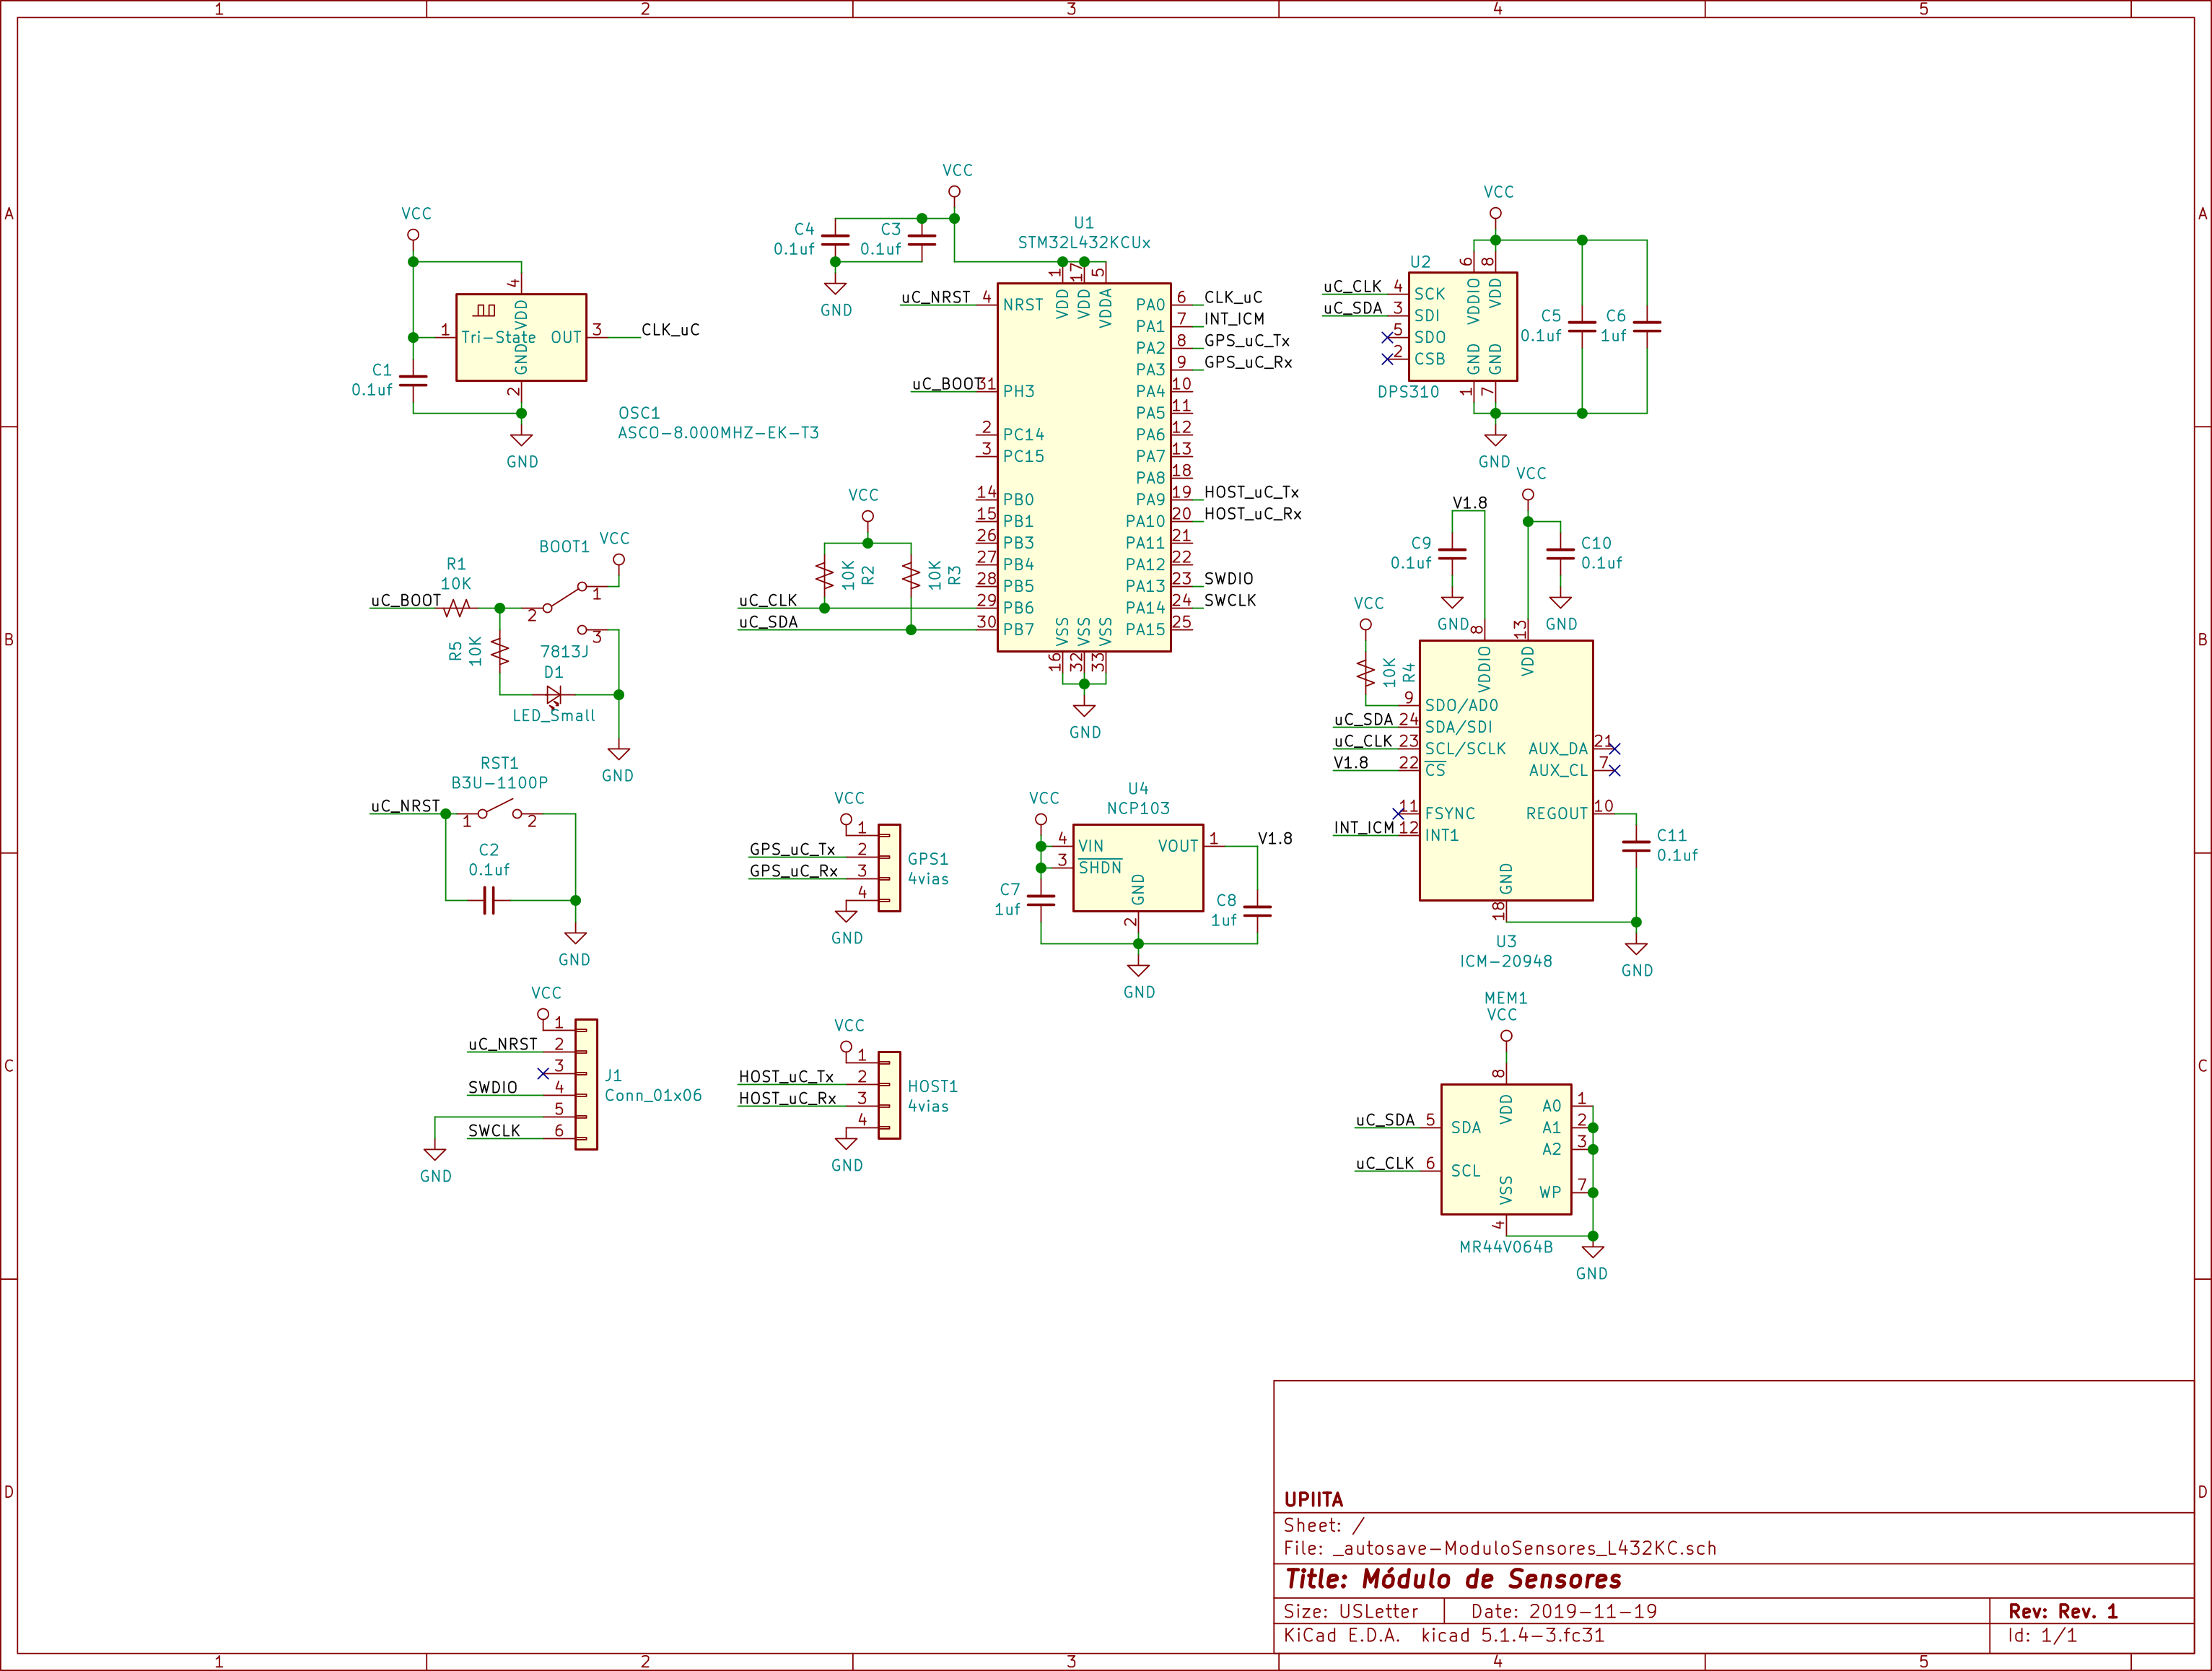
\includegraphics[angle=-90,scale=0.75]{diseniosist/SPD/Modulo_Sensores}
	\caption{Circuito esquem�tico del subsistema de percepci�n (m�dulo de sensores)}
	\label{img:EsquematicoMS}
\end{figure}

\begin{figure}[H]
	\centering
		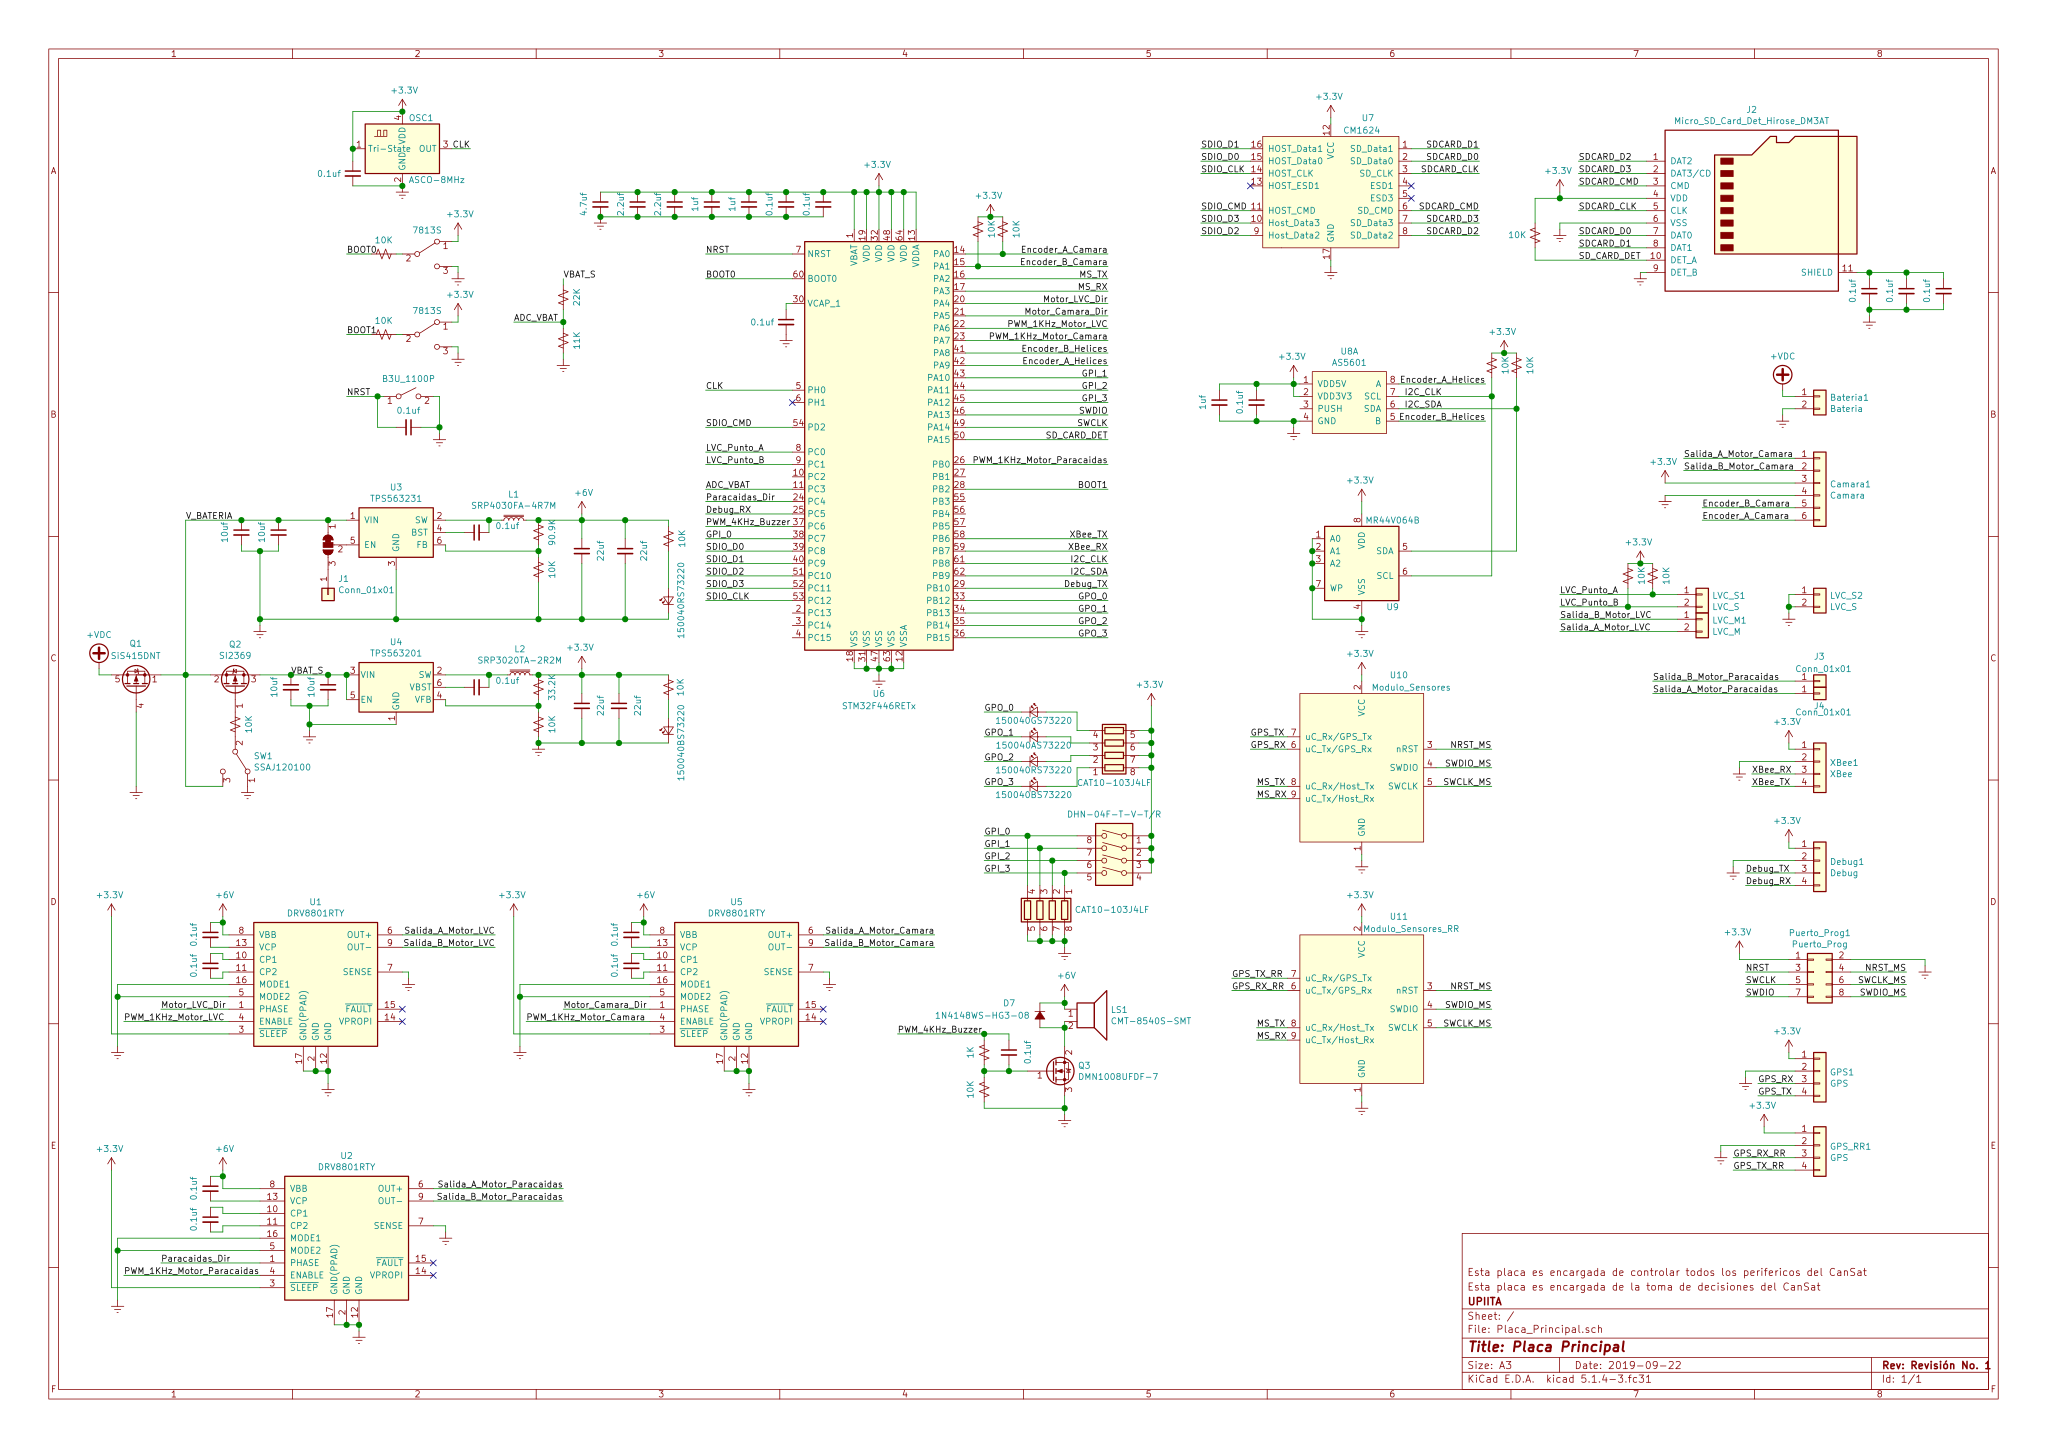
\includegraphics[angle=90,scale=0.5]{diseniosist/SPD/Placa_Principal}
	\caption{Circuito esquem�tico de la placa principal}
	\label{img:EsquematicoPP}
\end{figure}

}


\newpage
		\subsection{Sistema de Reducci�n de Velocidad de Descenso} \label{sistSRVD}
% !TeX encoding = ISO-8859-1

{\parindent0pt

\subsubsection{Subsistema de Reducci�n de Velocidad por Paraca�das}
La velocidad de descenso de cualquier cuerpo equipado con un paraca�das depende de la fuerza de arrastre que desarrolla el paraca�das para contrarrestar la fuerza gravitacional que resulta de la masa del cuerpo. La magnitud de la fuerza de arrastre depende de la presi�n din�mica, la cual est� en funci�n de la velocidad y la densidad del aire, que a su vez dependen de la altitud y de la temperatura, el di�metro del docel del paraca�das y el coeficiente de arrastre.\\

Considerando la segunda ley de Newton se puede establecer un modelo matem�tico simplificado que relaciona las fuerzas que act�an en el CanSat mientras desciende con paraca�das. Para desarrollar este modelo se tomaron varias consideraciones: 1) el sistema consiste en un paraca�das sim�trico conectado r�gidamente por un conector de longitud fija y 2) se considera s�lo un grado de libertad, haciendo referencia a la ca�da libre del CanSat. El modelo matem�tico simplificado del movimiento del paraca�as se presenta en la ecuaci�n \eqref{eq:Parachute1}:
% y el diagrama de cuerpo libre se muestra en la figura \ref{img:SRVDparachute_dcl}.

\begin{align}
\label{eq:Parachute1}
\overrightarrow{\text{W}}_{\text{C}} - \overrightarrow{\text{F}}_{\text{R}} - \overrightarrow{\text{F}}_{\text{D}} = m_c a
\end{align}

donde:\\
\null\qquad\qquad$\overrightarrow{\text{W}}_{\text{C}}$ es la fuerza gravitacional que resulta de la masa del CanSat $[N]$.\\
\null\qquad\qquad$\overrightarrow{\text{F}}_{\text{R}}$ es la fuerza de arrastre producida por la geometr�a del CanSat $[N]$.\\
\null\qquad\qquad$\overrightarrow{\text{F}}_{\text{D}}$ es la fuerza de arrastre producida por el paraca�das $[N]$.\\
\null\qquad\qquad$m_c$ es la masa del CanSat $[Kg]$.\\
\null\qquad\qquad$a$ es la aceleraci�n del CanSat $[m/s^2]$.\\

Adem�s:\\
\null\qquad\qquad$\frac{dv}{dt}=a$\\
\null\qquad\qquad$\overrightarrow{\text{W}}_{\text{C}}=m_c g$ (donde $g=9.81 [m/s^2]$).\\
\null\qquad\qquad$\overrightarrow{\text{F}}_{\text{R}}=k(v) C_c S_c$\\
\null\qquad\qquad$\overrightarrow{\text{F}}_{\text{D}}=k(v) C_d S_p$\\
\null\qquad\qquad$k(v) = (0.5 v^2 \rho)/(m_c)$\\
\null\qquad\qquad$\rho=1.225 [kg/m^3]$ es la densidad del aire.\\
\null\qquad\qquad$C_d$ es el coeficiente de arrastre del paraca�das $[adimensional]$.\\
\null\qquad\qquad$C_c$ es el coeficiente de arrastre de la geometr�a del CanSat $[adimensional]$.\\
\null\qquad\qquad$S_p$ es la superficie efectiva del paraca�das $[m^2]$.\\
\null\qquad\qquad$S_c$ es la superficie efectiva del CanSat $[m^2]$.\\

Si la ecuaci�n \eqref{eq:Parachute1} se resuelve para $\frac{dv}{dt}$ se obtiene la ecuaci�n \eqref{eq:Parachute2}:

\begin{align}
\label{eq:Parachute2}
\frac{dv}{dt} = (0.5 v^2 \rho/m_c)(C_d S_p + C_c S_c) + g
\end{align}

Con la ecuaci�n \eqref{eq:Parachute2} se pueden determinar las dimensiones del paraca�das. Para esto, se tomaron en cuenta dos consideraciones: 1) la aportaci�n de la fuerza de rozamiento del CanSat $\overrightarrow{\text{F}_{\text{R}}}$ es mucho menor a la fuerza de arrastre producida por el paraca�das $\overrightarrow{\text{F}_{\text{D}}}$ y, por lo tanto, se puede omitir para una primera aproximaci�n de las dimensiones del paraca�das; y 2) el c�lculo se realiza en el r�gimen estacionario, una vez que la velocidad de descenso ha alcanzado su valor l�mite, por lo tanto, $\frac{dv}{dt} = 0$. As�, la ecuaci�n \eqref{eq:Parachute2} se resuelve para $S_p$, quedando la ecuaci�n \eqref{eq:Parachute3}.

%\begin{figure}[H]
%	\begin{center}
%		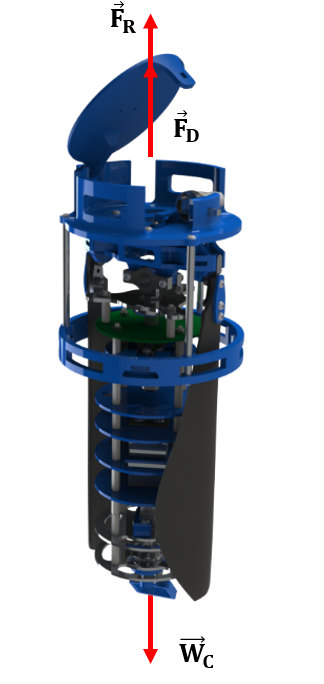
\includegraphics[scale=0.25]{imgmeca/Simplificadoparacaidas.png}  
%		\caption{Fuerzas que act�an sobre el CanSat durante el descenso por paraca�das.}
%		\label{img:SRVDparachute_dcl}
%	\end{center}
%\end{figure}

\begin{align}
\label{eq:Parachute3}
S_p = \frac{2 m_c g}{\rho v^2 C_d}
\end{align}

De \cite{} se obtiene que el coficiente de arrastre $C_d$ de un paraca�das hemisf�rico es de $0.66$. Adem�s, cabe se�alar que para los c�lculos se va a considerar un velocidad constante de descenso $v = 17 [m/s]$ con la finalidad de dar un margen de tolerancia en los resultados. Con estos valores se obtiene un valor $S_p = 0.04282 [m^2]$, que equivalen a un radio de paraca�das $r_p = 0.1167 [m]$.\\

Para resolver la ecuaci�n \eqref{eq:Parachute2} se tiene que para el coeficiente de arrastre $C_c$ en \cite{} se da una gr�fica en la que se tienen que interpolar los datos de la relaci�n entre la longitud del CanSat $l_c$ y el di�metro que posee $d_c$, $l_c/dc$, y el n�mero de Reynolds que se produce durante la velocidad de descenso por medio del paraca�das. Tomando en cuenta todo lo anterior se tiene que $C_c = 0.80$. El �rea efectiva del CanSat para un di�metro de $0.105 [m]$ es de $S_c = 0.008659 [m^2]$. Tomando una masa l�mite para el CanSat de $510 [g]$ la figura \ref{img:res_parachute} muestra la gr�fica de la velocidad que te�ricamente alcanzar�a el CanSat en su descenso con paraca�das.\\

En la figura \ref{img:res_parachute} se muestra que la velocidad de descenso del CanSat con paraca�das tiende a una valor de $15.2358 [m/s]$, que est� dentro de los l�mites establecidos en los requerimientos.\\

Con estos datos se dise�� el compartimento del paraca�das ubicado en la parte superior del contenedor. Este compartimento tiene la capacidad de alojar el paraca�das y tiene un mecanismo que permite que el paraca�das se despliegue. Los elementos que conforman este compartimiento se muestran en la figura \ref{img:Compartimientoparacaidas}. Como elementos de sujeci�n se utilizaron tornillos M3 y M2 de diferentes longitudes y tuercas de bloqueo con inserto de nylon.

\begin{figure}[H]
	\begin{center}
		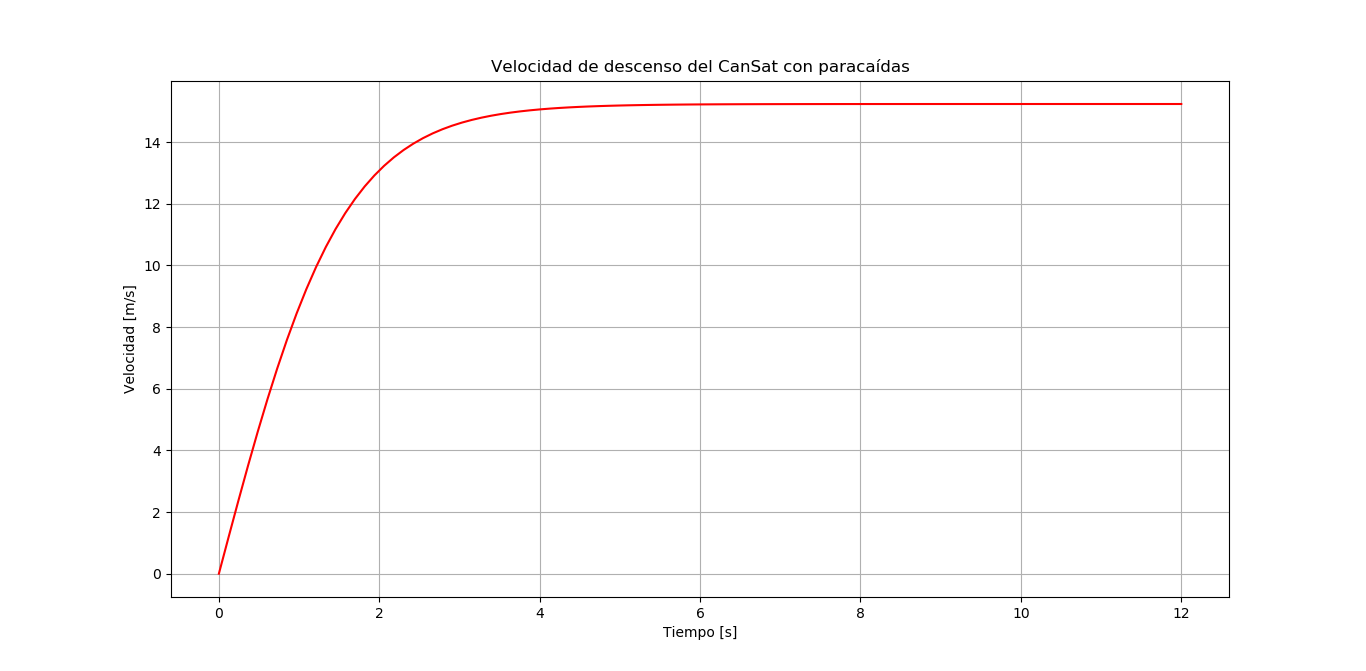
\includegraphics[scale=0.40]{imgmeca/parachute_descent.png}  
		\caption{Estimaci�n de la velocidad de descenso del CanSat con paraca�das.}
		\label{img:res_parachute}
	\end{center}
\end{figure}


\begin{figure}[H]
	\begin{center}
		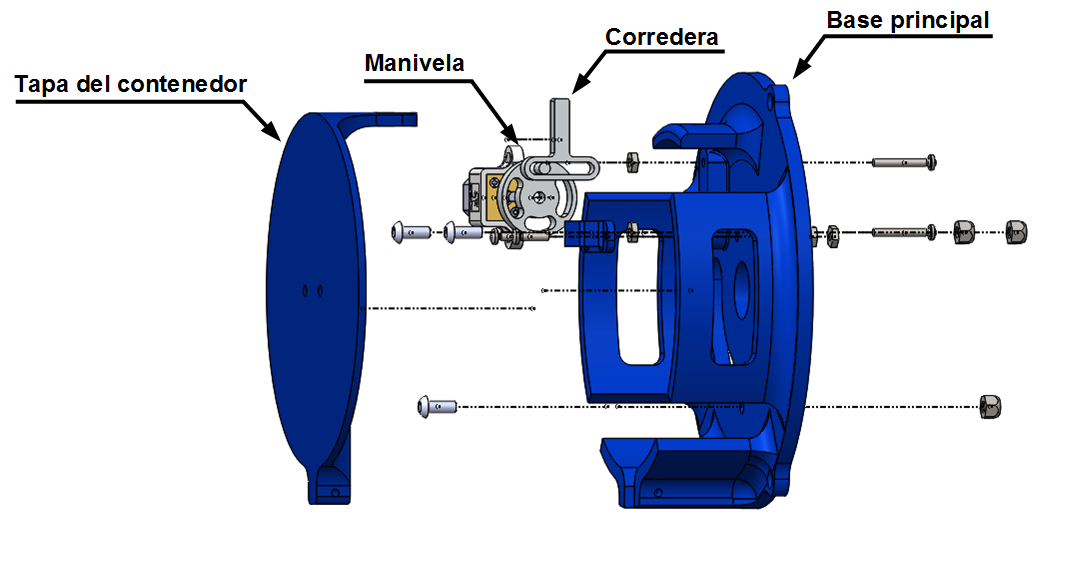
\includegraphics[scale=0.40]{imgmeca/SistemaParacaidas.png}
		\caption{Componentes que conforman la parte superior del contenedor. \label{img:Compartimientoparacaidas}}
	\end{center}
\end{figure}

El paraca�das se encontrar� alojado adentro de la parte superior del contenedor y va a estar sujetado a tres puntos de anclaje, los cuales se encuentra a una inclinaci�n de $120 ^{\circ}$ y a una separaci�n de $60 [mm]$ del centro. La geometr�a de la base principal se dise�� con la finlidad de que las aperturas en los costados, as� como las que se encuentran en la parte inferior, ayuden a la expulsi�n e inflado del paraca�das.\\

En la figura \ref{img:aperturaparachute} se muestra la secuencia de activaci�n para la apertura del paraca�das. En el cuadro de la izquierda de la figura \ref{img:aperturaparachute} se muestra el estado de reposo, donde O representa el centro de la geometria y $x_0$ es la posci�n inicial de la corredera. En este estado el mecanismo de apertura permanece sin movimiento durante el ascenso del CanSat. Una vez que el CanSat es liberado y ha ca�do $10 [m]$ con respecto de la altura de apogeo, se pasa al estado de transici�n en el cual la manivela realiza un giro a consecuencia del par proporcionado por el motor. Lo anterior permite que la corredera se desplace de la posici�n inicial $x_0$ a una posici�n $x_i$. Cuando la corredera ha abandonado la pared de la tapa del contenedor, �sta misma, por acci�n del viento, gira y permite la expulsi�n del paraca�das (cuadro derecho de la figura \ref{img:aperturaparachute}). En el estado final, cuando la corredera se encuentra en $x_i$, la tapa del paraca�das ha girado totalmente. El motor deja de suministrar el torque a la manivela y, por acci�n de un interruptor de final de carrera, se le deja de suministrar voltage al motor.\\

\begin{figure}[H]
	\begin{center}
		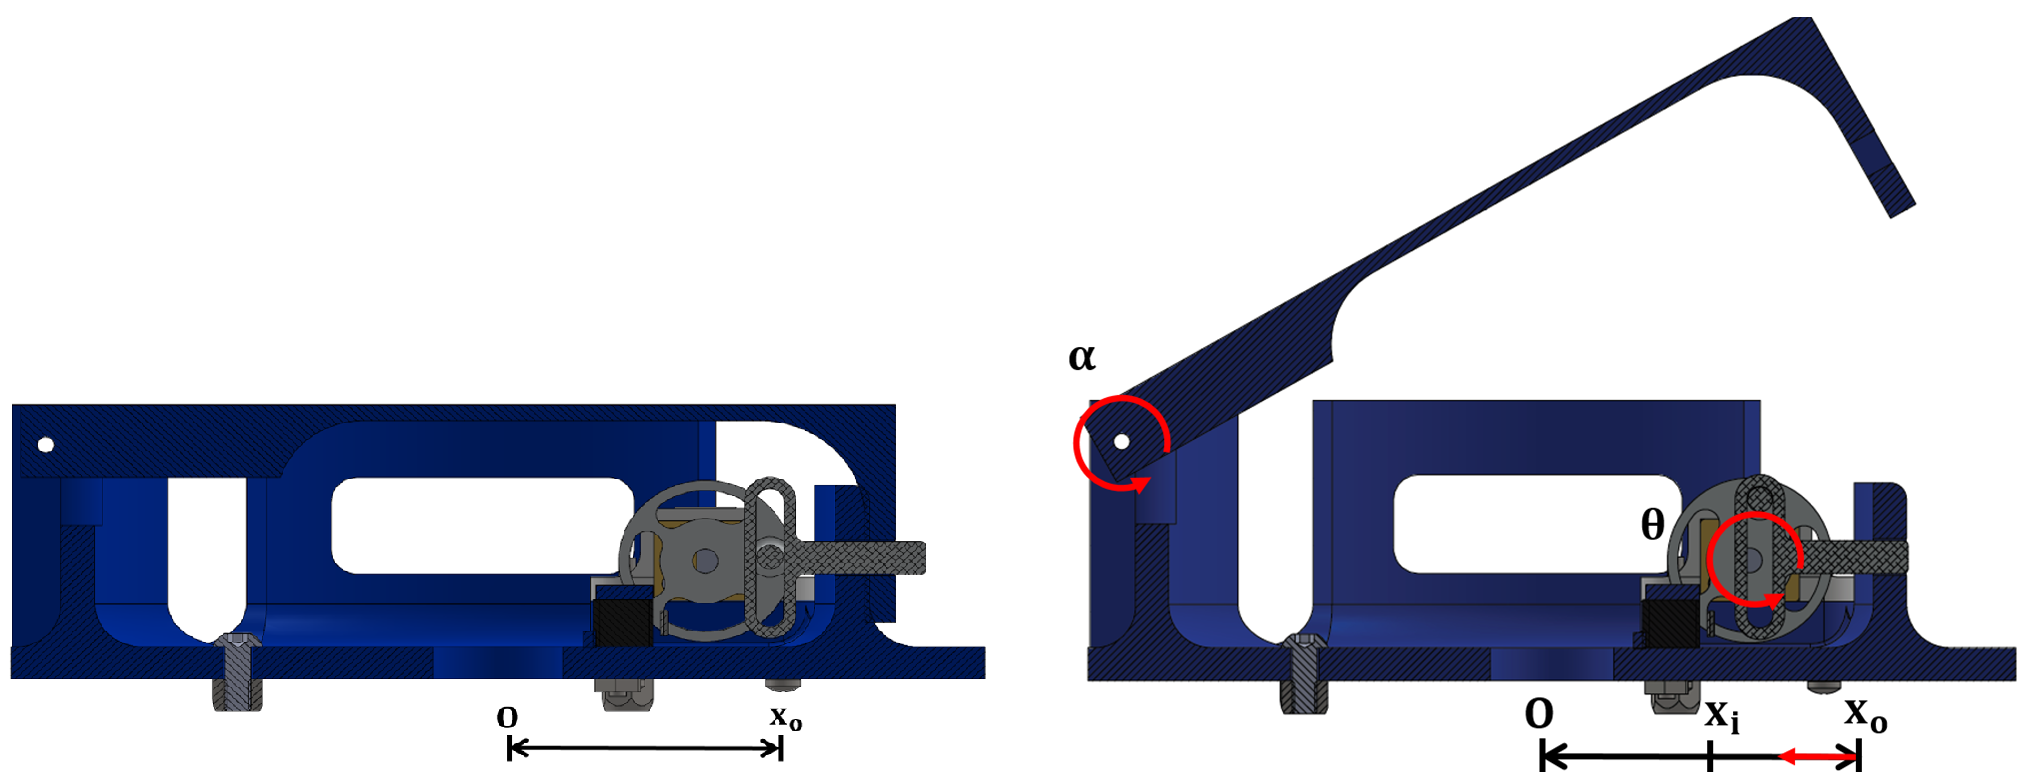
\includegraphics[scale=0.25]{imgmeca/parachute_secuencia.png}
		\caption{Secuencia de activaci�n del mecanismo de apertura del paraca�das. \label{img:aperturaparachute}}
	\end{center}
\end{figure}

\subsubsection*{Selecci�n de materiales}
Tomando como base el proceso de selecci�n de materiales propuesto por Ashby en \cite{}, la Tabla \ref{Alex3} muestra la traducci�n de los requerimientos a especificaciones de material.\\

La manivela y la corredera son componentes cr�ticos del mecanismo de apertura del paraca�das ya que son los que estar�n sometidos a esfuerzos durante el ascenso del CanSat. Por ese motivo, se opt� por fabricar esas piezas de aluminio.\\

Para la selecci�n de la aleaci�n de aluminio a utilizar se consideraron varios criterios, entre ellos las propiedades mec�nicas, la disponibilidad en el mercado nacional, el precio y la facilidad de maquinado. Ejemplo de estas aleaciones son las que  pertenecen a la serie AA 1xxx, AA 6xxx y AA 7xxx. En la Tabla \ref{tab:aleaciones} se muestran algunas de las propiedades mec�nicas de las aleaciones de aluminio m�s comerciales.\\

De acuerdo con los datos presentados en la Tabla \ref{tab:aleaciones} se seleccion� la aleaci�n AA 6061 por ser la que posee la densidad m�s baja y un m�dulo de elasticidad y maquinabilida aceptables.

\begin{table}[H]
	\begin{center}
		\caption{Traducci�n de requerimientos a especificaciones de materiales del SRVD.}
		\label{Alex3}
		\resizebox{12cm}{!}{
			\begin{tabular}{m{4cm}p{10cm}}
				\multicolumn{2}{c}{}\tabularnewline
				\toprule
				\textbf{Funciones} & Liberar el paraca�das.\tabularnewline
				\textbf{Restricciones} &
				- Temperatura de trabajo: debe soportar temperaturas de hasta 60 [� C].\newline
				- Resistencia: debe soportar el peso del CanSat durante el descenso.\newline
				- Rigidez: no debe sufrir grandes deformaciones al momento del ascenso.\newline
				- Bajo coeficiente de fricci�n.
				\tabularnewline
				\textbf{Objetivos} & Minimizar masa.\tabularnewline
				\textbf{Variables libres} &
				- Forma de los componentes del mecanismo.\newline
				- Selecci�n del material.
				\tabularnewline
				\bottomrule
			\end{tabular}
		}
	\end{center}
\end{table}


\begin{table}[H]
	\begin{center}
		\caption{Propiedades de las aleaciones de aluminio consideradas.\label{tab:aleaciones}}
		\resizebox{14cm}{!}{
			\begin{tabular}{>{\centering}p{2cm}>{\centering}p{3cm}>{\centering}p{3.5cm}>{\centering}p{3cm}>{\centering}p{3cm}>{\centering}p{3cm}}
				\multicolumn{6}{c}{}\tabularnewline
				\toprule
				\textbf{Aleaci�n} & \textbf{Densidad $\left[ \text{g} \cdot \text{cm}^{-3} \right]$} & \textbf{M�dulo de elasticidad $\left[ \text{GPa} \right]$} & \textbf{Maquinibilidad} & \textbf{Dureza Brinell $\left[ \text{HB} \right]$}  & \textbf{Disponibilidad} \tabularnewline \hline \tabularnewline
				  
				AA 1100 & 2.71 & 68.0 & Pobre & 32 & Nacional\tabularnewline
				AA 6061 & 2.70 & 68.9 & Aceptable & 60 & Nacional \tabularnewline
				AA 7075 & 2.81 & 71.1 & BUena & 150 & Nacional\tabularnewline
				 
				\bottomrule
			\end{tabular}
		}
	\end{center}
\end{table}


\begin{table}[H]
	\begin{center}
		\caption{Propiedades del ABS.}
		\label{ABS}
		\resizebox{12cm}{!}{
			\begin{tabular}{>{\centering}p{3cm}>{\centering}p{2cm}>{\centering}p{2cm}>{\centering}p{2cm}>{\centering}p{4cm}}
				\multicolumn{5}{c}{}\tabularnewline
				\toprule
				\textbf{Material} & \textbf{Densidad [kg/$\text{m}^{3}$]} & \textbf{M�dulo de elasticidad [GPa]} & \textbf{Esfuerzo de cedencia [MPa]} & \textbf{Temperatura de trabajo m�xima [� C]}\tabularnewline \hline \tabularnewline
				
				ABS  & 1050 & 1.68 & 39 & 85\tabularnewline
%				Aluminio 6061 & 2730 & 66.6 & 240 & 130\tabularnewline
				
				\bottomrule
			\end{tabular}
		}
	\end{center}
\end{table}

Para el caso de la base principal y la tapa del contenedor se necesita poca fricci�n y ligereza. Fabricar de aluminio estas piezas representar�a mucha masa para el CanSat por lo que se propone el uso del la impresi�n 3D con ABS (\textit{Acrylonitrile Butadiene Styrene}, por sus siglas en ingl�s.) junto con un tratamiento con vapor de acetona para eliminar la mayor cantidad de imperfecciones producidas por el proceso de deposici�n de material y as� reducir la fricci�n entre componentes. La Tabla \ref{ABS} muestra las propiedades del pol�mero ABS.

\subsubsection{Subsistema de Reducci�n de Velocidad por Autorrotaci�n}
A una altura de 300 [m] el veh�culo cient�fico ser� liberado del contenedor; en ese momento comienza el descenso por medio del sistema de autorrotaci�n. Al momento de ser liberado, el veh�culo cient�fico tendr� una velocidad de descenso inicial de $20 [m/s]$ (velocidad ideal). Esta velocidad inicial, junto con la del viento del medio $\overrightarrow{v}_{\infty}$, permitir�n que el sistema de autorrotaci�n comience a girar y, por consiguente, se producir� un empuje $\overrightarrow{\text{F}}_{\text{T}}$.\\

La geometr�a de cada cuerpo expuesto a un flujo de aire provoca una distribuci�n de presi�n a lo largo de la superficie. La geometr�a de una cuchilla causa una presi�n m�s baja en la superficie superior que en la superficie inferior, dando como resultado una fuerza $\overrightarrow{\text{F}}_{\text{T}}$ que empuja el ala hacia arriba. Las fuerzas que act�an sobre un perfil aereodin�mico se muestran en la figura \ref{FuerzasCuchilla}.

\begin{figure}[H]
	\begin{center}
		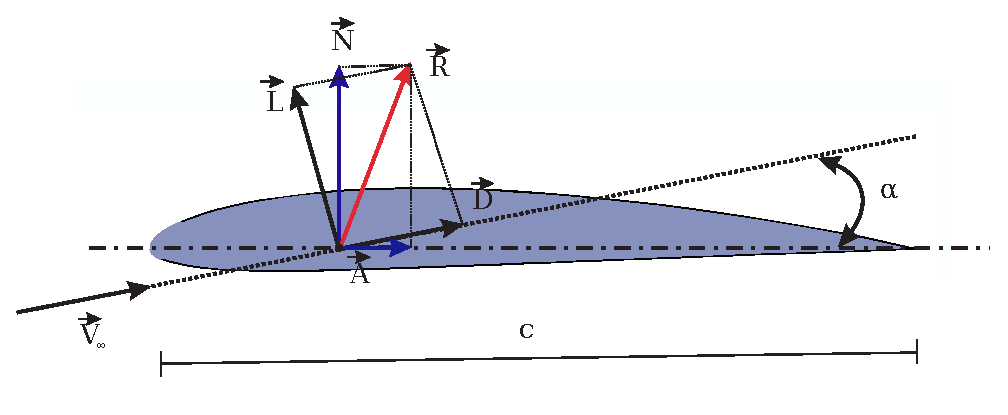
\includegraphics[scale=0.75]{imgmeca/Cuchilla.eps}  
		\caption{Fuerzas aereodin�micas que act�an en un perfil aereodin�mico.}
		\label{FuerzasCuchilla}
	\end{center}
\end{figure}

donde:\\
\null\qquad\qquad$\overrightarrow{v}_{\infty}$ representa la velocidad y la direcci�n del viento libre $[m/s]$.\\
\null\qquad\qquad$\overrightarrow{\text{L}}$, fuerza de sustentaci�n que act�a perpendicularmete a $\overrightarrow{v}_{\infty}$.\\
\null\qquad\qquad$\overrightarrow{\text{D}}$, fuerza de arrastre que act�a en direcci�n paralela a $\overrightarrow{v}_{\infty}$.\\
\null\qquad\qquad$\overrightarrow{\text{R}}$, fuerza resultante que act�a sobre el perfil aereodin�mico $[N]$.\\
\null\qquad\qquad$c$, l�nea de cuerda que conecta el borde superior e inferior del perfil.\\
\null\qquad\qquad$\overrightarrow{\text{N}}$, fuerza normal, perpendicular a la l�nea de cuerda $[N]$.\\
\null\qquad\qquad$\overrightarrow{\text{A}}$, fuerza axial, paralela a la l�nea de cuerda $[N]$.\\

Se pueden expresar mediante los siguiente modelos matem�ticos mostrados en \ref{eq:Rotor1} y \ref{eq:Rotor2} que representan las relaciones geom�tricas de las variables previamente mencionadas:

\begin{align}
 \label{eq:Rotor1}
\overrightarrow{\text{N}} = \overrightarrow{\text{L}}\text{cos}( \alpha) + \overrightarrow{\text{D}}\text{sen}( \alpha ) 
\end{align}

\begin{align}
 \label{eq:Rotor2}
\overrightarrow{\text{A}} = - \overrightarrow{\text{L}}\text{sen}( \alpha )  + \overrightarrow{\text{D}}\text{cos}( \alpha )
\end{align}

donde $\alpha$ representa el �ngulo de ataque del viento libre.\\

Por otro lado, se pueden denotar las fuerzas de sustentaci�n y de arrastre por medio de los coefcientes no dimensionales de sustentaci�n $C_l$ y de arrastre $C_d$, seg�n se muestra en las ecuaciones \ref{eq:Rotor3} y \ref{eq:Rotor4}.

\begin{align}
 \label{eq:Rotor3}
C_l = \frac{L}{\frac{1}{2} \rho v_{\infty}^{2} c}
\end{align}

\begin{align}
 \label{eq:Rotor4}
C_d = \frac{D}{\frac{1}{2} \rho v_{\infty}^{2} c}
\end{align}

El perfil aereodin�mico debe poseer un buen rendimiento a velocidades subs�nicas ($M < 1$) y una geometr�a adecuada para generar el mayor arrastre posible cuando el flujo del viento act�e de manera perpendicular a la superficie de la h�lice.\\

Las caracter�sticas propias del descenso del veh�culo cient�fico ayudan al momento de seleccionar el  perfil aereodin�mico. Primeramente, se debe tener en cuenta que, debido a las dimensiones del contenedor en donde ser� alojado el veh�culo cient�fico, no hay espacio para ubicar mecanismos de control activo del �ngulo de ataque de la h�lice. En segunda instancia, el perfil aereodin�mico tiene que poseeer la mayor curvatura posible en la l�nea de la cuerda de modo que esta geometr�a ayude a generar el mayor arrastre durante la ca�da (\cite{}, \cite{}, \cite{}). En la Tabla \ref{Perfiles} \footnote{Los valores mostrados corresponden a un �ngulo de ataque $\alpha = 1^{\text{o}}$} se presentan los perfiles aereodin�micos considerados para la selecci�n.

\begin{table}[H]
	\begin{center}
		\caption{Perfiles aereodin�micos considerados para velocidades subs�nicas.}
		\label{Perfiles}
		\resizebox{13cm}{!} {
			\begin{tabular}{m{4cm}m{3cm}m{3cm}m{4cm}}
				\multicolumn{4}{c}{}\tabularnewline
				\toprule
				\multicolumn{1}{c}{\textbf{Perfil aereodin�mico}} & \multicolumn{1}{c}{\textbf{Espesor m�ximo}} & \multicolumn{1}{c}{\textbf{Curvatura m�xima}} & \multicolumn{1}{c}{\textbf{$C_l$ m�ximo (Re = 50,000)}}\tabularnewline \hline \tabularnewline
				
				\multicolumn{1}{c}{NACA2412} & \multicolumn{1}{c}{12.0\% a 30.0 \% } &\multicolumn{1}{c}{2.0\% a 40.0\% }& \multicolumn{1}{c}{-0.1224} \tabularnewline
				\multicolumn{1}{c}{FX 63 - 137} & \multicolumn{1}{c}{13.7\% a 30.9 \% } &\multicolumn{1}{c}{6.00\% a 53.3\% }& \multicolumn{1}{c}{0.1919} \tabularnewline
				\multicolumn{1}{c}{MA 409} & \multicolumn{1}{c}{6.70\% a 23.8 \% } &\multicolumn{1}{c}{3.3\% a 49.3\% }& \multicolumn{1}{c}{0.0996} \tabularnewline
				\multicolumn{1}{c}{SG 6043} & \multicolumn{1}{c}{10.0\% a 32.1 \% } &\multicolumn{1}{c}{5.1\% a 53.3\% }& \multicolumn{1}{c}{-0.0091} \tabularnewline
				\multicolumn{1}{c}{E423} & \multicolumn{1}{c}{12.5\% a 23.7 \% } &\multicolumn{1}{c}{9.5\% a 41.4\% }& \multicolumn{1}{c}{-0.2184} \tabularnewline
				\bottomrule
			\end{tabular}
		}
	\end{center}
\end{table}

Ahora bien, como se puede observar en la Tabla \ref{Perfiles}, el perfil aereodin�mico que presenta las mejores caracter�sticas para la aplicaci�n es el perfil WORTMANN FX 63 - 137. No obstante, la informaci�n que se encuentra en la Tabla \ref{Perfiles} s�lo permite conocer el coeficiente de sustentaci�n $C_l$. Para poder obtener el coeficiente de arrastre $C_d$ del mismo perfil aereodi�nmico se recurre a la base de datos de la Universidad de Illinois \cite{}, la cual otorga un valor adimensional $C_d = 0.0470$.\\

La base de datos anteriormente mencionada tambi�n ofrece coordenadas del perfil aereodin�mico que pueden ser importadas en alg�n software de dise�o por compuadora para crear un modelo 3D del perfil aerodin�mico. En la figura \ref{fig:Plot} se muestra una previsualizaci�n del perfil aereodin�mico a utilizar.\\

\begin{figure}[H]
	\begin{center}
		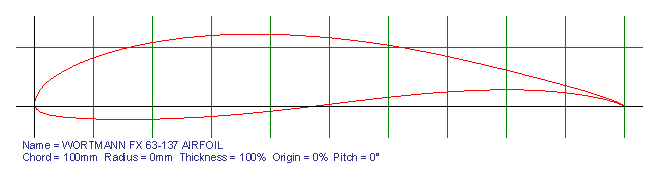
\includegraphics[scale=0.8]{imgmeca/Plot.eps}  
		\caption{Perfil aereodin�mico WORTMANN FX 63 -163. \label{fig:Plot}}
	\end{center}
\end{figure}


\begin{figure}[H]
	\begin{center}
		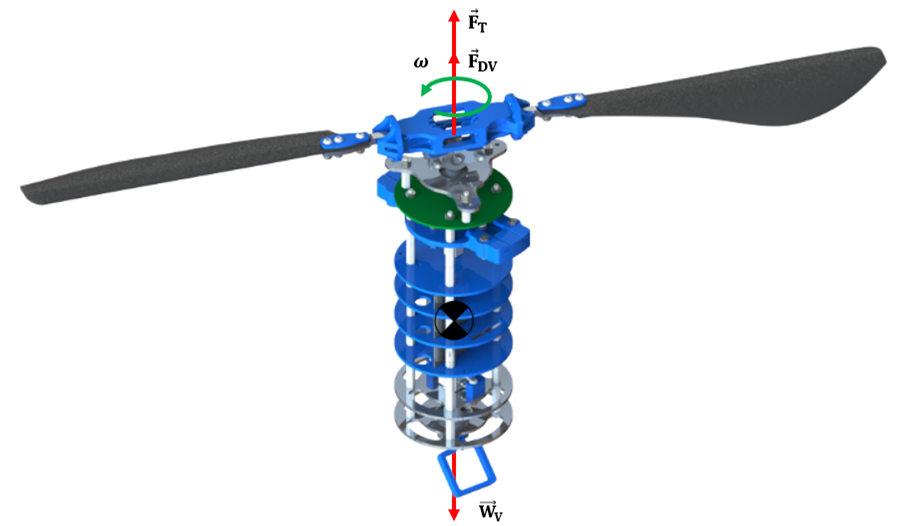
\includegraphics[scale=0.50]{imgmeca/Vehiculo.png}  
		\caption{Fuerzas que act�an en el veh�culo cient�fico durante el descenso por autorrotaci�n. \label{Vehiculo}}
	\end{center}
\end{figure}

Antes de continuar con el an�lisis del perfil aereodin�mico es importante recordar las caracter�sticas del descenso del veh�culo cient�fico una vez que es liberado del contenedor. En la figura \ref{Vehiculo} se pueden observar las fuerzas que act�an en el veh�culo cient�fico (considerando que el descenso es solamente vertical) donde:\\

\null\qquad$\overrightarrow{\text{F}}_{\text{DV}}$, fuerza de arrastre generada por la geometr�a del veh�culo cient�fico $[N]$.\\
\null\qquad$\overrightarrow{\text{F}}_{\text{T}}$, empuje generado por el movimiento de las h�lices $[N]$.\\
\null\qquad$\omega$, velocidad angular del rotor  $[rad/s]$.\\
\null\qquad$\overrightarrow{\text{W}}_{\text{v}}$, peso del veh�culo cient�fico $[N]$.\\

Una vez seleccionado el perfil aereodin�mico se deben de obtener las dimensiones del mismo. Para ello, en \cite{} se da un modelo matem�tico que relaciona la longitud de la cuerda del perfil aereodin�mico $c$, la magnitud de la velocidad generada por el movimiento del rotor $v_p$, la densidad $\rho$ y viscocidad $\mu$ del fluido, tal como se muestra en la ecuaci�n \ref{eq:Rotor10}.

\begin{eqnarray}
\label{eq:Rotor10}
\text{Re} = \frac{\rho v_p c}{ \mu }
\end{eqnarray}

Por lo regular, las bases de datos de perfiles aereodin�micos otorgan valores del coeficiente de sustentaci�n y arrastre para n�meros de Reynolds mayores a 50 000, de modo que los c�lculos realizados se har�n con ese valor. Es preferible que el flujo se encuentre lo m�s cercano a un flujo laminar. Se resuelve la ecuaci�n \ref{eq:Rotor10} considerando que $\text{Re} = 50\text{x}10^{3}$ , $\rho = 1.225 [kg/m^3]$,
$ \mu = 1{.}8 \text{x} 10^{-5} [\text{N} \cdot \text{s} \cdot \text{m}^{\text{-2}}]$, y que la velociad $\overrightarrow{v}_{\text{p}} [\text{m} \cdot \text{s}^{\text{-1}}]$ debida al giro del rotor es la misma que la velocidad de descenso  del veh�culo cient�fico, la cual oscilar� entre los $10 [m/s]$ y $15 [m/s]$. Los valores de $c$ para diferentes velocidades se muestran en la Tabla \ref{valoresc}.

\begin{table}[H]
	\begin{center}
		\caption{Longitud de la cuerda a diferentes valores de velocidad de descenso.}
		\label{valoresc}
		\resizebox{3cm}{!} {
			\begin{tabular}{m{2cm}p{3cm}}
				\multicolumn{2}{c}{}\tabularnewline
				\toprule
				\multicolumn{1}{c}{\textbf{$\overrightarrow{v}_{\text{p}}$ [m/s]}} & \multicolumn{1}{c}{\textbf{$c [m]$}}\tabularnewline \hline \tabularnewline
				
				\multicolumn{1}{c}{10} & \multicolumn{1}{c}{0.0735}\tabularnewline
				\multicolumn{1}{c}{11} & \multicolumn{1}{c}{0.0668}\tabularnewline
				\multicolumn{1}{c}{12} & \multicolumn{1}{c}{0.0612}\tabularnewline
				\multicolumn{1}{c}{13} & \multicolumn{1}{c}{0.0565}\tabularnewline
				\multicolumn{1}{c}{14} & \multicolumn{1}{c}{0.0525}\tabularnewline
				\multicolumn{1}{c}{15} & \multicolumn{1}{c}{0.0490}\tabularnewline
				\bottomrule
			\end{tabular}
		}
	\end{center}
\end{table}

En vista de que uno de los factores m�s cr�ticos a considerar para el desarrollo del CanSat es la masa del mismo, se eligi� la longitud de la cuerda que corresponde a una velocidad de descenso de $13 [m/s]$.\\

Una vez que se han determinado los valores del coeficente de arrastre y sustentaci�n, as� como las dimensiones  de la cuerda del perfil aereodin�mico, es posible demostrar que el movimiento de las h�lices generar� una fuerza de empuje $\overrightarrow{\text{F}}_{\text{T}}$ que, junto con la fuerza de arrastre producida por la geometr�a de las h�lices, ser�n capaces de mantener una velocidad de descenso constante.\\

Existen dos teor�as que relacionan las variables previamente mencionadas con el empuje que se genera: la Teor�a del Elemento de la Cuchilla presentada por W. Froude \cite{Froude} y que es un modelo no tan complejo que permite predecir el comportamiento de un cierto tipo de geometr�a; por otro lado est� la Teor�a del Impulso, la cual fue desarrollada por Rankine \cite{Rankine} y se basa en la idea de que cualquier h�lice produce empuje.\\

La Teor�a del Elemento de la Cuchilla es las m�s apropiada para el desarrollo de los c�lculos debido a que esta teor�a considera el n�mero de h�lices, las caracter�sticas del perfil aereodin�mico, la forma de la h�lice, la distribuci�n de la torsi�n de la h�lice y los efectos de compresibilidad. Como se puede observar en la figura \ref{BET}, la distancia desde el eje de la h�lice a la l�nea central de cada elemento esta denotada por $\text{R'}$, y $\text{dR}$ es el ancho del elemento. $\text{R}$ es la distancia desde el eje de la h�lice hasta la punta de la pala, tambi�n llamado radio de punta. Esta representaci�n gr�fica es v�lida para otras geom�tr�as relacionadas con un perfil aereodin�mico.

\begin{figure}[H]
	\begin{center}
		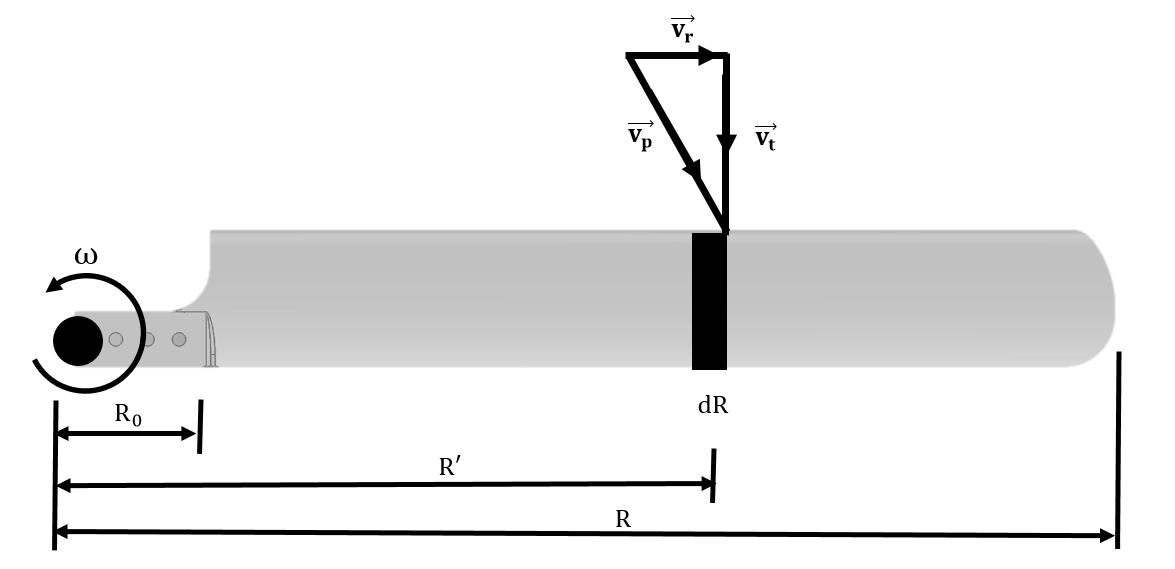
\includegraphics[scale=0.22]{imgmeca/BET.png}  
		\caption{Aplicaci�n de la teor�a del elemento de la cuchilla en una h�lice. }
		\label{BET}
	\end{center}
\end{figure}

Para hacer m�s comprensible la representaci�n de esta teor�a se usar� la adaptaci�n de los libros de texto de Glauert \cite{Glauert} y Weick \cite{Weick}.\\

En la figura \ref{BETFuerzas} se pueden apreciar las diferentes fuerzas a las que es sometido el perfil aereodin�mico, de acuerdo con el m�todo de la teor�a del elemento de la cuchilla, donde $\theta$ est� compuesto por el �ngulo de ataque del perfil aereodin�mico $\alpha_{b}$ y el �ngulo de giro de la cuchilla con respecto al plano de la h�lice $\varphi$. El flujo al que est� expuesto el perfil aereodin�mico est� representado por $\overrightarrow{v}_{\text{p}}$. 

\begin{figure}[H]
	\begin{center}
		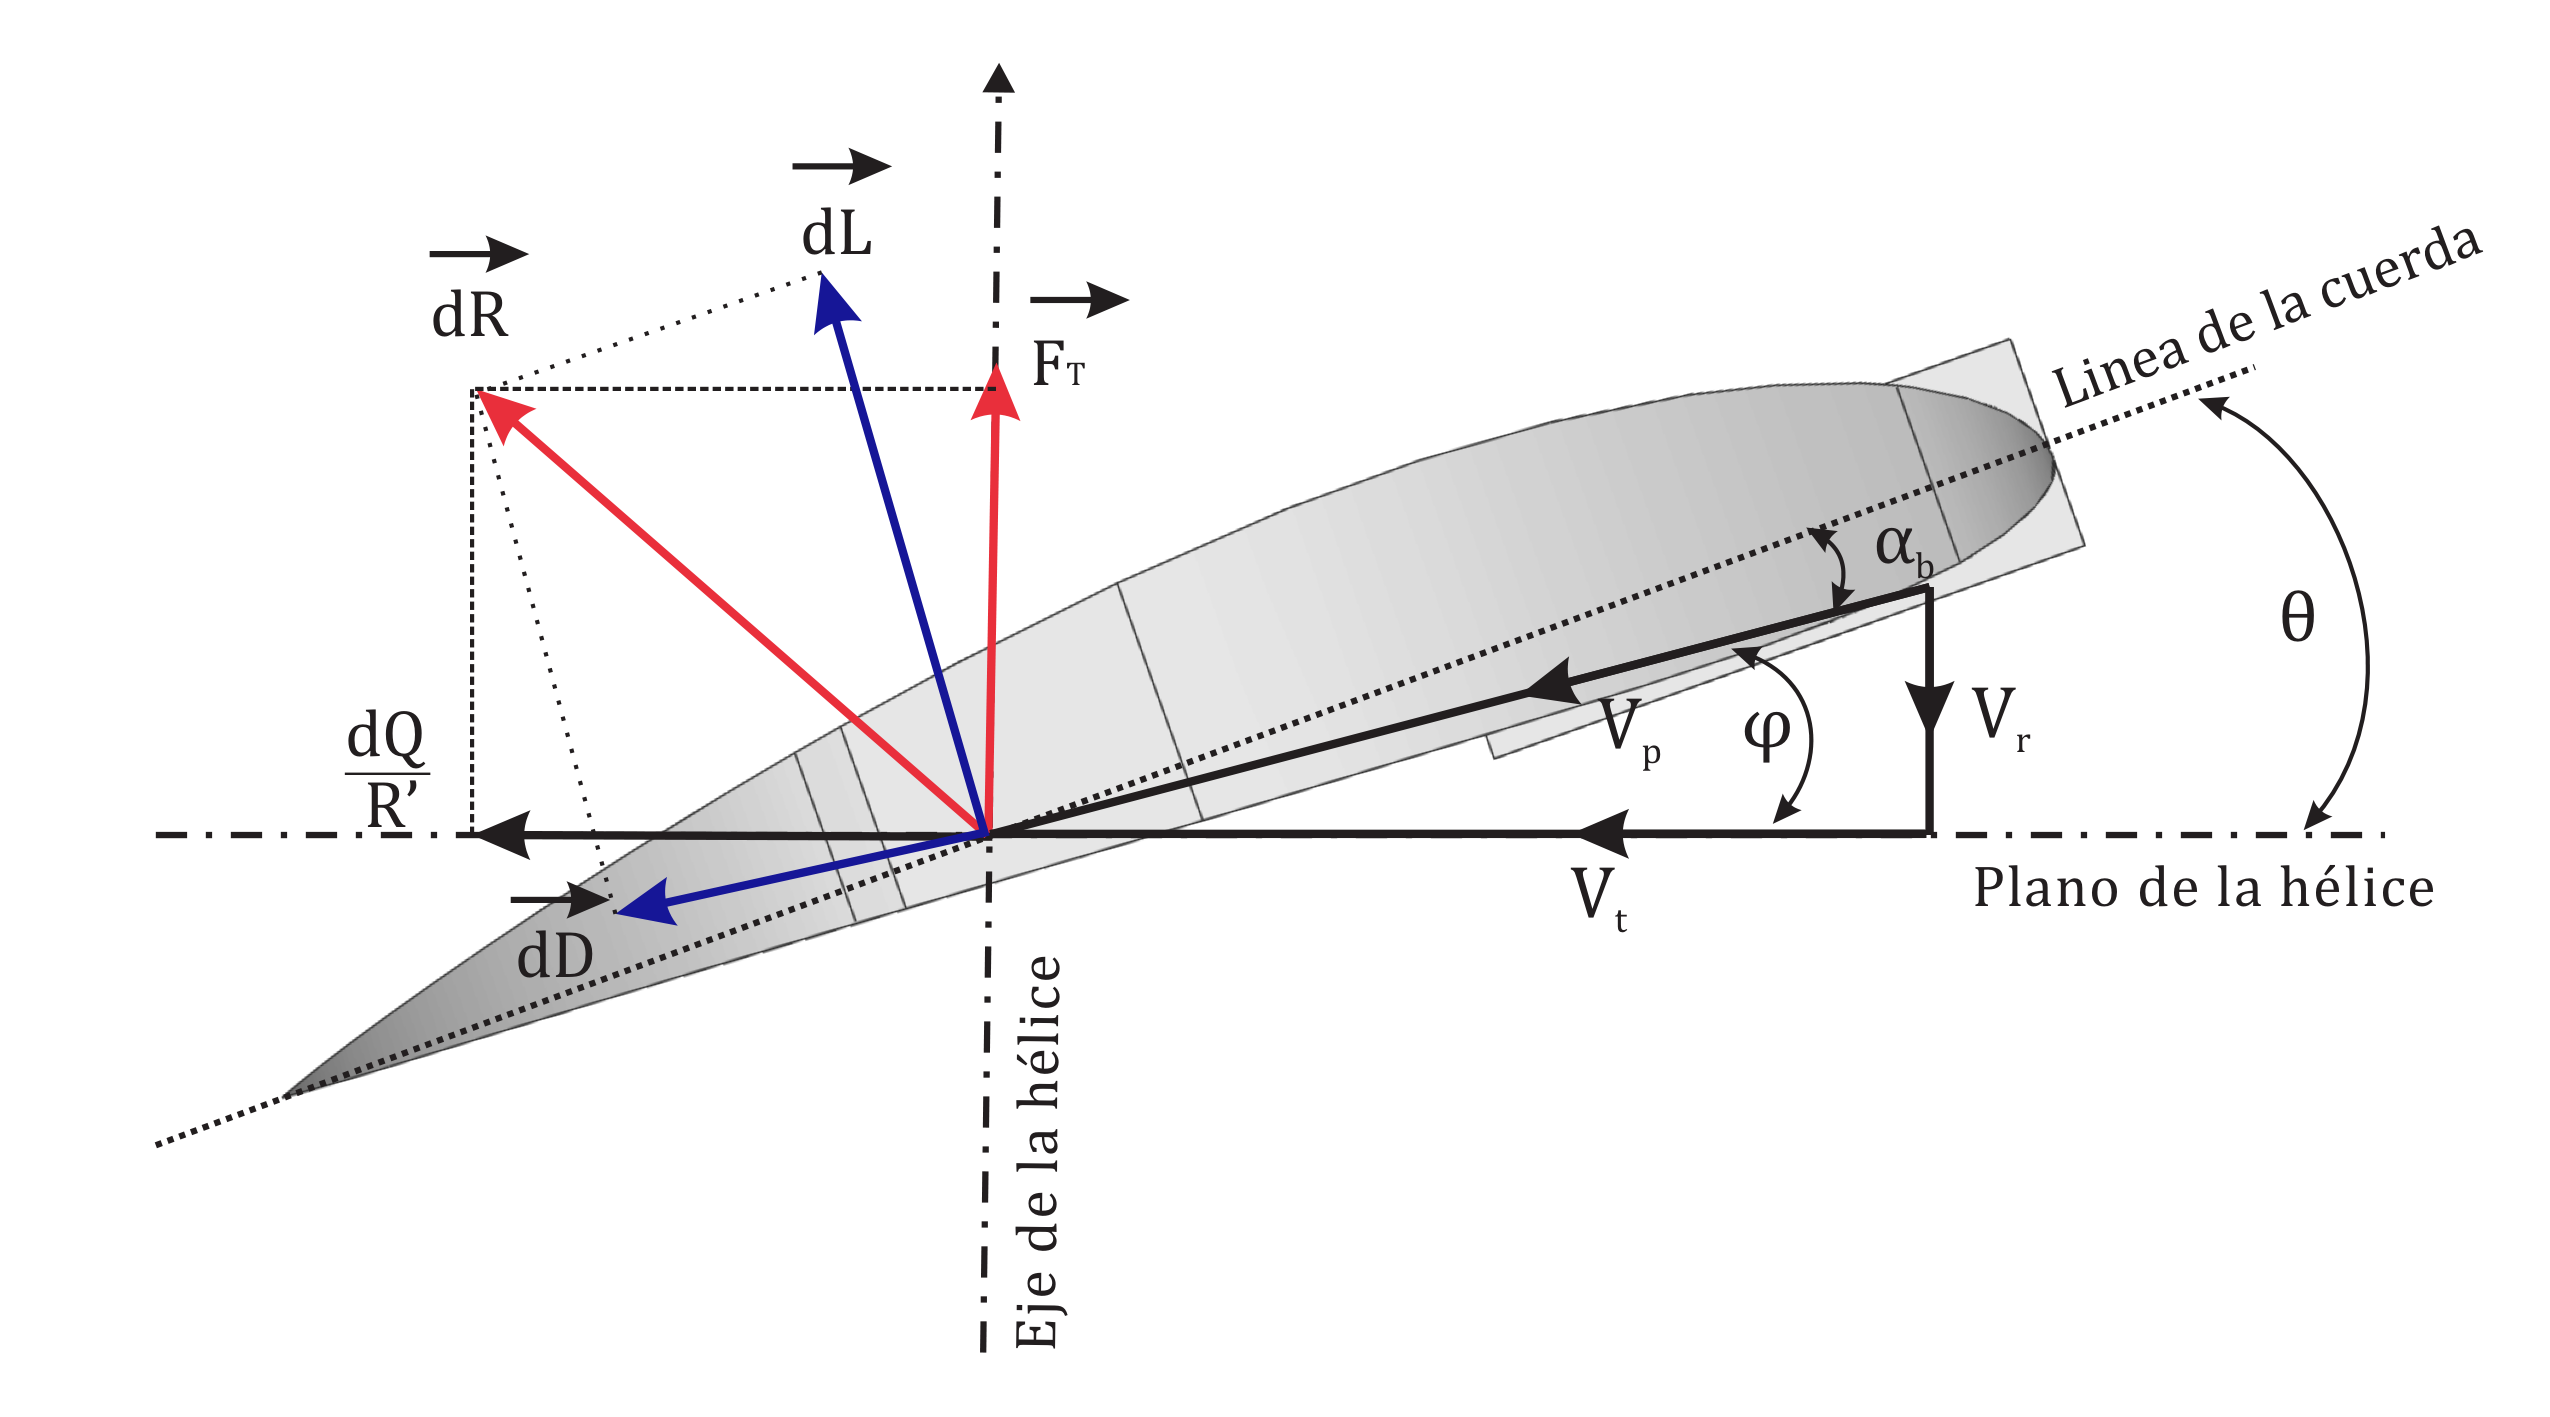
\includegraphics[scale=0.085]{imgmeca/BET5.png}  
		\caption{Definici�n de fuerzas y velocidades actuando en un elemento de la cuchilla.}
		\label{BETFuerzas}
	\end{center}
\end{figure}

Finalmente, despu�s de algunas simplificaciones, se obtienen las expresiones para la sustentaci�n $\overrightarrow{\text{dL}}$ y arrastre $\overrightarrow{\text{dD}}$ del perfil aereodin�mico seg�n las ecuaciones \ref{eq:sust} y \ref{eq:arra}, respectivamente.

\begin{align}
\label{eq:sust}
\overrightarrow{\text{dL}} = \frac{1}{2} \rho v_{vc}^{2} C_l (\alpha_{b}) c \text{N}_{\text{b}} \text{dR}
\end{align}

\begin{align}
\label{eq:arra}
\overrightarrow{\text{dD}} = \frac{1}{2} \rho v_{vc}^{2} C_d (\alpha_{b}) c \text{N}_{\text{b}} \text{dR}
\end{align}

donde:\\
\null\qquad\qquad$\text{N}_{\text{b}}$, n�mero de h�lices $[adimensional]$.\\
\null\qquad\qquad$\alpha_{b}$, �ngulo de ataque de la h�lice $[rad]$.\\

El empuje $\overrightarrow{\text{F}}_{\text{T}}$ y el torque $\text{dQ}$ pueden ser obtenidos de las siguientre transformaciones geom�tricas de \eqref{eq:sust} y \eqref{eq:arra}.

\begin{equation}
\label{eq:hipotesissustentacion}
\overrightarrow{\text{F}}_{\text{T}} =\overrightarrow{\text{dL}}\text{cos}(\varphi) - \overrightarrow{\text{dD}}\text{sen}(\varphi)
\end{equation}

\begin{equation}
\label{eq:hipotesistangencial}
\frac{\text{dQ}}{\text{R'}} = \overrightarrow{\text{dL}}\text{sen}(\varphi) + \overrightarrow{\text{dD}}\text{cos}(\varphi)
\end{equation}

Para poder utilizar la teor�a del elemento de la cuchilla en la autorrotaci�n se tomaron en cuenta los siguientes puntos \cite{}:

\begin{itemize}
	\item Se considera un comportamiento bidimensional en cada elemento de la cuchilla.
	\item La velocidad inducida, que es perpendicular al plano del rotor, se considera como una modificaci�n del �ngulo de ataque del rotor.
	\item La componente radial de la velocidad del viento es despeciable.
	\item cos ($\varphi$)  = 1, sen($\varphi$) = $\varphi$.
	\item $\overrightarrow{\text{dL}} >> \overrightarrow{\text{dD}}$  
\end{itemize}

Tomando en cuenta estas consideraciones, las ecuaciones \ref{eq:hipotesissustentacion} y \ref{eq:hipotesistangencial} quedan de la siguiente manera:

\begin{align}
\label{eq:sustentacion}
\overrightarrow{\text{F}}_{\text{T}} \approx \overrightarrow{\text{dL}} - \overrightarrow{\text{dD}} \cdot \varphi \approx \overrightarrow{\text{dL}}
\end{align}

\begin{align}
\frac{\text{dQ}}{\text{R'}} \approx \overrightarrow{\text{dL}}\cdot \varphi  + \overrightarrow{\text{dD}}
\end{align}

En vista de que el empuje $\overrightarrow{\text{F}}_{\text{T}}$ depende s�lo de la fuerza de sustentaci�n $\overrightarrow{\text{dL}}$, se puede aplicar el modelo de disco discreto el cual menciona que, debido a que durante el descenso por autorrotaci�n el rotor se encuentra en el r�gimen de estela turbulenta \footnote{Para velocidades de descenso medias, la estela se vuelve m�s turbulenta y el flujo es similar al de un cuerpo no aereodin�mico.}, se suele realizar la analog�a de considerar el rotor como un disco resistente impermeable.\\

El coeficiente de arrastre del disco impermeable $C_d$ suele tomar valores que van de 1.25 a 1.30, siendo 1.28 un valor muy empleado en las estimaciones de autorrotaci�n \cite{}.\\

Utilizando la segunda ley de Newton del movimiento se puede obtener una expresi�n para la estimaci�n de la velocidad del veh�culo cient�fico durante la etapa de descenso por autorrotaci�n de modo que la ecuaci�n 3.15 relaciona la velocidad del viento generada por el movimiento del veh�culo cient�fico $\overrightarrow{v}_{\text{vc}}$, donde $m_vc$ representa la masa del veh�culo cient�fico.\\

\begin{align}
\label{eq:EcuAuto}
- \overrightarrow{\text{F}}_{\text{T}} -  \overrightarrow{\text{F}}_{\text{DV}}   + \overrightarrow{\text{W}}_{\text{v}}  = m_vc \frac{d\overrightarrow{v}_{\text{vc}}}{dt}
\end{align} 

Desarrollando \ref{eq:EcuAuto} se obtine la siguiente expresi�n:

\begin{align}
\label{eq:simplificadovehiculo}
-\frac{\rho S_d C_Dd v_vc^{2}}{2} - \frac{\rho S_v C_Dv v_vc^{2}}{2} + m_vc g =  m_vc \frac{dv_vc}{dt}
\end{align}

donde:\\

\null\qquad$S_v$, superficie efectiva del veh�culo cient�fico $[m^2]$.\\
\null\qquad$C_D$, coeficiente de arrastre de la geometr�a del veh�culo cient�fico $[adimensional]$.\\
\null\qquad$S_d$, superficie del disco impermeable $[m^2]$.\\

Los resultados de resolver la ecuaci�n \ref{eq:simplificadovehiculo} se muestran en la figura \ref{fig:Grafica2}, donde se observa que la velocidad de descenso tiene un valor constante de $12.3437 [m/s]$ despu�s de que transcurren $2.0469[s]$.\\

\begin{figure}[H]
	\begin{center}
		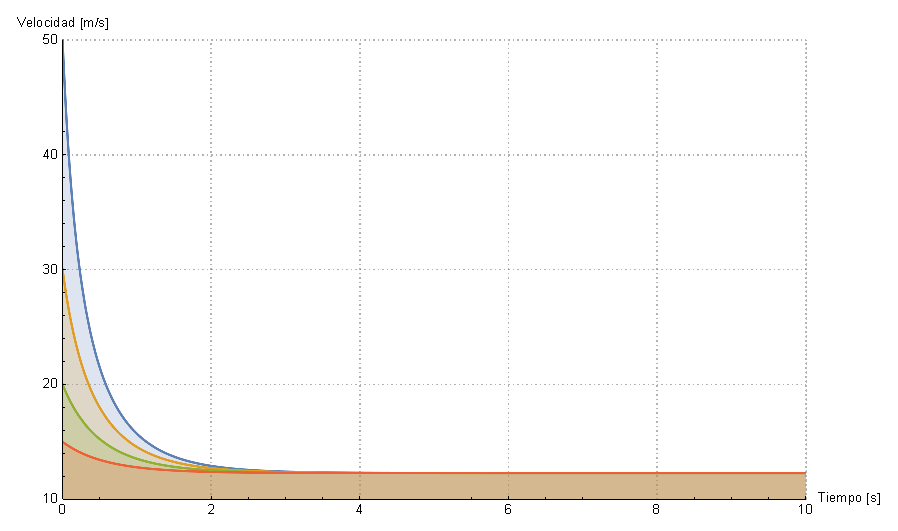
\includegraphics[scale=0.90]{imgmeca/Grafica2.eps}  
		\caption{Estimaci�n de la velocidad de descenso del veh�culo cient�fico durante la etapa de autorrotaci�n. \label{fig:Grafica2}}
	\end{center}
\end{figure}

Una vez que se obtuvieron las dimensiones de las h�lices se dise�� el mecanismo de rotor del SRV-A. Los componenete mec�nicos que conforman este mecanismo se muestran en las figura \ref{img:Partesrotor}. Como elementos de sujeci�n se utilizaron tornillos M3 y M2 de diferentes longitudes con su respectiva tuerca de bloqueo con inserto de nylon.\\

Durante la etapa de dise�o uno de los cambios m�s significativos fue la geometr�a del monoblock. Este elemento en un principio era un componente que estaba conformado por varias piezas, como se observa en la figura \ref{img:Monoblock}. Uno de los motivos que orillaron a realizar el monoblock en una sola pieza fue reducir la masa y la cantidad de componentes. Con la reducci�n de componentes se evitan problemas con la vibraci�n durante el ascenso y descenso del veh�culo cientif�co.\\

\begin{figure}[H]
	\begin{center}
		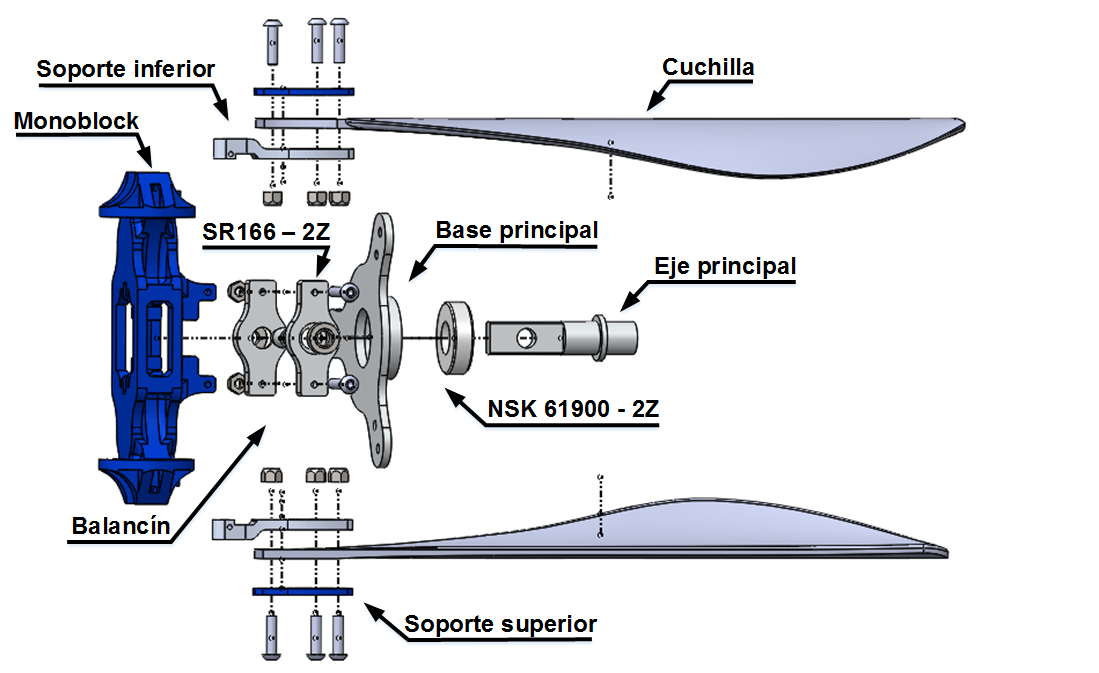
\includegraphics[scale=0.47]{imgmeca/Partesrotor.png}  
		\caption{Componenetes del SRV-A. \label{img:Partesrotor}}
	\end{center}
\end{figure}
 

\begin{figure}[H]
	\begin{center}
		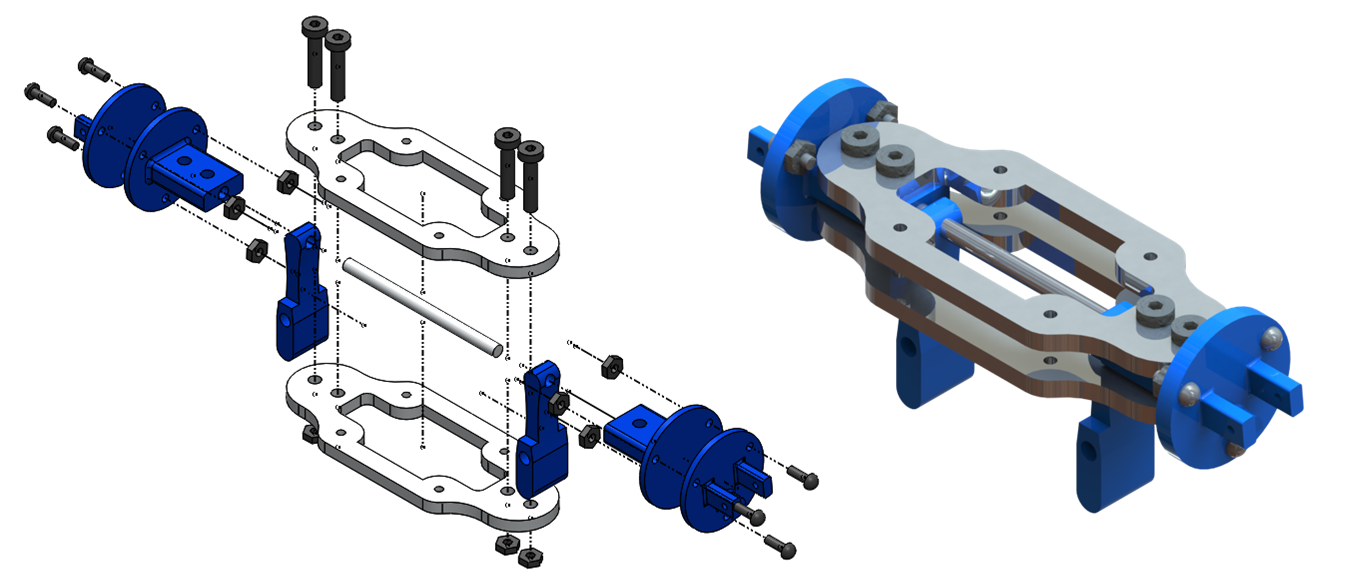
\includegraphics[scale=0.32]{imgmeca/Monoblock.png}  
		\caption{Dise�o original del monoblock. \label{img:Monoblock}}
	\end{center}
\end{figure}


El rotor contiene un elemento que le permite balancear los cambios de orientaci�n de la velocidad del viento, con la finalidad de mantener un descenso vertical. En la figura \ref{img:balanceo} se muestran los dos casos en los que el balanc�n trabaja. Este mecanismo tambi�n permite controlar de manera pasiva la orientaci�n de la c�mara del SRD.

\begin{figure}[H]
	\begin{center}
		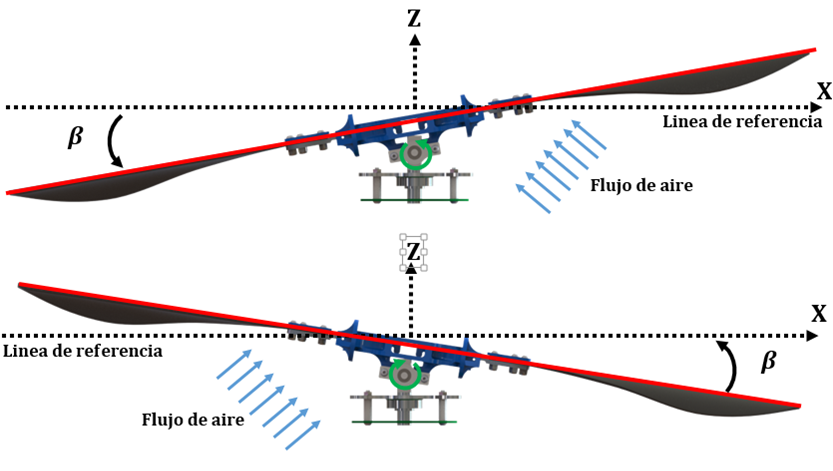
\includegraphics[scale=0.55]{imgmeca/Balanceo.png}  
		\caption{Funcionamiento del sistema de balanceo. \label{img:balanceo}}
	\end{center}
\end{figure}

}

\newpage
		\subsection{Sistema de Liberaci�n del Vehiculo Cient�fico} \label{sistSLVC}
% !TeX encoding = ISO-8859-1

{\parindent0pt

El Sistema de Liberaci�n del Veh�culo Cient�fico tiene como funci�n mantener unidos al veh�culo cient�fico y al contenedor durante la etapa de ascenso hasta el apogeo y durante la primera etapa de descenso hasta los 100 [m]. El SLVC realiza la funci�n $f_{4{.}5}-$\textit{Liberar veh�culo cient�fico}. A los $100[m]$ el SLVC ser� activado por el STD y el veh�culo cient�fico se separar� del contenedor. La figura \ref{img:partesliberacion} muestra al mecanismo del SLVC. Como elementos de sujeci�n se utilizaron tornllos M3 y M2 con su respectiva tuerca de bloqueo con inserto de nylon.

\begin{figure}[H]
	\begin{center}
		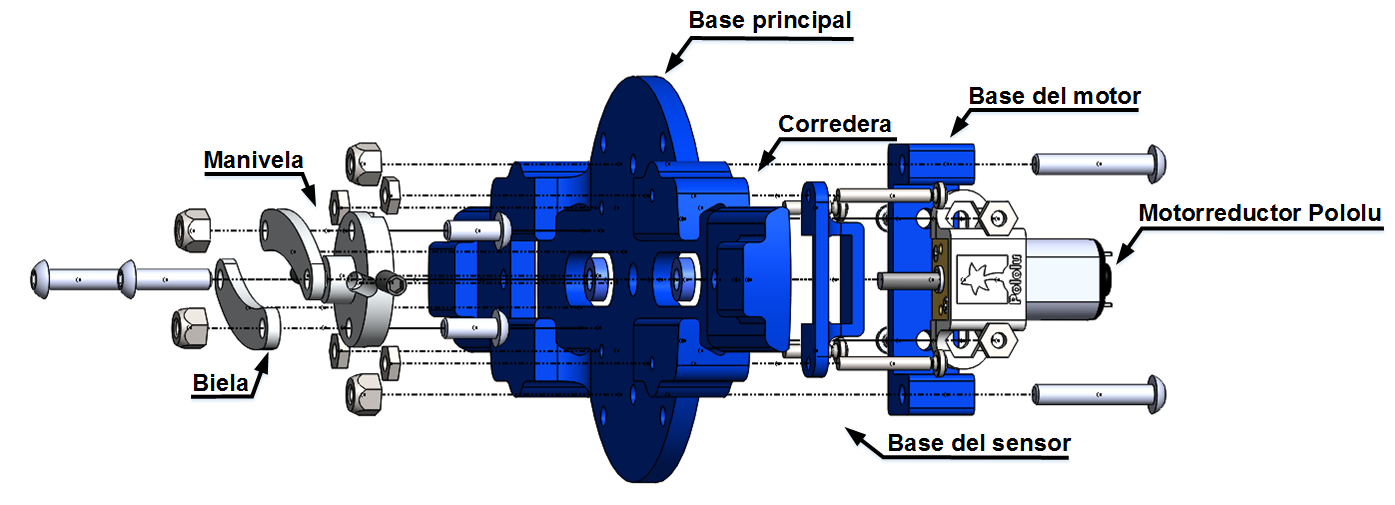
\includegraphics[scale=0.35]{imgmeca/Partesliberacion.png}  
		\caption{Elementos que conforman el sistema de liberaci�n del veh�culo cient�fico.}
		\label{img:partesliberacion}
	\end{center}
\end{figure}


El SLVC es un mecanismo de biela-manivela-corredera doble. El motor de CD est� acoplado mec�nicamente a la biela: cuando el motor gira, la manivela mueve a la corredera. Las correderas est�n atoradas con la estructura del contenedor, por lo tanto, el veh�culo cient�fico se libera cuando las correderas se contraen. En la figura \ref{img:partesliberacion} se pueden ver los interruptores de extremos de carrera (puestos en las bases de sensor). El mecanismo tiene un interruptor de inicio de carrera en un lado y un interruptor de final de carrera en el otro. La figura \ref{img:slvcsecuencia} muestra la secuencia de activaci�n del mecanismo.

\begin{figure}[H]
	\begin{center}
		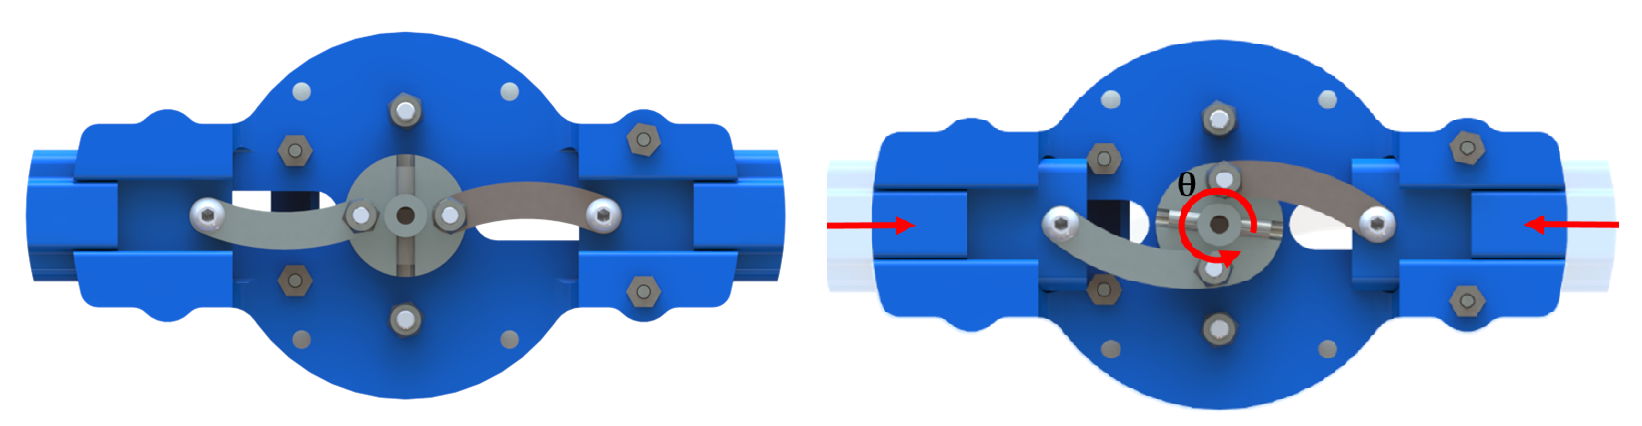
\includegraphics[scale=0.30]{imgmeca/SLVCsecuencia.png}  
		\caption{Secuencia de activaci�n del mecanismo del SLVC.}
		\label{img:slvcsecuencia}
	\end{center}
\end{figure}

Los interruptores de extremos de carrera son utilizados como se�ales de retroalimentaci�n del movimiento del mecanismo. Dependiendo de qu� interruptor est� activado el microcontrolador puede determinar el estado del mecanismo: correderas extendidas (interruptor de final de carrera presionado) o correderas contra�das (interruptor de inicio de carrera presionado). Estas se�ales permiten activar el motor de CD por �nicamente el tiempo necesario, ahorrando energ�a de las bater�as.\\

\subsubsection*{Selecci�n de materiales}
Las manivelas y la biela son uno de los puntos m�s cr�ticos del mecanismo presentado en la figura \ref{img:partesliberacion} ya que son los que estar�n sometidos a flexi�n durante el despegue del CanSat. Por esta raz�n, la aleaci�n de aluminio AA 6061 fue seleccionada para su fabricaci�n, adem�s de ser una de las aleaciones m�s comunes. Las manivelas y la biela son piezas muy peque�as por lo que no representan un valor de masa muy elevado.\\

Para el caso de la base y las correderas se necesita poca fricci�n entre ambos componentes para un desacople r�pido. Fabricar de aluminio estas piezas representar�a mucha masa para el CanSat por lo que se propone el uso del la impresi�n con ABS junto con un tratamiento con vapor de acetona para eliminar la mayor cantidad de imperfecciones producidas por el proceso de deposici�n de material y as� reducir la fricci�n entre componentes.\\

}
		
\newpage
		\subsection{Sistema de Registro de Descenso} \label{sistSRD}
% !TeX encoding = ISO-8859-1

{\parindent0pt

EL Sistema de Registro de Descenso est� encargado de orientar la c�mara y grabar video durante el descenso del CanSat; el SRD cumple con la funci�n $f_{4{.}1}-$\textit{Registrar descenso}. Para realizar dicha funci�n, el sistema cuenta con un mecanismo de compensaci�n en azimut para mantener la c�mara orientada, y tambi�n cuenta con la c�mara para realizar la grabaci�n del video. El mecanismo del SRD se muestra en la figura \ref{fig:MecAzimut}.

\begin{figure}[H]
	\begin{center}
		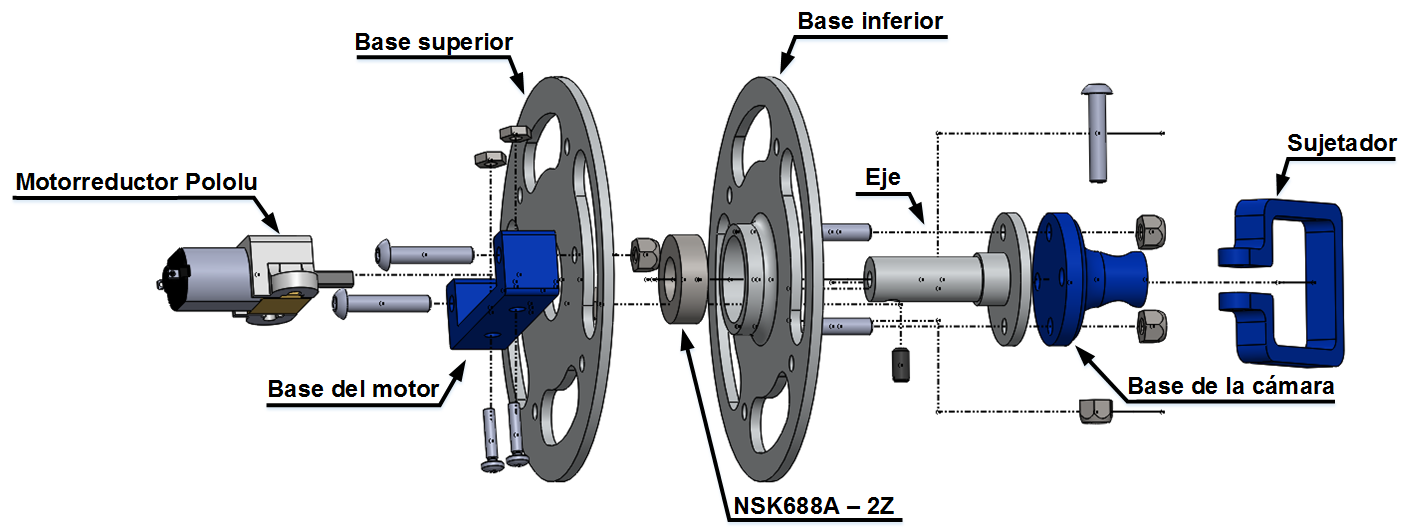
\includegraphics[scale=0.35]{imgmeca/Partesregistro.png}  
		\caption{\label{fig:MecAzimut}Elementos que conforman el mecanismo de orientaci�n de la c�mara del SRD.}
	\end{center}
\end{figure}


Este sistema debe mantener orientada la c�mara de acuerdo con la posici�n inicial al momento de iniciar la misi�n. El dise�o de este sistema se desarroll� bajo la suposici�n de que el sistema de rotor, gracias a su mecanismo de balanc�n, ayudar� a mantener el CanSat en una posici�n vertical durante el descenso. Bajo esta suposici�n se propuso el control por regulaci�n de un s�lo grado de libertad (azimut). El control del �ngulo de azimut se realiza por medio de un motor de CD con sistema de engranes para reducci�n y una base m�vil rotatoria acoplada al eje del motor. Este mecanismo es el mostrado en la figura \ref{fig:MecAzimut}. El motor usado es un motorreductor 380:1 con velocidad nominal de 85 $[rpm]$. El motor cuenta con un enconder de cuadratura que proporciona 12 pulsos por revoluci�n del eje del motor (sin la etapa de reducci�n por engranes).\\

Aunque el sistema cuenta con una velocidad de c�mputo elevada, se propone un controlador de dos tareas. La primera tarea es realizar el c�lculo del error en intervalos de $0.5\text{[s]}$, mientras que la segunda tarea es compensar el error en intervalos de $0.01\text{[s]}$. Esto evita que el sistema se sature con tareas impuestas en intervalos cortos de tiempo y permite mantener tiempos fijos para implementar el controlador. El control del motor est� basado en un control por PWM para la regulaci�n de la velocidad y un puente H para el control de la direcci�n de giro del motor.\\

Este sistema fue simulado en el ambiente de Simulink considerando para ello un incremento de velocidad del motor lineal con respecto al incremento en el ciclo de trabajo. El sistema simulado puede observarse en la figura \ref{img:Sis_Control}

\begin{figure}[H]
	\centering
	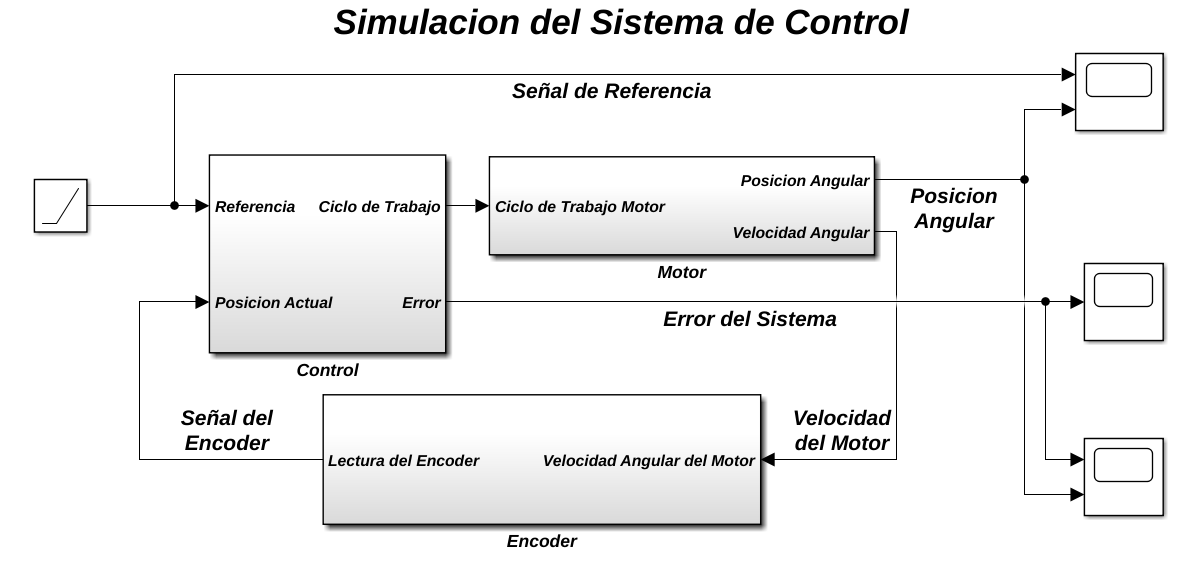
\includegraphics[scale=0.3]{imgmeca/SRD/Esquema.png}
	\caption{Simulaci�n del control de orientaci�n de la c�mara.}
	\label{img:Sis_Control}
\end{figure}


De este sistema se realizaron dos simulaciones: la primera simulaci�n tiene como referencia un escal�n con amplitud equivalente a $100$[$^\circ$], mientras que la segunda simulaci�n tiene como entrada una se�al rampa con una pendiente equivalente a $100$[$^\circ/s$].\\

El control es del tipo PID y cuenta con valores de $50$, $0.01$ y $0.01$, en sus ganancias proporcional, integral y derivativa, respectivamente. Estas ganancias fueron obtenidas de manera emp�rica.\\

En el primer caso se obtuvo la se�al mostrada en la figura \ref{img:Sim1_Img1}

\begin{figure}[H]
	\centering
	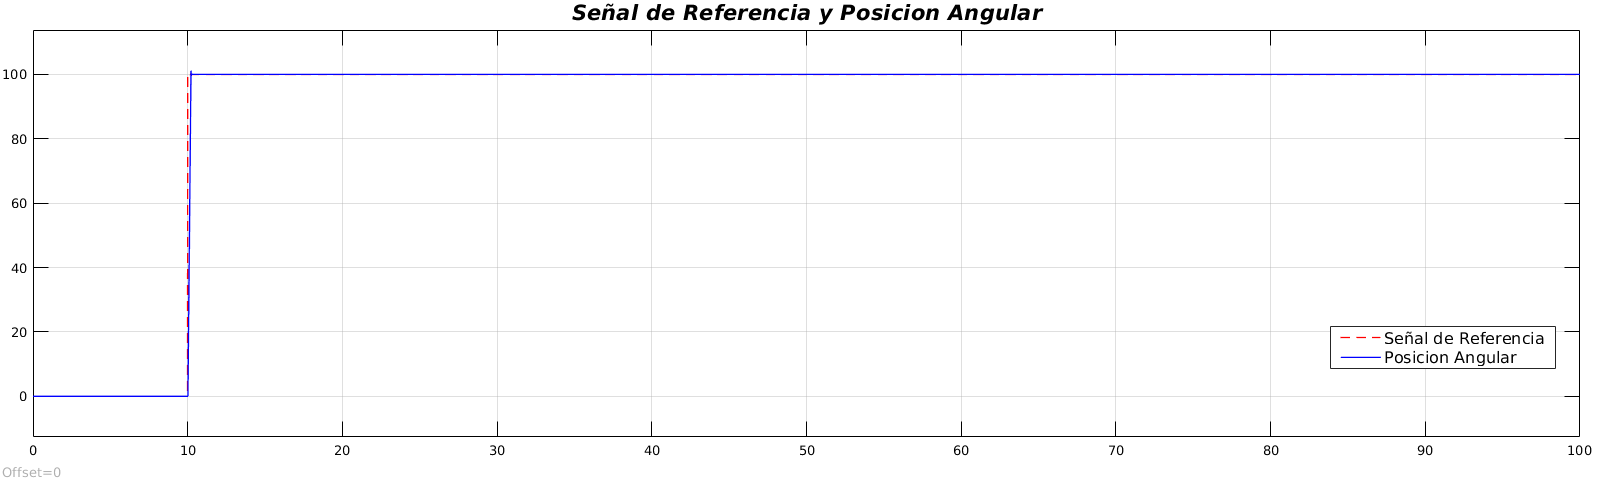
\includegraphics[scale=0.3]{imgmeca/SRD/Sim1_Img1.png}
	\caption{Primera Simulaci�n. Entrada Escal�n. Sin aumento. Referencia y Posici�n Angular.}
	\label{img:Sim1_Img1}
\end{figure}

En la figura \ref{img:Sim1_Img1} se aprecia la respuesta completa dentro de un tiempo de simulaci�n de $100$[s], sin embargo, en la figura \ref{img:Sim1_Img2} se hace un acercamiento al intervalo comprendido entre los $9.9$[s] y $10.4$[s].

\begin{figure}[H]
	\centering
	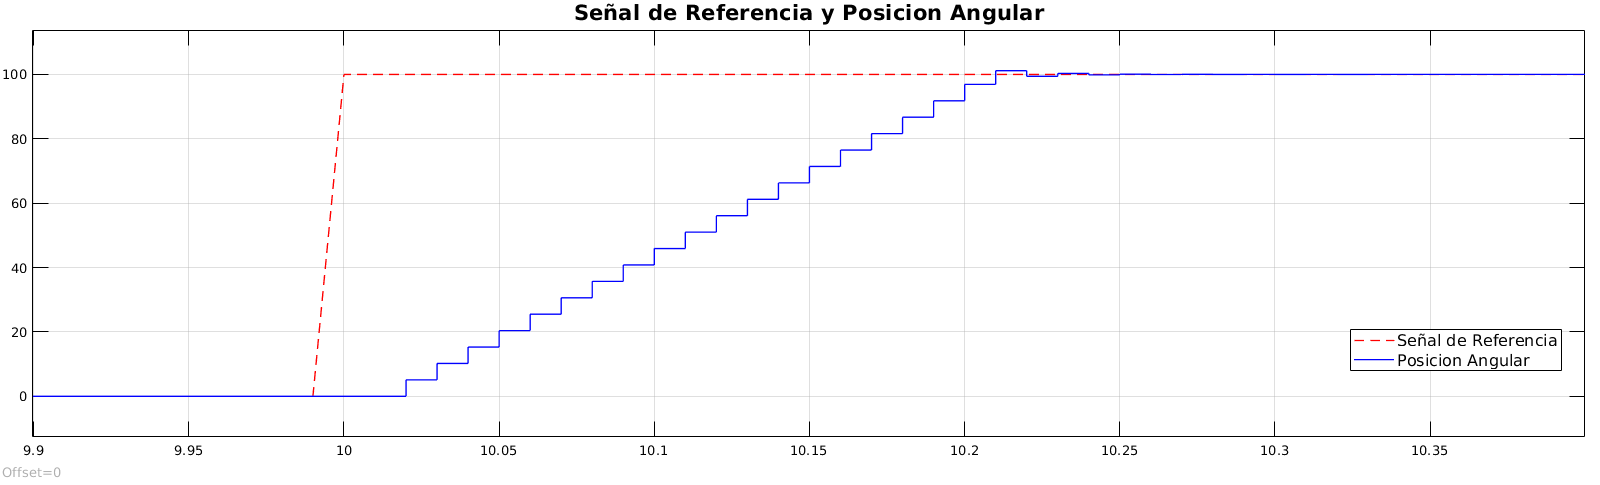
\includegraphics[scale=0.3]{imgmeca/SRD/Sim1_Img2.png}
	\caption{Primera Simulaci�n. Entrada Escal�n. Con aumento. Referencia y Posici�n Angular.}
	\label{img:Sim1_Img2}
\end{figure}

En la figura \ref{img:Sim1_Img2} se observa un sobreimpulso de $1.15$[$^\circ/s$] y un tiempo de establecimiento de aproximadamente $0.25$[s] para la referencia de $100$[$^\circ$].\\

En la figura \ref{img:Sim1_Img3}, que se encuentra dentro del mismo intervalo de tiempo que la figura \ref{img:Sim1_Img2}, se observa la din�mica del error a trav�s del tiempo y, aunque este adquiera valores mayores a las $100$ unidades dentro de los c�lculos, f�sicamente le es imposible llegar a ese valor debido a que el PWM se encuentra acotado de 0 a 100 unidades.

\begin{figure}[H]
	\centering
	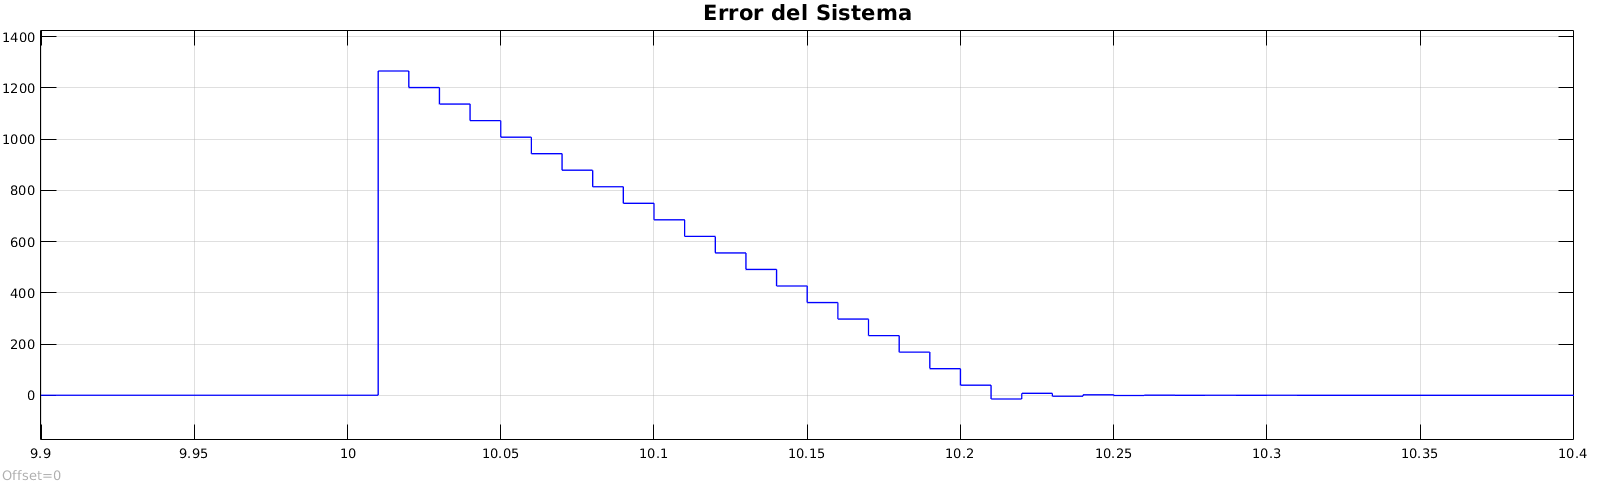
\includegraphics[scale=0.3]{imgmeca/SRD/Sim1_Img3.png}
	\caption{Primera Simulaci�n. Entrada Escal�n. Con aumento. Error del Sistema.}
	\label{img:Sim1_Img3}
\end{figure}

Para el segundo caso se muestra la respuesta en la figura \ref{img:Sim2_Img1}. El igual que en el caso anterior, se puede apreciar que el sistema sigue la referencia aunque no se aprecia con detalle como el sistema se va acercando a dicha referencia. Para un mayor detalle se muestra la figura \ref{img:Sim2_Img2} que presenta un acercamiento al intervalo comprendido entre los $0$[s] y $2$[s], y los $0$[$^\circ$] y $200$[$^\circ$].

\begin{figure}[H]
	\centering
	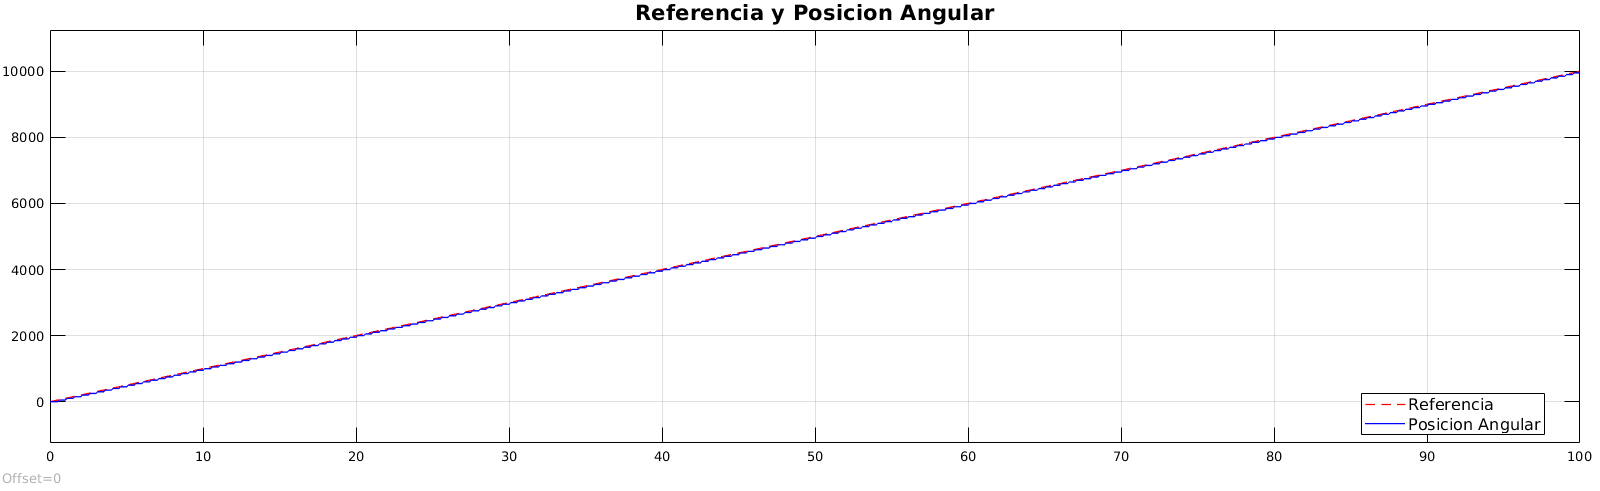
\includegraphics[scale=0.3]{imgmeca/SRD/Sim2_Img1.png}
	\caption{Segunda Simulaci�n. Entrada Rampa. Sin aumento. Referencia y Posici�n Angular.}
	\label{img:Sim2_Img1}
\end{figure}

\begin{figure}[H]
	\centering
	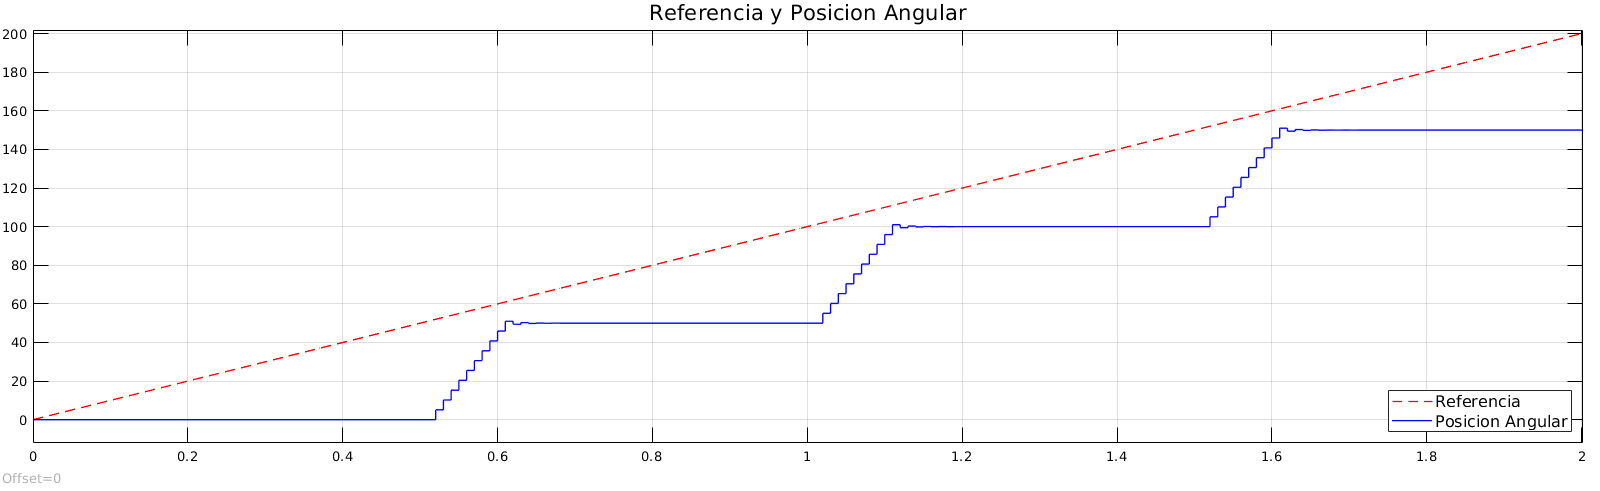
\includegraphics[scale=0.3]{imgmeca/SRD/Sim2_Img2.png}
	\caption{Segunda Simulaci�n. Entrada Rampa. Con aumento. Referencia y Posici�n Angular.}
	\label{img:Sim2_Img2}
\end{figure}

Como se aprecia en la figura \ref{img:Sim2_Img2} el sistema realiza peque�os acercamientos parecidos a escalones, esto debido a la forma de plantear el control pues es a intervalos de $0.5$[s] que el sistema renueva la referencia, generando as� peque�os escalones en la referencia del sistema, sin embargo, el control es realizado a intervalos de $0.01$[s], dando entonces esa apariencia de peque�as respuestas a escalones con desplazamientos en la amplitud.\\

A continuaci�n, en la figura \ref{img:Sim2_Img3}, se expone la din�mica del error a trav�s del tiempo. Se pueden apreciar similitudes con entre las figuras \ref{img:Sim1_Img3} y \ref{img:Sim2_Img3} pues la primera presenta la din�mica del error con respecto a un escal�n, y la segunda presenta la respuesta del sistema con respecto a una rampa tratada como una sucesi�n de escalones, como se explico anteriormente, raz�n por la cual el comportamiento de los errores es parecida.

\begin{figure}[H]
	\centering
	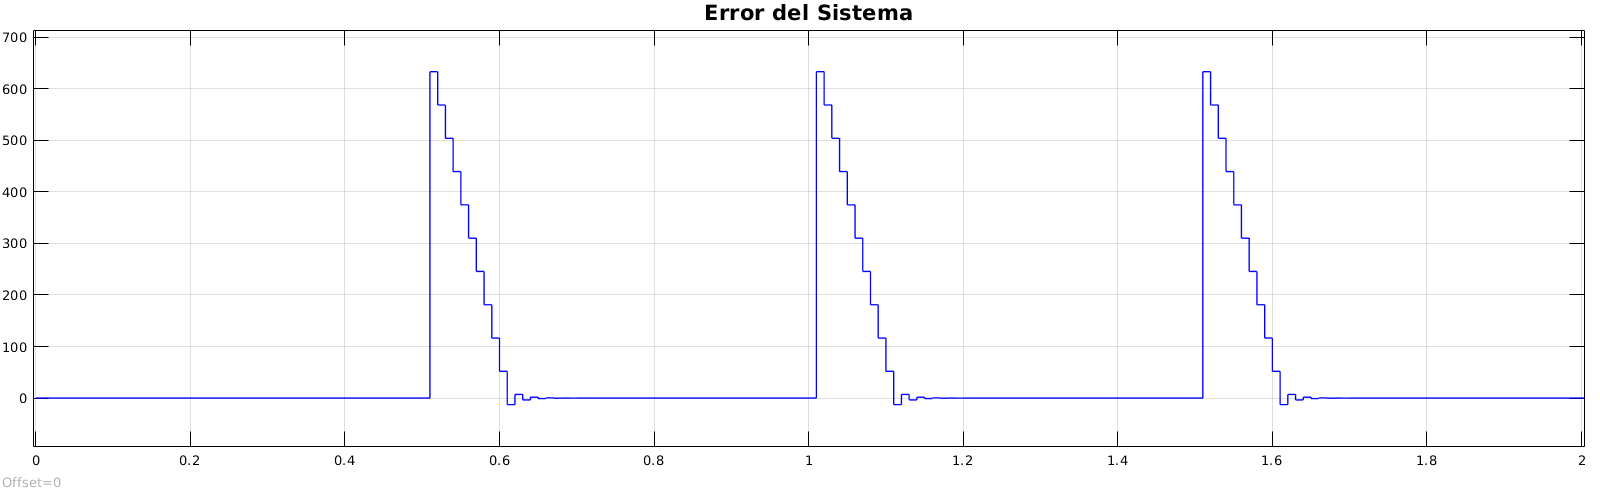
\includegraphics[scale=0.3]{imgmeca/SRD/Sim2_Img3.png}
	\caption{Segunda Simulaci�n. Entrada Rampa. Con aumento. Error del Sistema.}
	\label{img:Sim2_Img3}
\end{figure}


\subsubsection*{Selecci�n de materiales}
Al igual que con el SRVD y el SLVC, los componentes del mecanismo del SRD est�n hechos de aluminio aleaci�n AA 6061 y pl�stico ABS. La base superior, base inferior y el eje est�n hechos de aluminio. En la base inferior hay u rodamiento colocado con ajuste el cual permite el libre giro del eje; por esta raz�n estas piezas se fabricaron de aluminio (imprimirlas en 3D no habr�a permitido un ajuste adecuado entre el rodamiento, la base inferior y el eje).\\

La base del motor, la base de la c�mara y el sujetador de la c�mara fueron impresas en 3D por practicidad y para disminuir la masa del SRD.

}
		
\newpage		
		\subsection{Sistema de Estaci�n en Tierra} \label{sistSET}
% !TeX encoding = ISO-8859-1

{\parindent0pt

El SET se encarga de realizar la comunicaci�n entre el CanSat y la estaci�n en Tierra ($sS_{6{.}1}-$SC-ET), as� como la comunicaci�n entre la estaci�n en Tierra y el usuario ($sS_{6{.}2}-$SU-ET). El SET est� compuesto por la antena y transmisor abordo del CanSat, la antena y el transmisor en Tierra, y la computadora en Tierra ejecutando la interfaz gr�fica de usuario.

			\subsubsection{Subsistema de comunicaci�n CanSat - Estaci�n en Tierra}
El SC-ET lleva a cabo la funci�n $f_{4{.}2}-$\textit{Comunicar con estaci�n en Tierra}.\\

\noindent Una vez que el SCMC haya medido los par�metros externos e internos y el SPD los haya procesado, los datos se env�an por medio de comunicaci�n serial al XBee abordo del CanSat. El XBee abordo del CanSat est� conectado con la antena que se encarga de transmitir la trama de telemetr�a a la estaci�n en Tierra. La tabla \ref{tab:trama} muestra los datos que son transmitidos por el CanSat.

\begin{table}[H]
\begin{center}
\caption{Trama de telemetr�a.}
\label{tab:trama}
\resizebox{14cm}{!}
{
\begin{tabular}{>{\raggedright}p{1cm}>{\raggedright}p{5cm}>{\centering}p{2cm}>{\raggedright}p{8cm}}
\multicolumn{4}{c}{}\tabularnewline
\toprule

\textbf{No.} & \textbf{Par�metro} & \textbf{Ejemplo} & \textbf{Definici�n} \tabularnewline
\midrule

1 & N�mero de paquete & 22 & Indica el n�mero de paquete que se est� transmitiendo $[adim]$.\tabularnewline

2 & Tiempo de misi�n & 11 & Indica el tiempo en que se env�a el paquete $[s]$.\tabularnewline

3 & �ngulo \textit{pitch} & 13.43 & Valor de inclinaci�n alrededor del eje \textit{x} $[grados]$.\tabularnewline

4 & �ngulo \textit{roll} & 23.96 & Valor de inclinaci�n alrededor del eje \textit{y} $[grados]$.\tabularnewline

5 & �ngulo azimut & 108.31 & Valor del GDL de azimut del SRD $[grados]$.\tabularnewline

6 & Presi�n barom�trica & 77823.34 & Valor de presi�n barom�trica de la atm�sfera $[Pa]$.\tabularnewline

7 & Temperatura & 27.49 & Temperatura del aire $[Celsius]$. \tabularnewline

8 & Altura & 325.14 & Estimaci�n de altura con respecto al sitio de lanzamiento $[m]$.\tabularnewline

9 & N�mero de sat�lites (GPS) & 9 & N�mero de sat�lites detectados por el GPS $[adim]$.\tabularnewline

10 & Latitud & 2232.73830 & Valor de latitud otorgado por el GPS $[grados]$.\tabularnewline

11 & Longitud & 11404.58520 & Valor de longitud otorgado por el GPS $[grados]$.\tabularnewline

12 & Altitud & 32908.09 & Valor de altitud otorgado por el GPS con respecto al nivel del mar $[msnm]$.\tabularnewline

13 & Velocidad de rotaci�n del rotor & 325.42 & Velocidad angular de las h�lices $[rpm]$.\tabularnewline

14 & Estado & 3 & Estado actual de la misi�n $[adim]$.\tabularnewline

\bottomrule
\end{tabular}
}
\end{center}
\end{table}

\noindent Los requerimientos especifican que se deben utilizar m�dulos XBee, por lo tanto, se han seleccionado los m�dulos XBee S2 que operan en la banda de frecuencias de 2.4 [GHz]. Habr� un m�dulo tanto abordo del CanSat como en la estaci�n en Tierra.\\

\noindent Los m�dulos XBee S2 operan en la banda de frecuencia ISM $2.4 [GHz]$, que va de $2.4 [GHz]$ a $2.5 [GHz]$, con una frecuencia central de 2.45 [GHz]. Para la selecci�n de la antena a bordo y para el dise�o de la antena en la estaci�n en Tierra se tom� como frecuencia de operaci�n la frecuencia central de $2.45[GHz]$.

\subsubsection*{Antena a bordo del CanSat}
\noindent La antena que va a bordo del CanSat es una antena Taoglas\textsuperscript{\textregistered} [3261A] con $2[dBi]$ de ganancia m�xima con una frecuencia de operaci�n de $2.4[GHz]$ a $2.5[GHz]$. La antena seleccionada posee polarizaci�n circular lo que significa que es apta para aplicaciones donde la orientaci�n del dispositivo en que va montada cambia constantemente.\\

\begin{figure}[H]
	\centering
		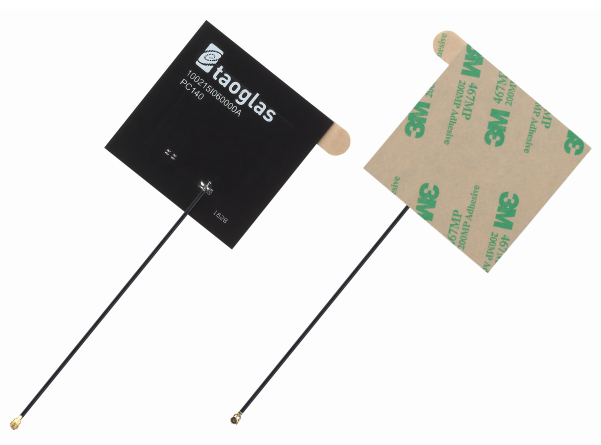
\includegraphics[scale=0.5]{diseniosist/SET/taoglas}
	\caption{Antena a bordo del CanSat.}
	\label{img:taoglas}
\end{figure}

\noindent La ganancia de una antena hace referencia a qu� tan bien la antena convierte la potencia el�ctrica en ondas de radio y viceversa [?]. La imagen \ref{img:GainTaoglas} muestra el valor de ganancia de la antena a bordo del CanSat en un rango de frecuencia de $2.3 [GHz]$ a $2.6 [GHz]$. En la imagen \ref{img:GainTaoglas} se puede observar que la ganancia de la antena a una frecuencia de $2.45 [GHz]$ es aproximadamente de $1.55 [dBi]$.\\

\noindent Otro par�metro importante de una antena es la Raz�n de Onda Estacionaria (\textit{Voltage Standing Wave Ratio}, VSWR). El par�metro VSWR es una medida de la cantidad de potencia que se entrega a la antena en comparaci�n con la cantidad de potencia que se refleja de la antena. Cada antena tiene un valor caracter�stico de impedancia, y el cable que la conecta con el transmisor tambi�n lo tiene. El caso ideal ocurre cuando ambos elementos (antena y cable) poseen la misma impedancia; cuando esto sucede, el valor del par�metro VSWR es de 1.  En la pr�ctica, se toma un valor del par�metro VSWR de 2 como el m�ximo permisible.\\

\begin{figure}[H]
	\centering
		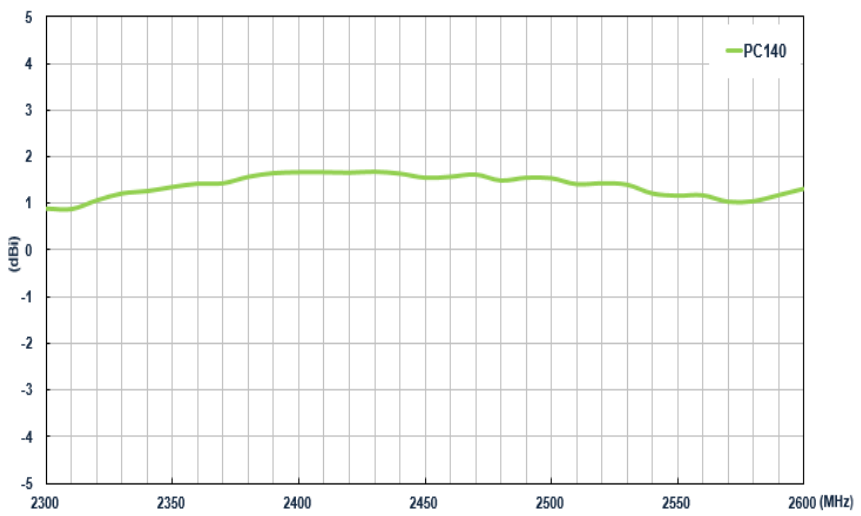
\includegraphics[scale=0.5]{diseniosist/SET/gain}
	\caption{Ganancia de la antena a bordo del CanSat.}
	\label{img:GainTaoglas}
\end{figure}


\noindent La imagen \ref{img:VSWRTaoglas} muestra el valor del par�metro VSWR de la antena a bordo del CanSat para un rango de frecuencias de $2.0 [GHz]$ a $3.0 [GHz]$. Como se observa en la imagen \ref{img:VSWRTaoglas} el valor del par�metro VSWR para una frecuencia de $2.45 [GHz]$ es menor a 2.

\begin{figure}[H]
	\centering
		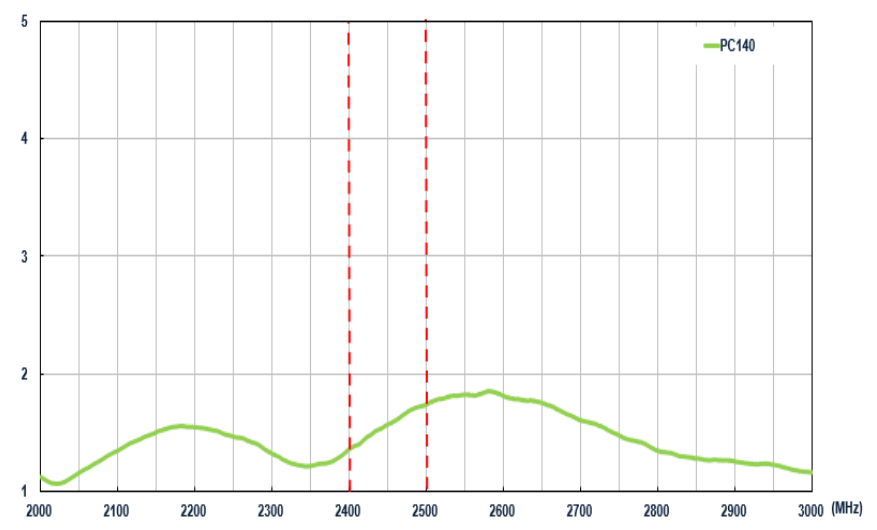
\includegraphics[scale=0.5]{diseniosist/SET/taoglasVSWR}
	\caption{Par�metro VSWR de la antena a bordo del CanSat.}
	\label{img:VSWRTaoglas}
\end{figure}

\noindent Los patrones de radiaci�n son otro par�metro importante de una antena. El patr�n de radiaci�n de una antena es una representaci�n gr�fica de la energ�a irradiada por la antena en funci�n del espacio [?]. El patr�n de radiaci�n describe la forma en que la antena irradia energ�a en el espacio.\\

\noindent La imagen \ref{img:taoglasradpat} muestra los patrones de radiaci�n de la antena a bordo del CanSat en los planos \textit{xy} (arriba izquierda), \textit{xz} (arriba derecha) y \textit{yz} (abajo izquierda). Tambi�n se muestra el patr�n de radiaci�n en un plano 3D (abajo derecha). En la imagen \ref{img:taoglasradpat} se observa que la antena se comporta como una antena omnidireccional, es decir, como una antena en que la radiaci�n de ondas no se concentra en una sola direcci�n, sino que se distribuye por todo el espacio. Esto es particularmente �til para la antena de abordo puesto que permitir� que haya comunicaci�n continua entre el CanSat y la estaci�n en Tierra independientemente de la orientaci�n que el CanSat adquiera durante el vuelo.


\begin{figure}[H]
	\centering
		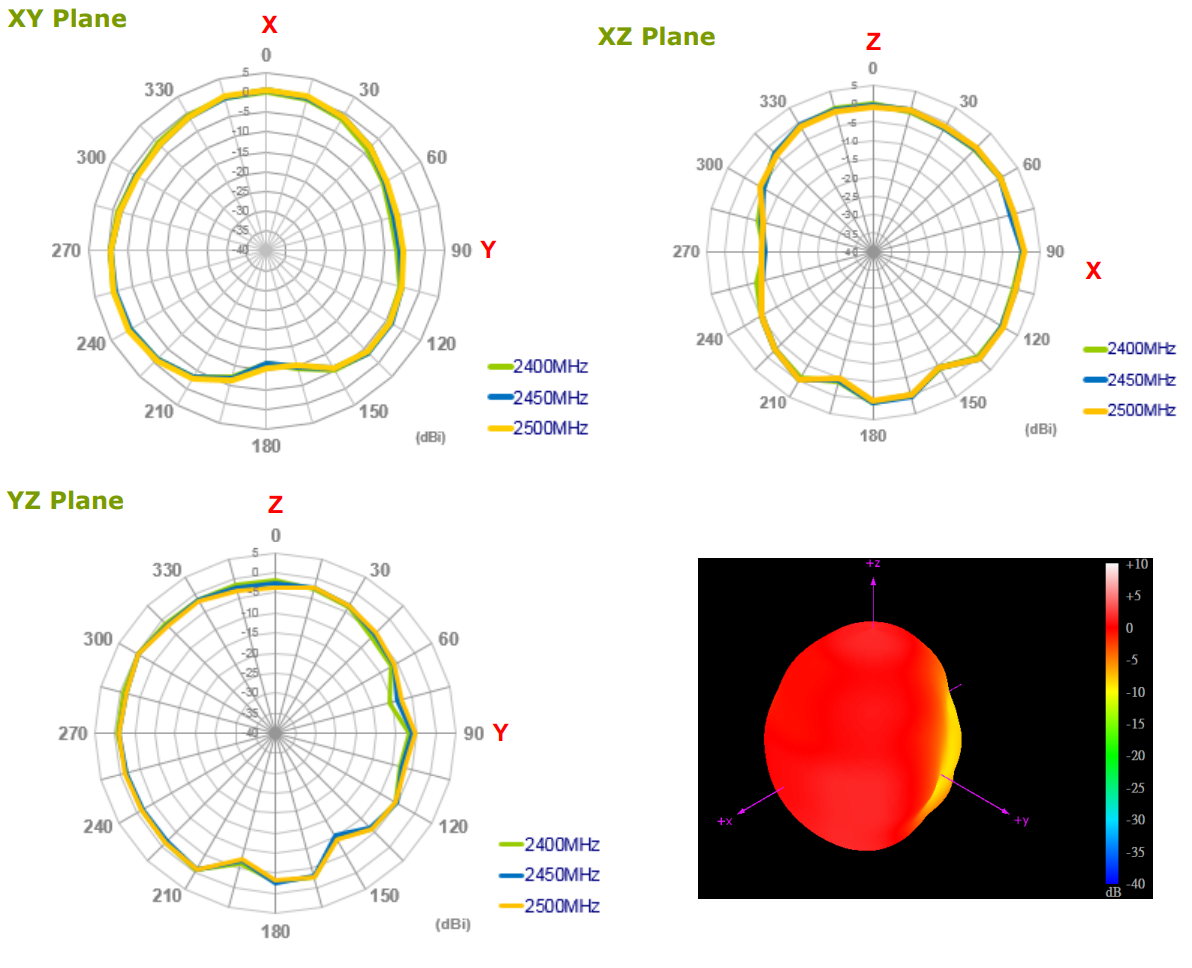
\includegraphics[scale=0.45]{diseniosist/SET/taoglasradi}
	\caption{Patrones de radiaci�n de la antena a bordo del CanSat (en los planos \textit{xy}, \textit{xz} y \textit{yz}, y en 3D).}
	\label{img:taoglasradpat}
\end{figure}


\subsubsection*{Antena en Tierra}
La antena para la estaci�n en Tierra es una antena BiQuad. La antena BiQuad es port�til (puede ser sostenida con la mano). Como se mostrar� m�s adelante, la antena posee un amplio patr�n de radiaci�n lo que elimina la necesidad de apuntarla en una direcci�n muy espec�fica (la ruta en el aire que seguir� el CanSat es impredecible, por lo que es importante que la antena en Tierra pueda cubrir una zona m�s amplia para mantener la comunicaci�n).\\

\begin{figure}[H]
	\centering
		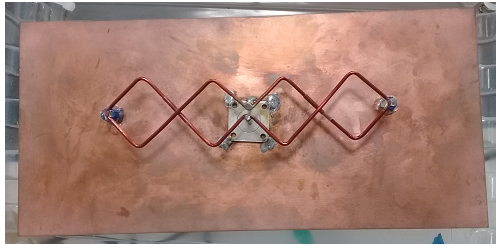
\includegraphics[scale=0.70]{diseniosist/SET/antenaBiQuadcompleta}
	\caption{Antena BiQuad de la estaci�n en Tierra.}
	\label{img:BiQuad}
\end{figure}

\noindent La imagen \ref{img:dimBiQuad} muestra las dimensiones de una antena BiQuad. Para el caso de la antena construida para la estaci�n en Tierra se tiene que $RL = 280[mm]$, $RH = 135[mm]$, $EL = 165[mm]$, $ED = 30[mm]$, $D = 40[mm]$ y $S = 20[mm]$. Para el reflector se utiliz� una placa de cobre. Para los rombos se utiliz� alambre de cobre de $3 [mm]$ de di�metro. Finalmente, el cable coaxial est� conectado a los rombos.\\

\begin{figure}[H]
	\centering
		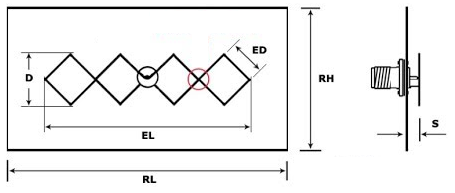
\includegraphics[scale=0.95]{diseniosist/SET/dimquad}
	\caption{Dimensiones de la antena BiQuad.}
	\label{img:dimBiQuad}
\end{figure}

\noindent La antena BiQuad con estas dimensiones y estos materiales se simul� en el programa ANSYS--HSSF\textregistered para obtener los valores de ganancia, VSWR y los patrones de radiaci�n.\\

\noindent La imagen \ref{img:GainBQ} muestra los valores de ganancia de la antena BiQuad para un rango de frecuencias de $2.02 [GHz]$ a $2.85 [GHz]$. La imagen \ref{img:GainBQ} muestra que la ganancia de la antena BiQuad es de $12.6759 [dBi]$ a una frecuencia de $2.45 [GHz]$, que se ubica en la zona cerca del m�ximo de la gr�fica. Este valor de ganancia es mucho mayor al de la ganancia de la antena a bordo.\\

\begin{figure}[H]
	\centering
		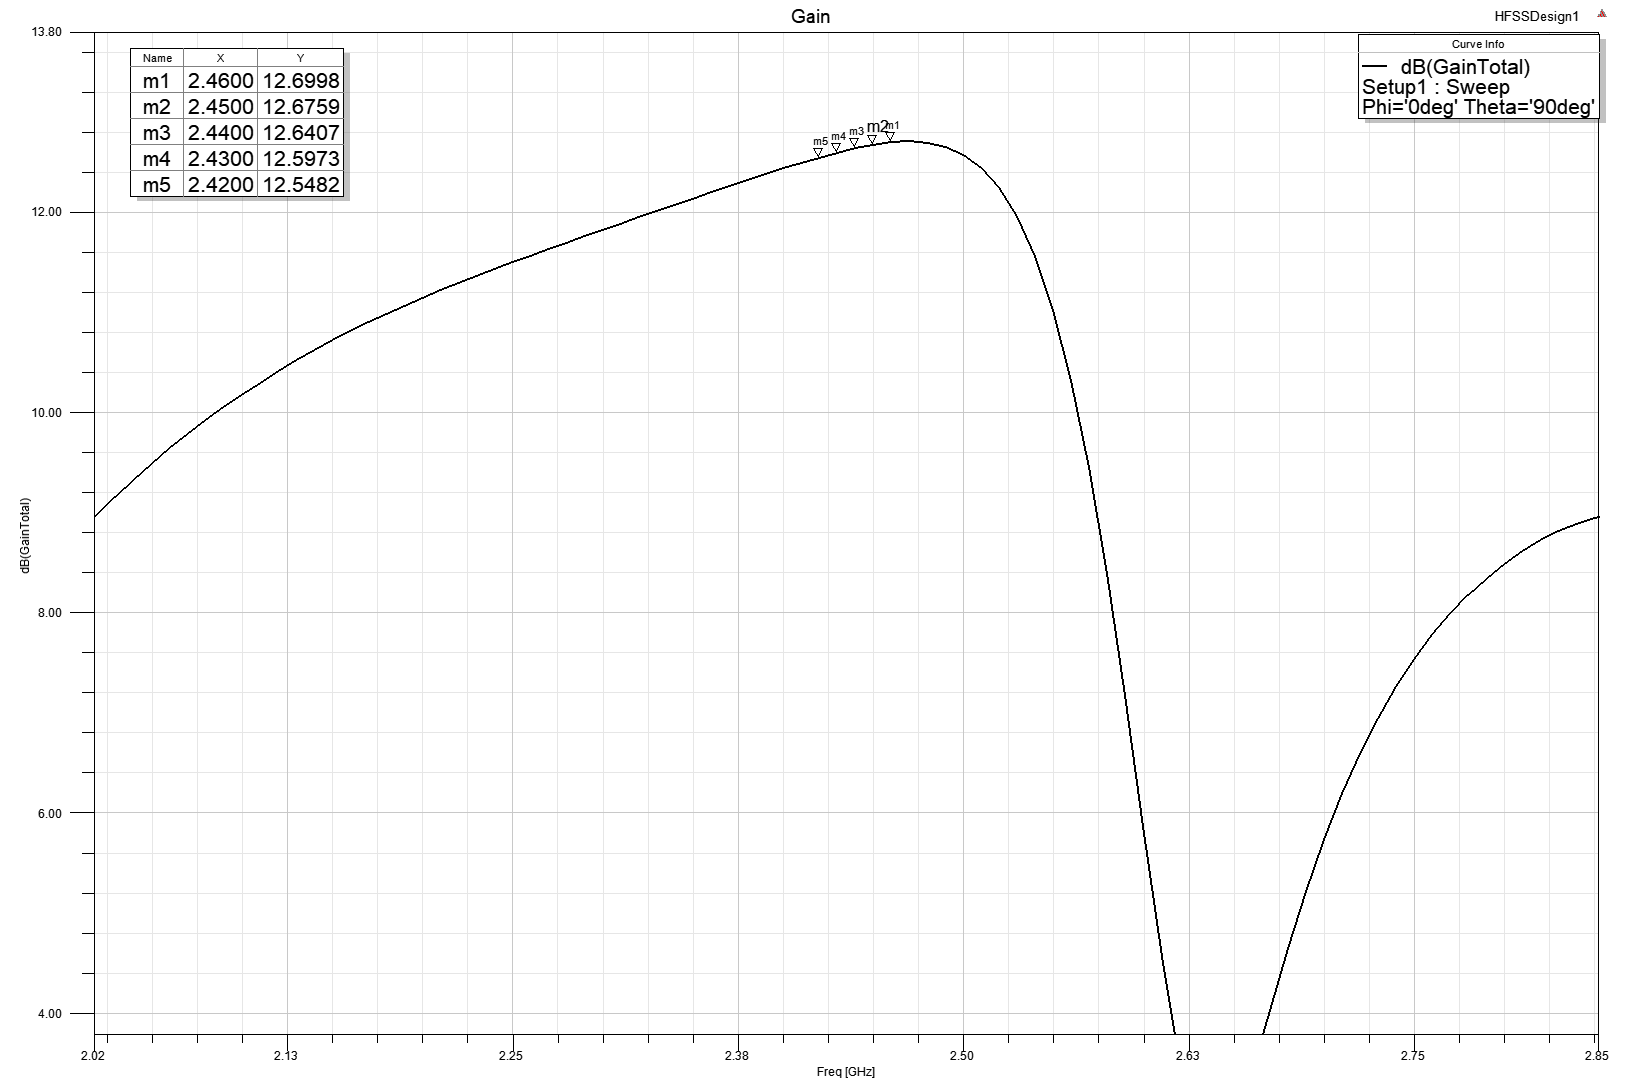
\includegraphics[scale=0.20]{diseniosist/SET/BiQuadGain}
	\caption{Ganancia de la antena BiQuad.}
	\label{img:GainBQ}
\end{figure}

\noindent La imagen \ref{img:VSWRBQ} muestra los valores del par�metro VSWR de la antena BiQuad. Se observa que a una frecuencia de $2.45 [GHz]$ el par�metro VSWR tiene un valor de $1.7001$, que se ubica por debajo del m�ximo permisible.\\

\begin{figure}[H]
	\centering
		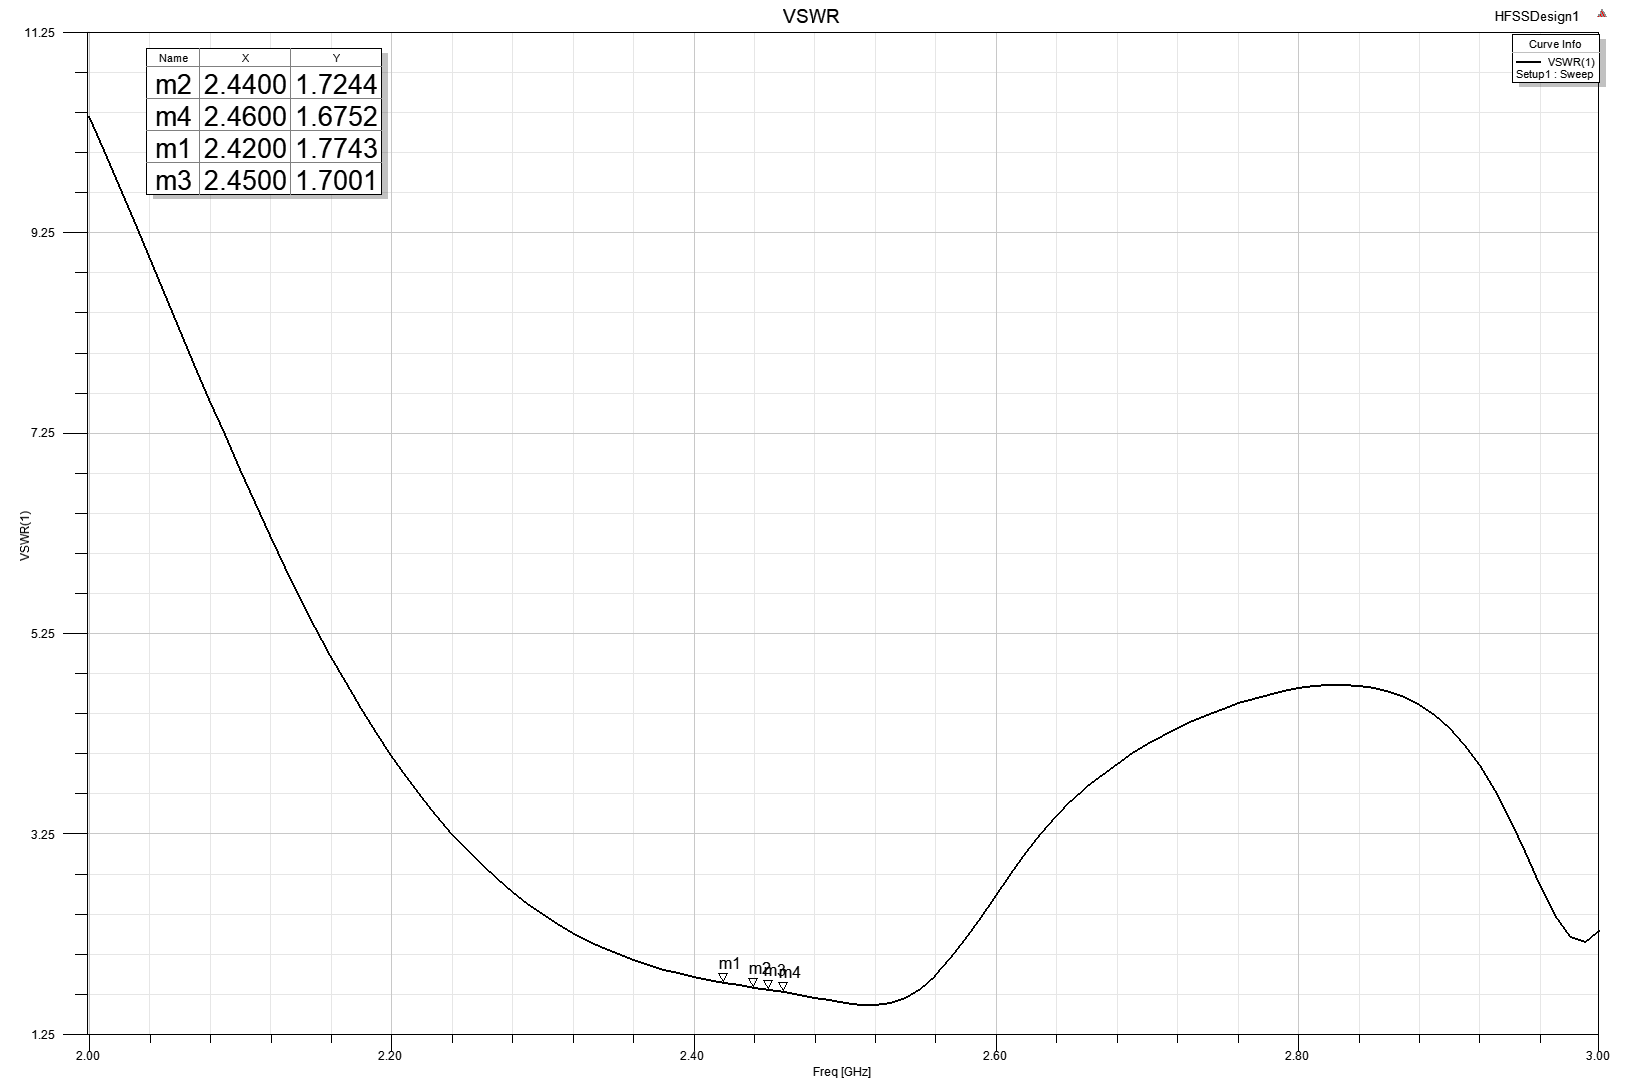
\includegraphics[scale=0.20]{diseniosist/SET/VSWR}
	\caption{Par�metro VSWR de la antena BiQuad.}
	\label{img:VSWRBQ}
\end{figure}

\noindent La imagen \ref{img:patradbi} muestra los patrones de radiaci�n en los planos \textit{xy} (izquierda arriba) y \textit{xz} (derecha arriba), as� como el patr�n de radiaci�n en 3D (centro abajo) de la antena BiQuad.\\

\noindent La imagen \ref{img:patradbi} muestra que la antena BiQuad tiene un l�bulo preponderante en la parte frontal. La imagen \ref{img:patradbi} muestra que el comportamiento del patr�n de radiaci�n de la antena BiQuad es muy similar para valores de frecuencia de $2.42 [GHz]$, $2.44 [GHz]$, $2.45[GHz]$ y $2.46 [GHz]$.\\

\noindent De los patrones de radiaci�n de la antena BiQuad se puede concluir que la antena tendr� una amplia cobertura para recibir se�ales provenientes del CanSat, a pesar de que �ste siga una ruta impredecible durante el vuelo. Lo anterior permitir� sostener la antena con la mano sin la necesidad de apuntarla tanto hacia el CanSat.\\

\begin{figure}[H]
	\centering
		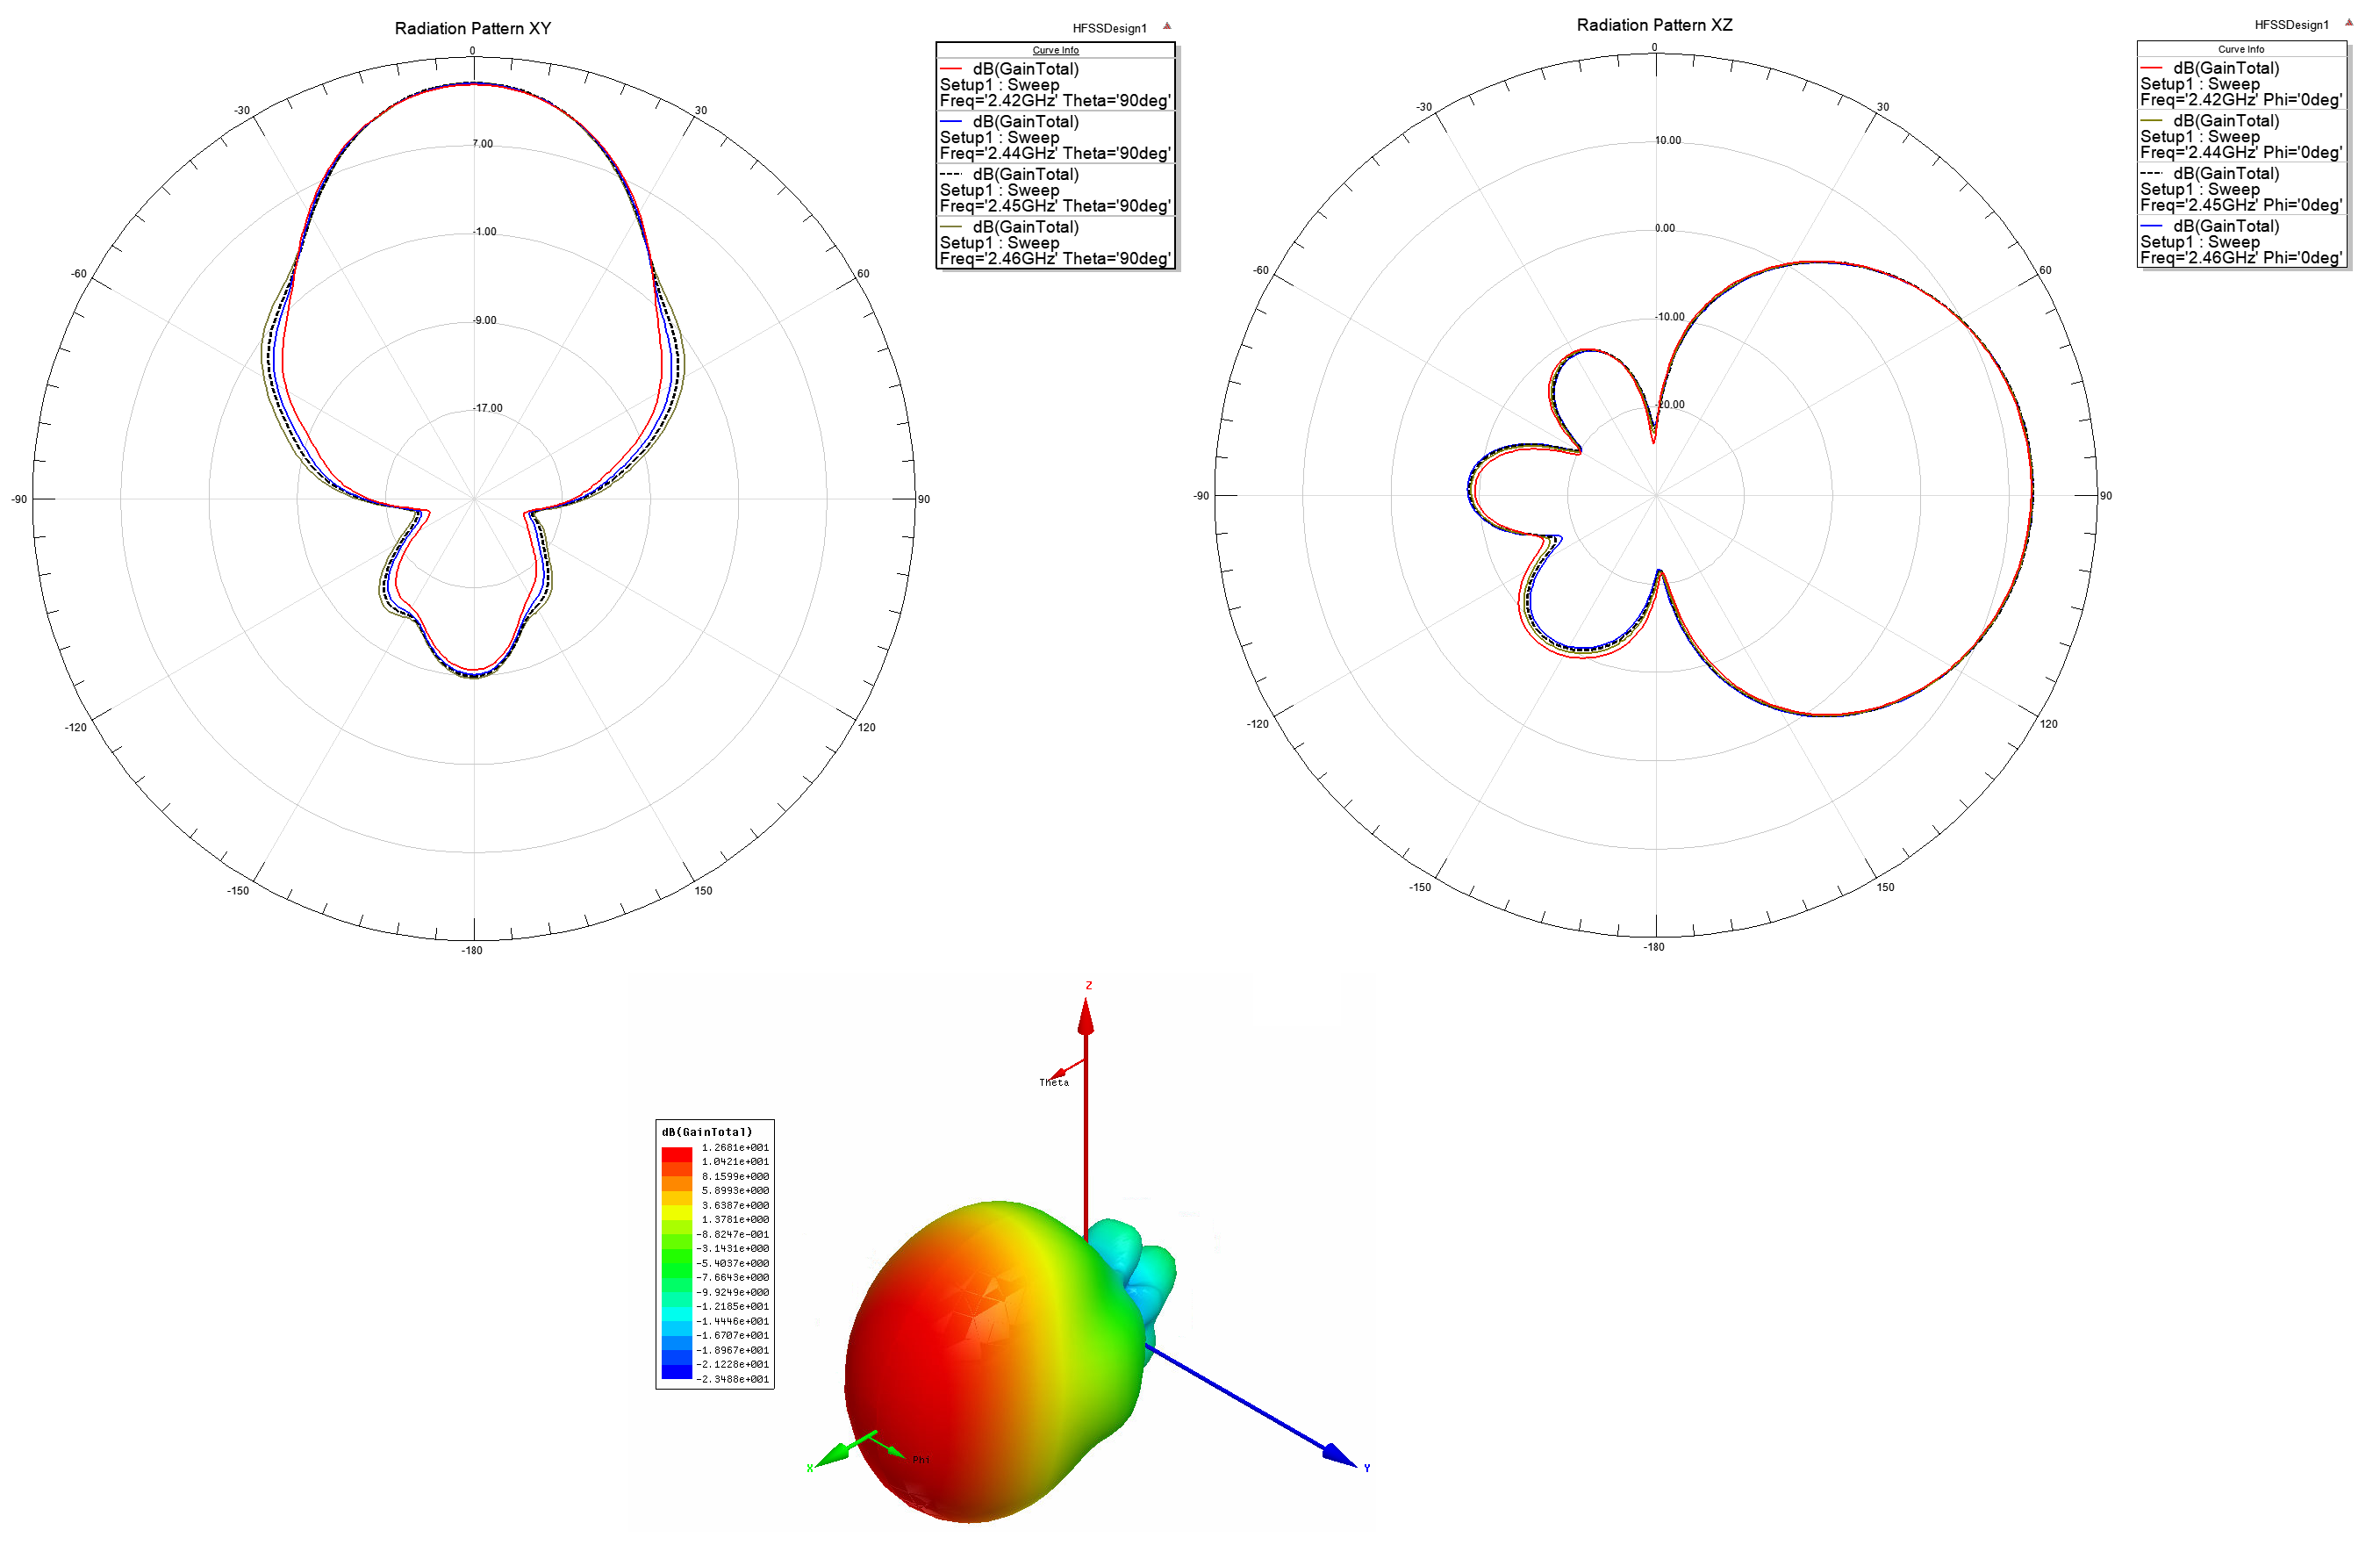
\includegraphics[scale=0.2]{diseniosist/SET/radpatbiquad}
	\caption{Patrones de radiaci�n de la antena BiQuad.}
	\label{img:patradbi}
\end{figure}


			\subsubsection{Subsistema de comunicaci�n Usuario - Estaci�n en Tierra}
El SU-ET lleva a cabo la funci�n $f_{2{.}1{.}2}-$\textit{Almacenar datos} y $f_{2{.}1{.}4}-$\textit{Interactuar con el usuario}.\\

\noindent El SU-ET toma la trama de datos recibida por la antena BiQuad y la despliega en pantalla para que el usuario pueda visualizar los datos. Para lograr dicha visualizaci�n se desarroll� una interfaz gr�fica de usuario (IGU). La IGU se desarroll� utilizando el languaje de programaci�n Python [3262A] y la paqueter�a PyQt5 [3262B].\\

\noindent La IGU de la estaci�n en Tierra posee tres ventanas con las que el usuario inetract�a: ventana de configuraci�n, ventana de monitoreo y ventana de visualizaci�n.

\subsubsection*{Ventana de configuraci�n}
La ventana de configuraci�n se muestra en la figura \ref{img:configwin}. La ventana de configuraci�n posee dos secciones: `Archivo .csv' y `Comunicaci�n serial'. En la secci�n `Archivo .csv' el usuario puede especificar el nombre del archivo \textit{.csv} donde se almacenar�n los datos enviados por el CanSat y el directorio donde se guardar� este archivo. En la secci�n `Comunicaci�n serial' el usuario puede seleccionar el puerto serial al que est� conectado el XBee de la antena BiQuad.\\

\begin{figure}[H]
	\centering
		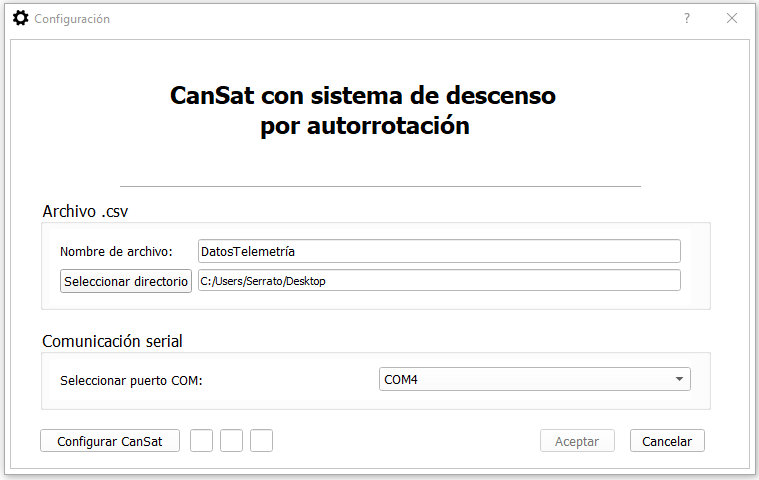
\includegraphics[scale=0.70]{diseniosist/SET/configwindow}
	\caption{Ventana de configuraci�n.}
	\label{img:configwin}
\end{figure}

\noindent La ventana de configuraci�n no permite que el usuario pase a la siguiente ventana, la ventana de monitoreo, hasta que se realice la configuraci�n inicial del CanSat. Esta configuraci�n inicial del CanSat se realiza al presionar el bot�n `Configurar CanSat' ubicado en la esquina inferior izquierda de la ventana.\\

\noindent Cuando el usuario presiona el bot�n `Configurar CanSat' la interfaz env�a al CanSat los comandos \texttt{M,G,------}, \texttt{M,A,------} y \texttt{M,S,------} para calibrar el giroscopio, el aceler�metro y establecer la altura de referencia, respectivamente. Si la configuraci�n resulta exitosa el bot�n `Aceptar' se habilita, permitiendo al usuario continuar a la ventana de monitoreo. De resultar una configuraci�n fallida el bot�n `Aceptar' queda deshabilitado hasta que la configuraci�n sea exitosa. En ambos casos se manda un mensaje informativo al usuario.\\

\noindent As� mismo, la interfaz muestra mensajes de error en caso de que alg�n campo quede faltante (nombre de archivo, directorio o puerto COM) o el nombre de archivo o directorio tenga un caracter no permitido. El usuario puede cerrar la ventana de configuraci�n en cualquier momento con el bot�n `Cancelar'.\\

\noindent Al momento de presionar el bot�n `Aceptar' la interfaz manda el comando \texttt{B,S,------} para indicarle al CanSat que comience con la transmisi�n de datos.

\subsubsection*{Ventana de monitoreo}
La ventana de monitoreo se muestra en la figura \ref{img:monitorwin}. La ventana de monitoreo posee cuatro secciones: `Informaci�n de la misi�n', `Datos de GPS', `Datos de telemetr�a' y �rea de graficaci�n.\\

\noindent En la secci�n de `Informaci�n de la misi�n' se muestra la trama de datos completa recibida por la estaci�n en Tierra, el n�mero de paquete recibido, el tiempo actual de la misi�n en segundos, y el estado actual de la misi�n (espera, ascenso, paraca�das, autorrotaci�n y aterrizaje). En la secci�n `Datos de GPS' se muestran los par�metros de latitud, longitud, altitud y n�mero de sat�lites, mientras que en la secci�n `Datos de telemetr�a' se muestran los datos de altura, presi�n atmosf�rica, temperatura, velocidad del rotor, �ngulo \textit{pitch}, �ngulo \textit{roll} y �ngulo \textit{azimuth}. Finalmente, en el �rea de graficaci�n se despliegan los ejes de altura, presi�n, temperatura, velocidad del rotor, orientaci�n (\textit{pitch}, \textit{roll} y \textit{azimuth}) y GPS (latitud contra longitud).\\

\noindent El usuario debe presionar el bot�n `Iniciar' para que la ventana de monitoreo comience a desplegar los datos en pantalla (recordar que para este punto el CanSat ya est� transmitiendo los datos). Cuando el CanSat ha aterrizado la ventana de monitoreo detiene el despliegue de datos y habilita el bot�n de `Continuar'. El bot�n de `Continuar' cierra la ventana de monitoreo y abre la ventana de visualizaci�n. En cualquier momento el usuario puede cerrar la ventana de monitoreo al presionar el bot�n `Terminar'.\\

\begin{figure}[H]
	\centering
		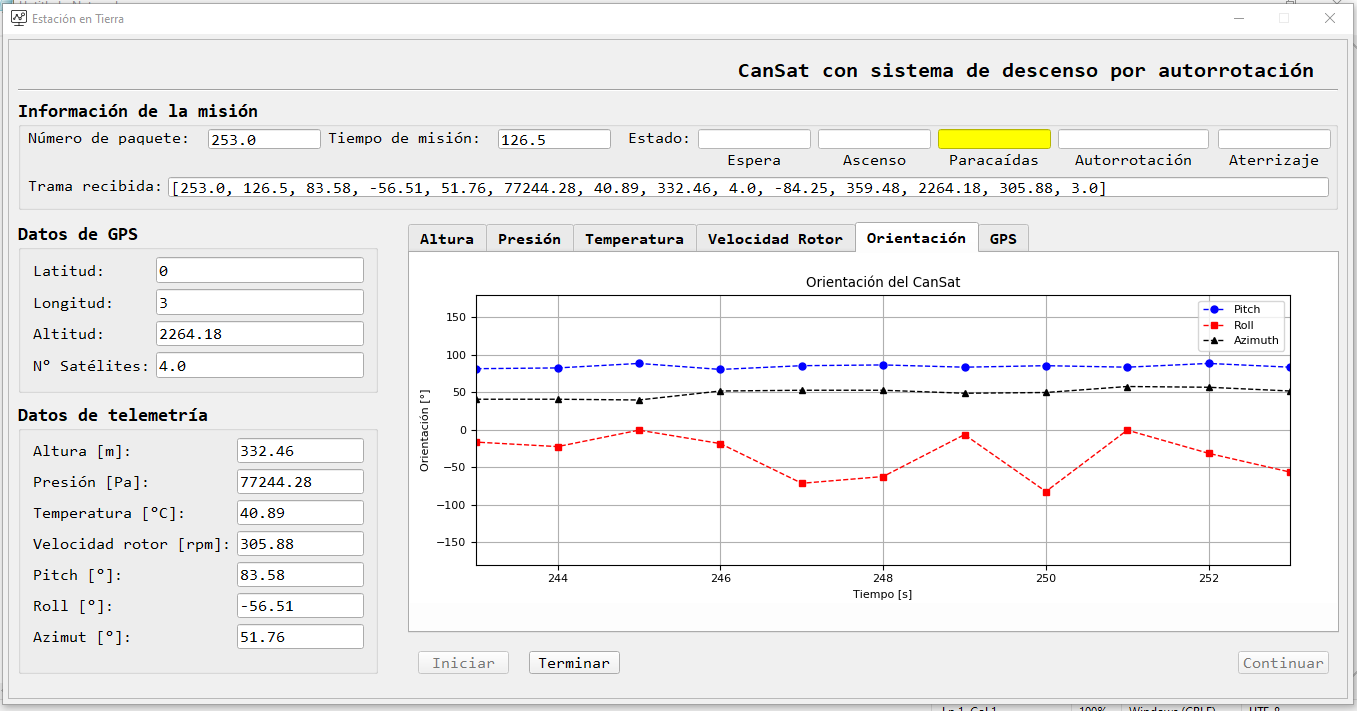
\includegraphics[angle = -90, scale=0.55]{diseniosist/SET/monitorwindow}
	\caption{Ventana de monitoreo.}
	\label{img:monitorwin}
\end{figure}

\subsubsection*{Ventana de visualizaci�n}
La ventana de visualizaci�n se muestra en la figura \ref{img:visualwin}. En la ventana de visualizaci�n el usuario puede ver los datos almacenados en el archivo \textit{.csv} durante la misi�n. En esta ventana el usuario puede seleccionar el par�metro que desea ver y manipular la gr�fica: realizar acercamientos, desplazamientos y guardar la imagen.

\begin{figure}[H]
	\centering
		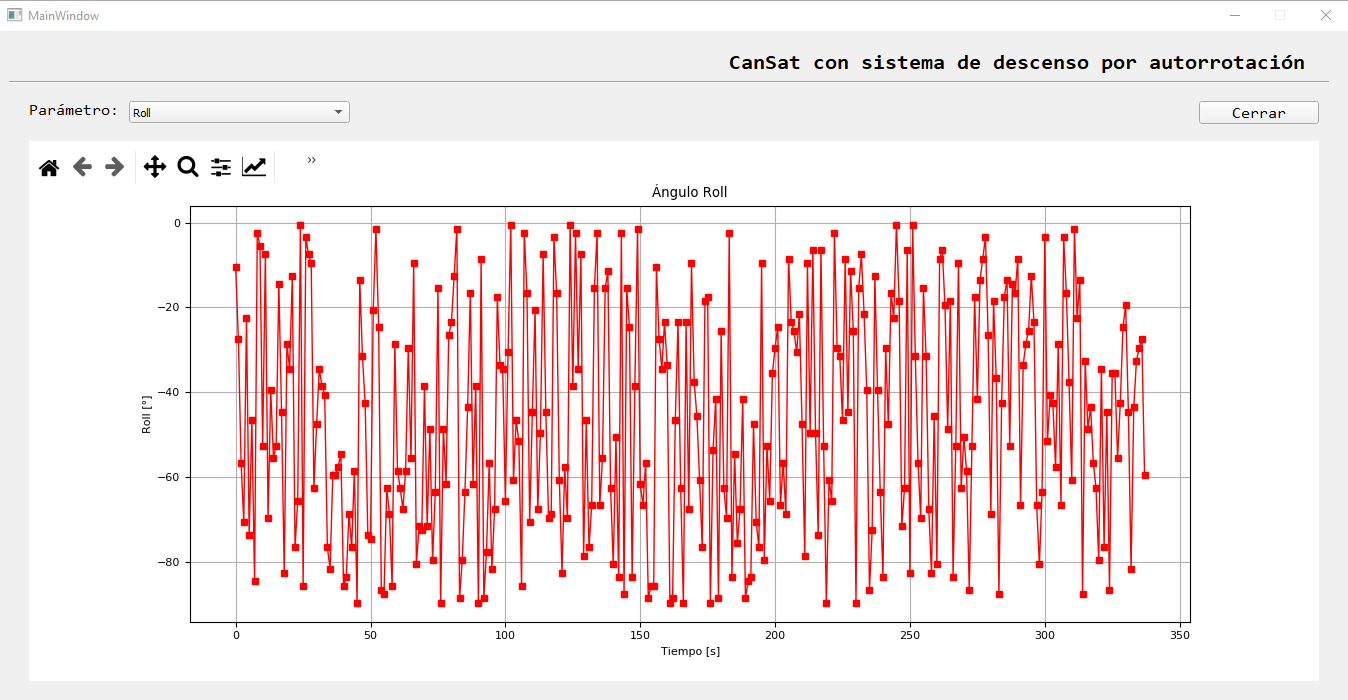
\includegraphics[scale=0.4]{diseniosist/SET/seewindow}
	\caption{Ventana de visualizaci�n.}
	\label{img:visualwin}
\end{figure}

\subsubsection*{Multiprocesos}
El proceso de recepci�n y graficaci�n de datos en la interfaz en Tierra se puede realizar de varias maneras. En un enfoque la interfaz recibir�a la trama de datos enviada por el CanSat, despu�s la segmentar�a para extraer los datos individuales, y finalmente canalizar�a cada uno a su destino (una gr�fica, un recuadro u otro indicador gr�fico). El proceso anterior se desarrollar�a secuencialmente. En este enfoque surge el problema de que la interfaz no podr�a recibir m�s tramas de datos hasta que el proceso de graficaci�n terminara. Lo anterior podr�a causar que varias tramas de datos se perdieran, especialmente si la frecuencia de transmisi�n es alta.\\

\noindent Para resolver este problema los procesos de recepci�n de datos y de graficaci�n deber�an ser independientes uno del otro, pero mantener un canal de comunicaci�n entre ellos. Un enfoque de multiprocesos cumple con estas caracter�sticas. La IGU desarrollada para la estaci�n en Tierra se desarroll� bajo este concepto.\\

\noindent La figura \ref{img:multipro} muestra el dise�o de la interfaz bajo el enfoque de multiprocesos.

\begin{figure}[H]
	\centering
		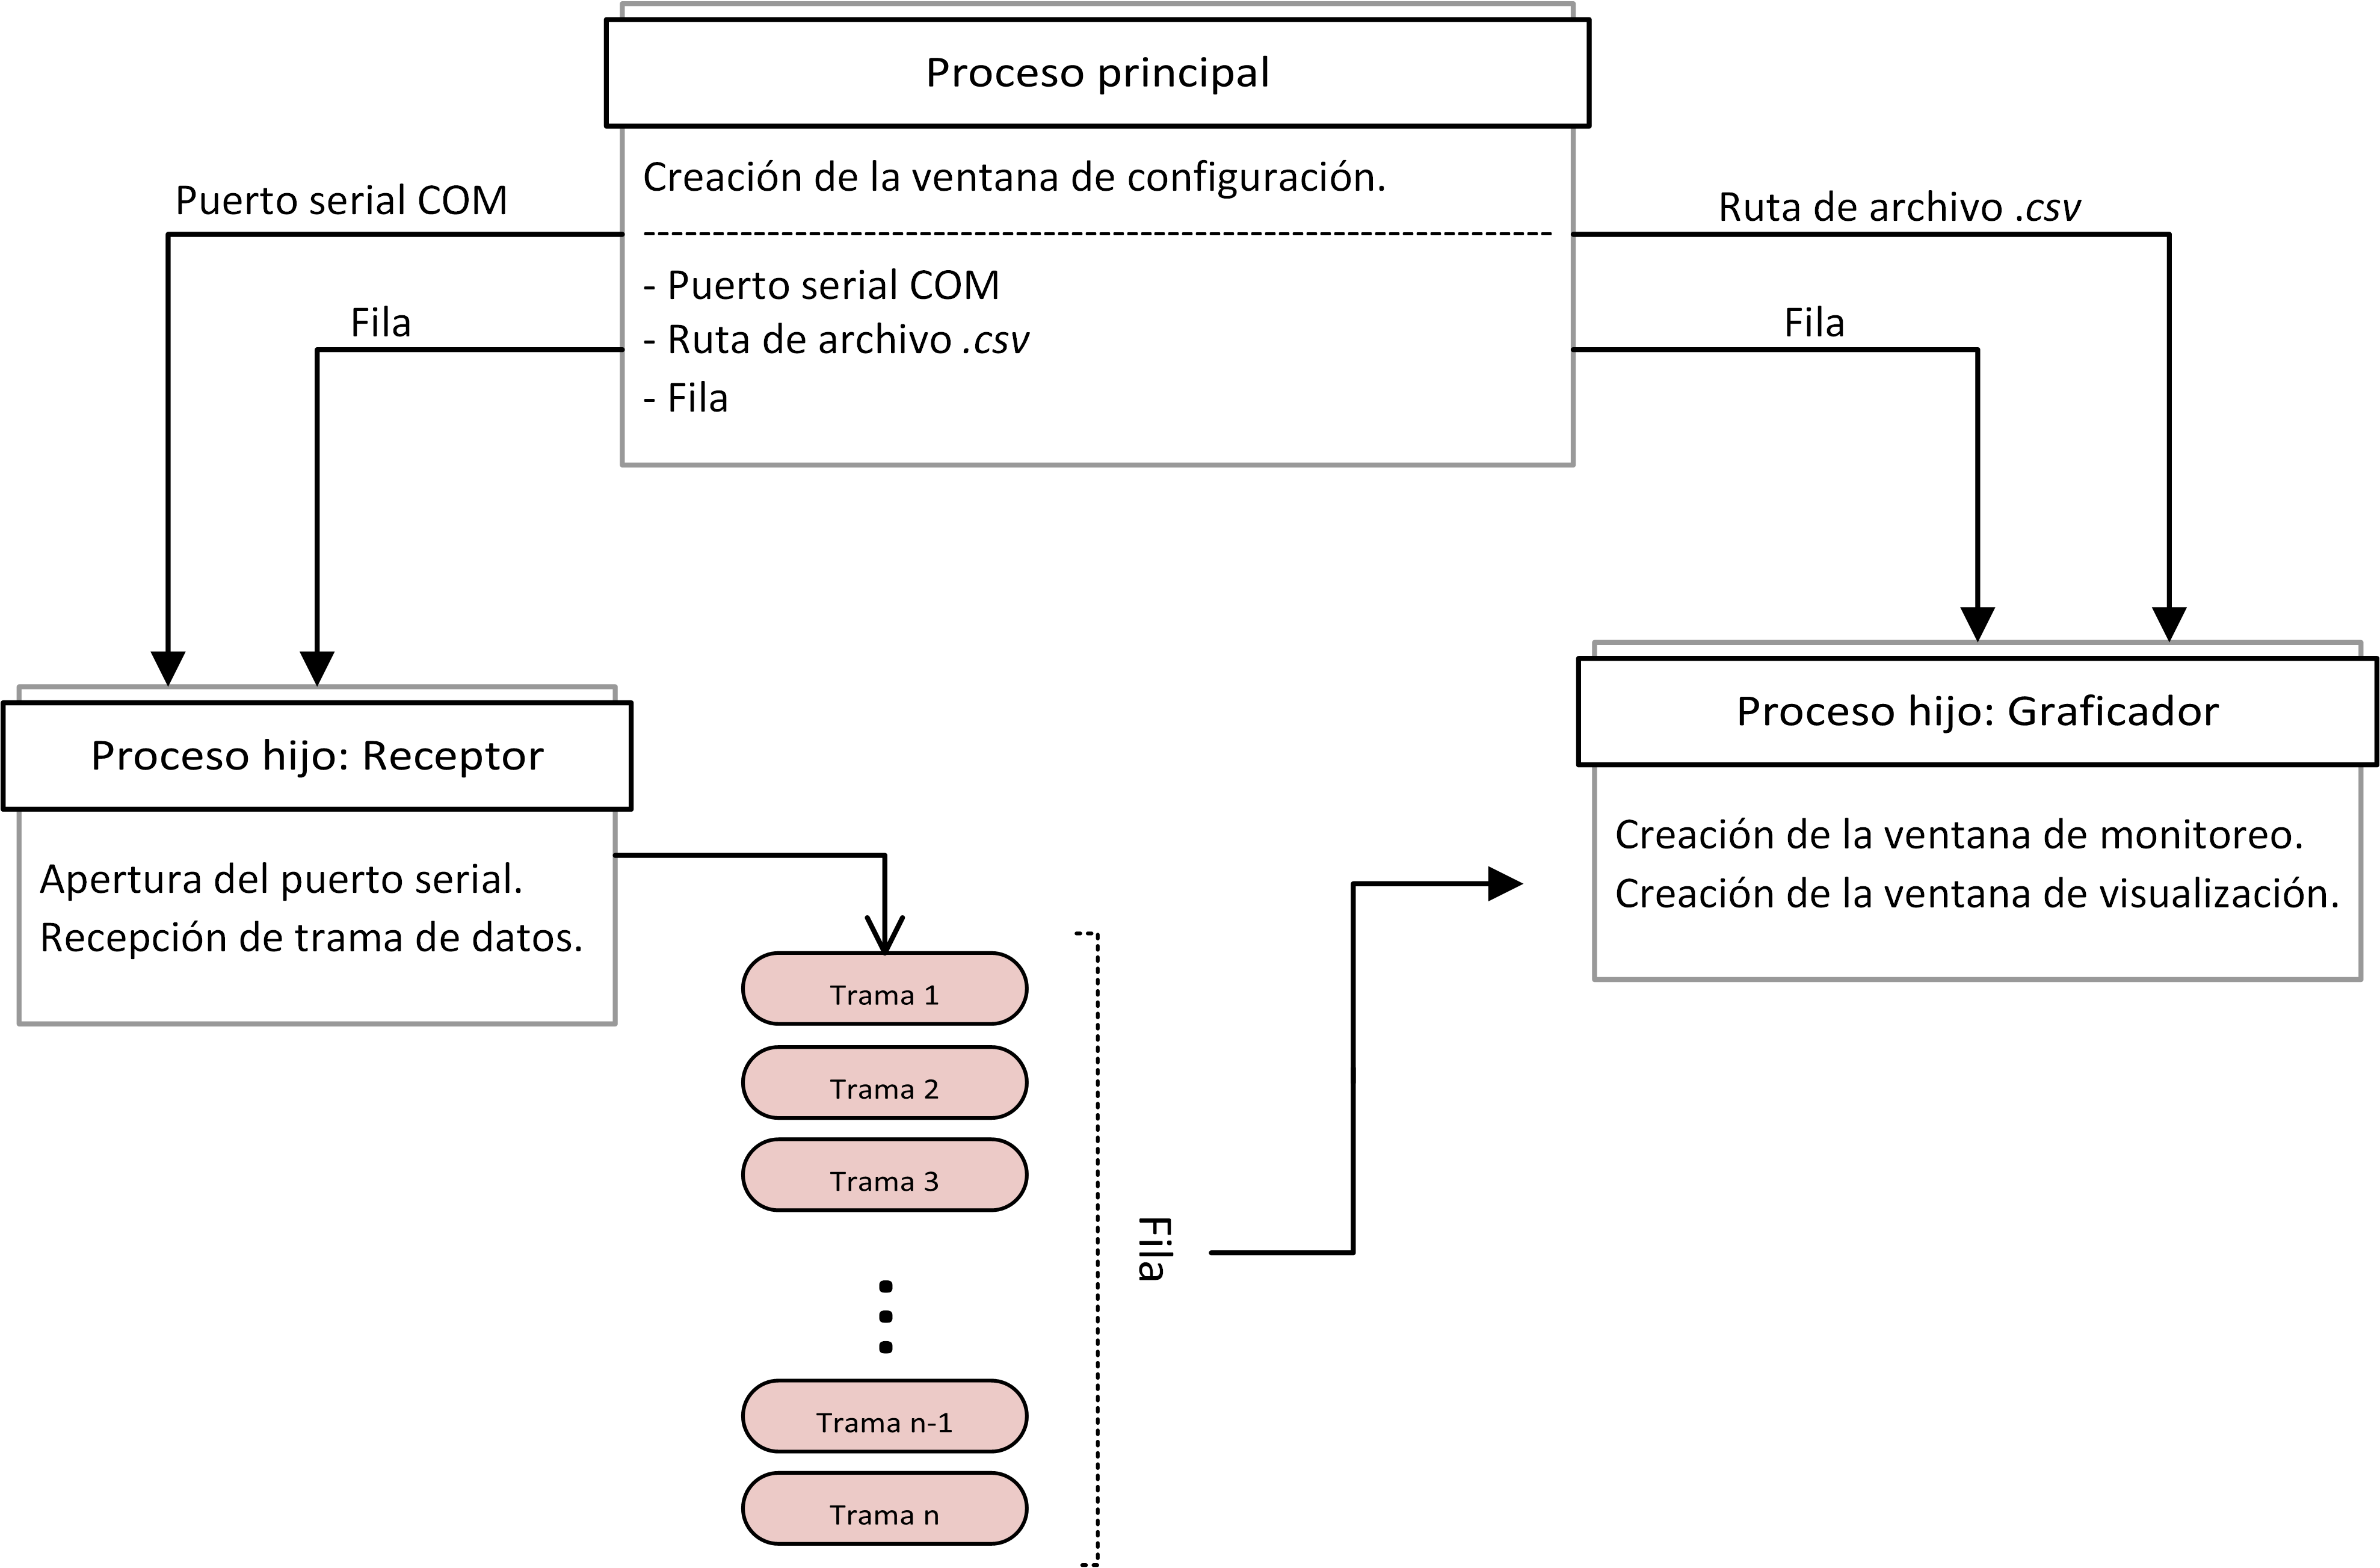
\includegraphics[scale=0.75]{diseniosist/SET/multiprocess}
	\caption{Dise�o de la IGU bajo el enfoque de multiprocesos.}
	\label{img:multipro}
\end{figure}

\noindent En el proceso principal se ejecuta la ventana de configuraci�n. Cuando la participaci�n de la ventana de configuraci�n termina (al momento en que el usuario presiona el bot�n `Aceptar') se crean los dos procesos hijos: los procesos receptor y graficador. En ese momento ambos procesos corren en paralelo; tienen recursos computacionales independientes. Lo anterior permite distribuir la carga de trabajo entre dos n�cleos de la computadora, mejorando el desempe�o de la interfaz.\\

\noindent La forma en que se comunican ambos procesos hijos es mediante la utilizaci�n de filas (\textit{queues}). Python posee un m�dulo para desarrollar c�digo utilizando multiprocesos y filas.\\

\noindent Debido a que el proceso Receptor es independiente del proceso Graficador, el CanSat puede enviar tramas de datos a una frecuencia mayor a la que el proceso Graficador utiliza para desplegar los datos en pantalla. Para el proyecto el CanSat env�a una trama de datos cada $0.5 [s]$, lo que significa que el proceso Receptor recibir� 2 tramas cada segundo y las pondr� en la fila. El proceso Graficador est� programado para actualizar los datos en pantalla cada segundo. De esta manera, cuando se actualicen los datos en pantalla, se tomar�n todos los datos que hasta ese momento se hayan acumulado en la fila.\\

}

\newpage
		\subsection{Sistema de Energ�a} \label{sistSEn}
El Sistema de Energ�a se encarga de almacenar, distribuir y acondicionar la energ�a el�ctrica para todos los componentes del CanSat. Se debe tener en cuenta que dentro del CanSat existe una cantidad considerable de dispositivos electr�nicos como sensores, indicadores, motores, entre otros, los cuales tienen la finalidad de trabajar en conjunto para cumplir los requerimientos de la misi�n. Estos dispositivos trabajan a diferentes niveles de tensi�n, por lo que se debe asegurar que �ste sea el adecuado para cada uno.\\

\noindent En la figura \ref{fig:DiagramaCansat} se presentan los componentes relacionados con las distribuci�n y acondicionamiento de energ�a en el CanSat. El MOSFET de canal P tiene la finalidad de proteger el circuito el�ctrico de una polarizaci�n inversa (conectar las terminales de la bater�a al rev�s). Como se puede ver en la figura \ref{fig:DiagramaCansat}, el voltaje de entrada al CanSat es de $ 9 [V] $ y, al pasar por toda la circuiter�a respectiva, se producen dos salidas de tensi�n: una a $6 [V]$ y la otra a $3.3 [V]$.

\begin{figure}[H]
\begin{center}
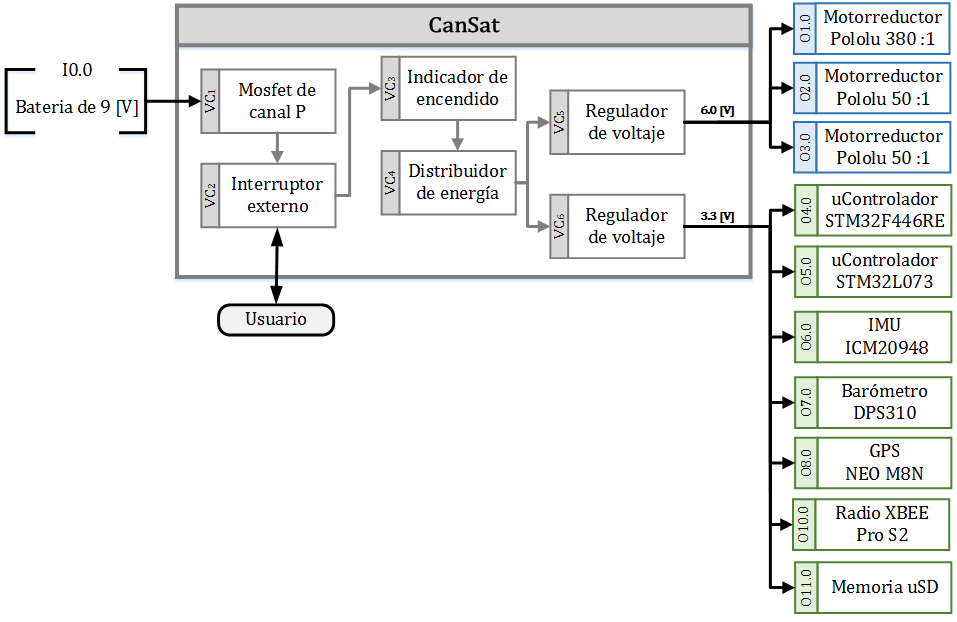
\includegraphics[scale=0.5]{diseniosist/SEn/DiagramaCansat.png}  
\caption{Representaci�n a bloques de los componentes electr�nicos del CanSat y su respectiva tensi�n de alimentaci�n. \label{fig:DiagramaCansat}}
\end{center}
\end{figure}

En la figura \ref{fig:DiagramaRegulacion} se muestra un extracto de la figura \ref{img:EsquematicoPP} presentada en la secci�n \ref{sistSPD} que corresponde al circuito el�ctrico encargado de regular el voltaje de entrada de $9 [V]$ a $3.3 [V]$ y $6 [V]$. En la figura \ref{fig:DiagramaRegulacion} se logra ver el MOSFET de protecci�n $Q1$, el interruptor principal $SW1$, y los reguladores de voltaje $U3$ y $U4$ para $6 [V]$ y $3.3 [V]$, respectivamente.

\begin{figure}[H]
	\begin{center}
		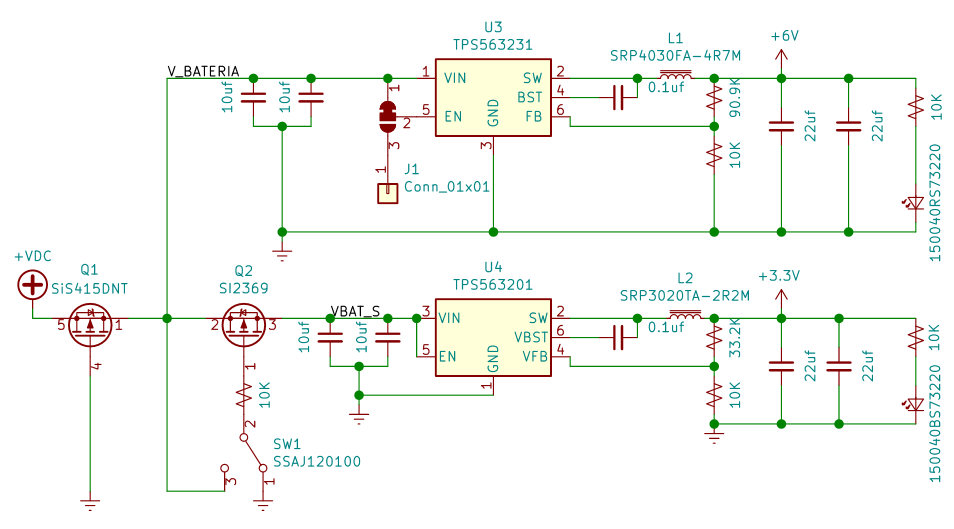
\includegraphics[scale=0.5]{diseniosist/SEn/reguladores.png}  
		\caption{Circuito el�ctrico para regular la tensi�n de $9 [V]$ a $3.3 [V]$ y $6 [V]$. \label{fig:DiagramaRegulacion}}
	\end{center}
\end{figure}

\noindent En la Tabla \ref{tab:ConsumoCansat} se presenta el consumo de energ�a de cada uno de los dispositivos electr�nicos y elementos activos que forman parte del CanSat.

\begin{table}[H]
\begin{center}
\caption{Consumo de energ�a de los dispositivos electr�nicos y elementos activos del CanSat.}
\label{tab:ConsumoCansat}
\resizebox{13cm}{!}{
 \begin{tabular}{p{3cm}c>{\centering}p{2cm}>{\centering}p{1.5cm}>{\centering}p{2cm}>{\centering}p{2.5cm}>{\centering}p{2.5cm}}
\multicolumn{6}{c}{ }\tabularnewline
\toprule

\centering{\textbf{Modelo}} & \textbf{Cantidad} & \textbf{Corriente {[}mA{]}} & \textbf{Voltaje {[}V{]}} & \textbf{Potencia {[}mW{]}} & \textbf{Ciclo de trabajo {[}\%{]}} & \textbf{Fuente de informaci�n}\tabularnewline \hline \tabularnewline

DPS310 & 1 & 0.345 & 3.3 & 1.1385 & 100 & \textit{Datasheet}\tabularnewline
Motorreductor Pololu 50:1 & 2 & 140 & 6 & 648 & 15 & \textit{Datasheet}\tabularnewline
Motorreductor Pololu 380:1 & 1 & 70 & 6 & 2160 & 100 & \textit{Datasheet}\tabularnewline
ICM20948 & 1 & 3.0 & 3.3 & 21.21 & 100 & \textit{Datasheet}\tabularnewline
STM32L432KC & 1 & 6 & 3.3 & 330 & 100 & \textit{Datasheet}\tabularnewline 
STM32F446RE & 1 & 7.2 & 3.3 & 23.76 & 100 & \textit{Datasheet}\tabularnewline
Memoria $\mu$SD & 1 & 100 & 3.3 & 330 & 100& \textit{Datasheet}\tabularnewline
GPS BN180 & 1 & 50 & 3.3 & 165 & 100& \textit{Datasheet}\tabularnewline
Radio XBEE 09P & 1 & 120 & 3.3 & 693 & 100 & \textit{Datasheet}\tabularnewline
CMT-8540S-SMT & 1 & 150 & 6 & 90 & 10 & \textit{Datasheet}\tabularnewline

\bottomrule
\end{tabular}
}
\end{center}
\end{table}

\noindent Las carecter�sticas de la bater�as seleccionadas para ser utilizadas en el CanSat se presentan en la Tabla \ref{BateriasVe}. 

\begin{table}[H]
\begin{center}
\caption{Bater�as consideradas para el veh�culo cient�fico.}
\label{BateriasVe}
\resizebox{15.0cm}{!}{
\begin{tabular}{p{4.0cm}c>{\centering}p{2.5cm}>{\centering}p{2cm}>{\centering}p{1cm}>{\centering}p{4cm}>{\centering}p{2.5cm}}
\multicolumn{6}{c}{}\tabularnewline
\toprule

\centering{\textbf{Modelo}} & \textbf{Composici�n qu�mica} & \textbf{Voltaje nominal {[}V{]}} & \textbf{Capacidad {[}mAh{]}} & \textbf{Masa {[}g{]}} & \textbf{Temperatura de funcionamiento} & \textbf{Fuente de informaci�n}\tabularnewline \hline \tabularnewline

SR44 & Zinc / 
�xido de plata monovalente &  1.55 & 190 & 2.30 & $0^{o} $  a  $70^{o}$& \textit{Datasheet}\tabularnewline

ER 14505 & Cloruro de litio - tionilo &  3.6 & 2600 & 19.0 & $-55^{o}$  a  $85^{o}$& \textit{Datasheet}\tabularnewline

CR2032 &
Litio - di�xido de manganeso
&  3.0 & 230 & 3.0 & $-20^{o}$  a  $70^{o}$& \textit{Datasheet}\tabularnewline

ENERGIZER L522 & Litio - di�xido de manganeso &  9.0 & 1000 & 33.9 & $-40^{o}$  a $60^{o}$& \textit{Datasheet}\tabularnewline
\bottomrule
\end{tabular}
}
\end{center}
\end{table} 

El consumo total de corriente del CanSat en el momento en que todos los elementos est�n trabajando simult�neamente es de $646.545 [mA]$, por lo tanto, se seleccion� la bater�a ENERGIZER L522. La cantidad de corriente que puede generar esta bater�a es de $1000 [mAh]$, adem�s de que el voltaje nominal de $9 [V]$ puede accionar los motores el�ctricos de $6 [V]$ en los sistemas que son utilizados.\\ 

\newpage		
		\subsection{Sistema Estructural} \label{sistSEs}
De acuerdo con la definici�n de la arquitectura f�sica del CanSat, el sistema estructural se encarga de proteger al sistema mecatr�nico de fuerzas internas y externas a las que es sometido, adem�s, permite la conexi�n f�sica y la integraci�n de los otros sistemas y subsistemas.\\

\noindent La figura \ref{fig:SeccionesCanSat} muestra las dos secciones de las que se compone el CanSat: a la izquierda se muestra el contenedor y a la derecha el veh�culo cient�fico.

\begin{figure}[H]
	\centering
		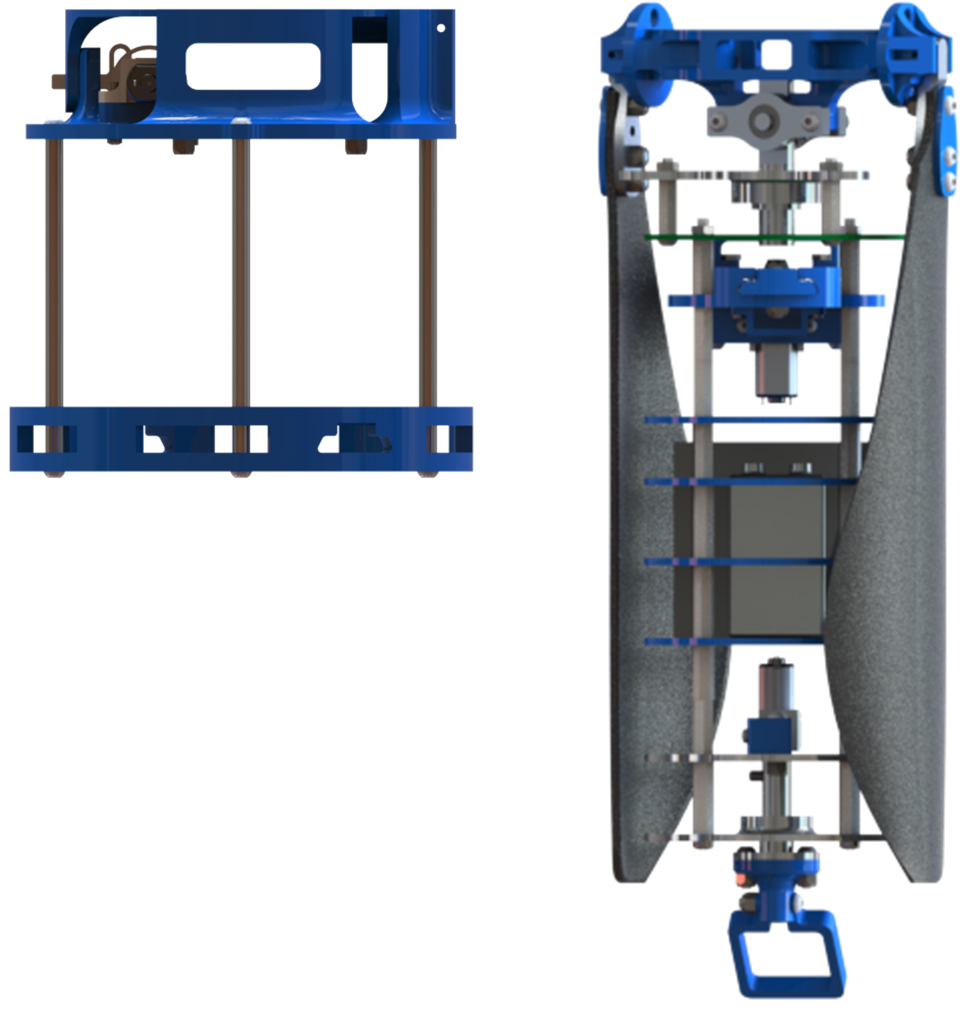
\includegraphics[scale=0.22]{imgmeca/EstructuraCansat.png}
	\caption{Contenedor (izquierda) y veh�culo cient�fico (derecha). 	\label{fig:SeccionesCanSat}}
\end{figure}

\noindent El veh�culo cient�fico estar� dentro del contenedor durante toda la etapa de ascenso, para que despu�s se desacople del contenedor por medio del SLVC.\\

\noindent En la parte superior de la estructura del contenedor se aloja el SRV-P junto con el  mecanismo de apertura del paraca�das. El SRV-P se comunica con la placa principal por medio de dos cables que energizan el motor del mecanismo de apertura del paraca�das.\\

Para las columnas utilizadas en la estructura del contenedor se consider� una cuerda UNF ya que el hilo de las rocas UNF tiene un di�metro mayor que el de las roscas UNC, lo que proporciona a los sujetadores con rosca UNF una resistencia de carga ligeramente mayor y mejores capacidades de bloqueo de torque que los sujetadores con rosca UNC del mismo material (aluminio, en este caso). Adem�s, un �ngulo de avance m�s peque�o permite un ajuste m�s fino a la tensi�n. Las rocas UNF son las m�s ampliamente usadas en la industria aeroespacial.\\

Para que las columnas sean lo m�s ligeras y resistentes posible se utiliz� un tubo redondo extruido con un di�metro exterior de $3/16 [in]$ y espesor de pared de $0.049 [in]$, dejando un di�metro interno de $2.2733 [mm]$ lo que permite hacer una rosca UNF 4-48, o bien, una equivalente ligeramente superior en el sistema m�trico, es decir, una cuerda para tornillo M3. En la figura \ref{img:estructuracontenedor} se presenta la aplicaci�n de las columnas de aluminio.

\begin{figure}[H]
	\centering
		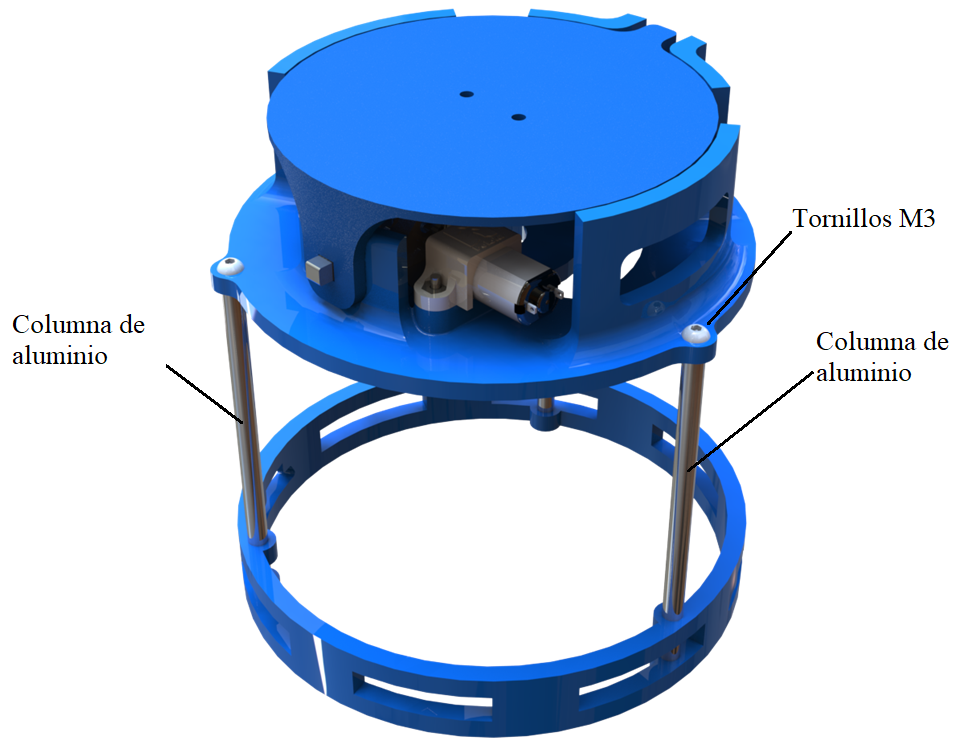
\includegraphics[scale=0.35]{imgmeca/Estructuracontenedor.png}
	\caption{Contenedor del Cansat. 	\label{img:estructuracontenedor}}
\end{figure}

Puesto que el las piezas que conforman el veh�culo cient�fico y el contenedor estar�n expuestas a condiciones de humedad y calor se utilizaron tornillos de acero inoxidable 304 con la finalidad de evitar que las condiciones ambientales afecten la uni�n entre las piezas.\\

Se utilizaron tornillos DIN-7380 puesto que son tornillos que ofrecen un buen apriete en espacios reducidos y son resistentes a la corrosi�n.

\subsection*{Tapa de paraca�das}
Uno de los elementos cr�ticos durante el inicio de la misi�n es la tapa, ya que de este elemento ser� sujetado el Cansat por medio de un gancho al dron con la finalidad de elevarlo a una altura de 400 [m] con respecto del nivel de lanzamiento. Para poder validar que las dimensiones y geometr�as de la tapa ser�n capaces de soportar la carga se realiz� un an�lisis est�tico de esfuerzos y deformaciones por medio del \textit{software} CAD SolidWoks\textsuperscript{\textregistered}. Para esto se hicieron algunas consideraciones. Primeramente, se definieron los puntos en donde la tapa se encontrar� fija, los cuales corresponden al punto en donde se encuentra el eje, el mismo que realiza la funci�n de una bisagra de la tapa, y el punto en donde la tapa estar� sujetada por la corredera del mecanismo de apertura de paraca�das.\\

Para la simulaci�n se consider� que la �nica fuerza que act�a sobre la tapa es el peso del Cansat $\overrightarrow{\text{F}}_{\text{YR}}$, la cual tiene una magnitud de $4.905 [N]$ (considerando una masa de $0.500 [kg]$) y que act�a de manera normal al plano de la tapa. La fuerza $\overrightarrow{\text{F}}_{\text{YR}}$ se divide en dos componentes, $\overrightarrow{\text{F}}_{\text{Y1}}$ y $\overrightarrow{\text{F}}_{\text{Y2}}$, y cada una tendr� la misma direcci�n y la misma magnitud de $2.4525 [N]$, siendo estas dos �ltimas fuerzas las consideradas para la simulaci�n de esfuerzos y deformaciones. Estas fuerzas se muestran en la imagen \ref{img:fuerzastapa}.\\

\begin{figure}[H]
	\centering
		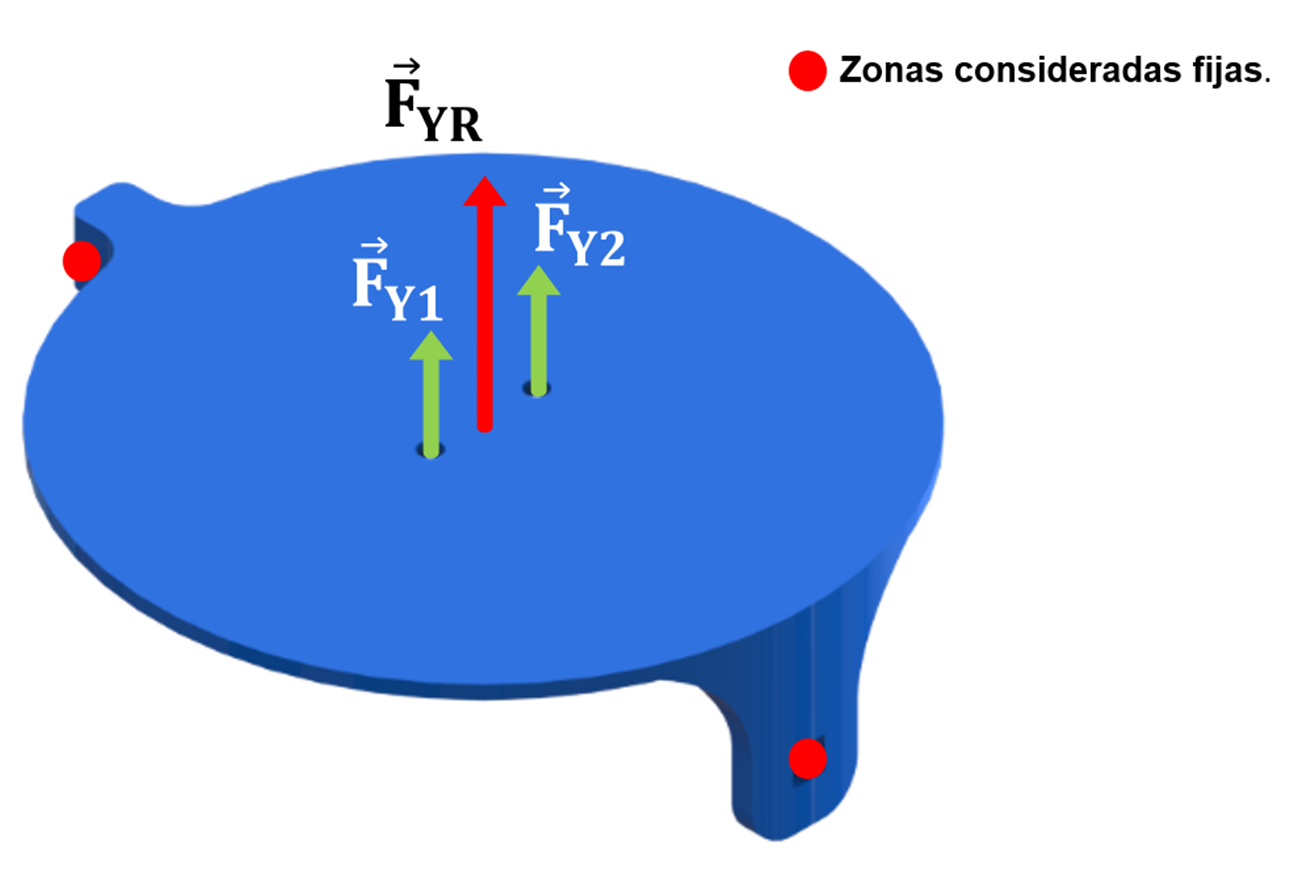
\includegraphics[scale=0.26]{imgmeca/Fuerzasparacaidasdos.png}
	\caption{Fuerzas que act�an en la tapa del contenedor durante el ascenso.\label{img:fuerzastapa}}
\end{figure}

Al realizar una simulaci�n de esfuerzos y deformaciones con el valor de la fuerza previamente calculado se obtienen los siguientes resultados. En \ref{img:simulacionparacaidasuno} se observan los esfuerzos a los que estar� sometida la tapa del paraca�das durente el ascenso del Cansat, siendo el esfuero m�ximo de $3.712 [MPa]$. Este valor de esfuerzo corresponde a un factor de seguridad de 10.50.\\

En la figura \ref{img:simulacionparacaidasdos} se pueden observar las zonas en las que existe un desplazamiento de la estructura de la tapa del paraca�das teniendo una deformaci�n, con respecto a su geoemetria inicial, de $0.09 [mm]$. \newpage

\begin{figure}[H]
	\centering
		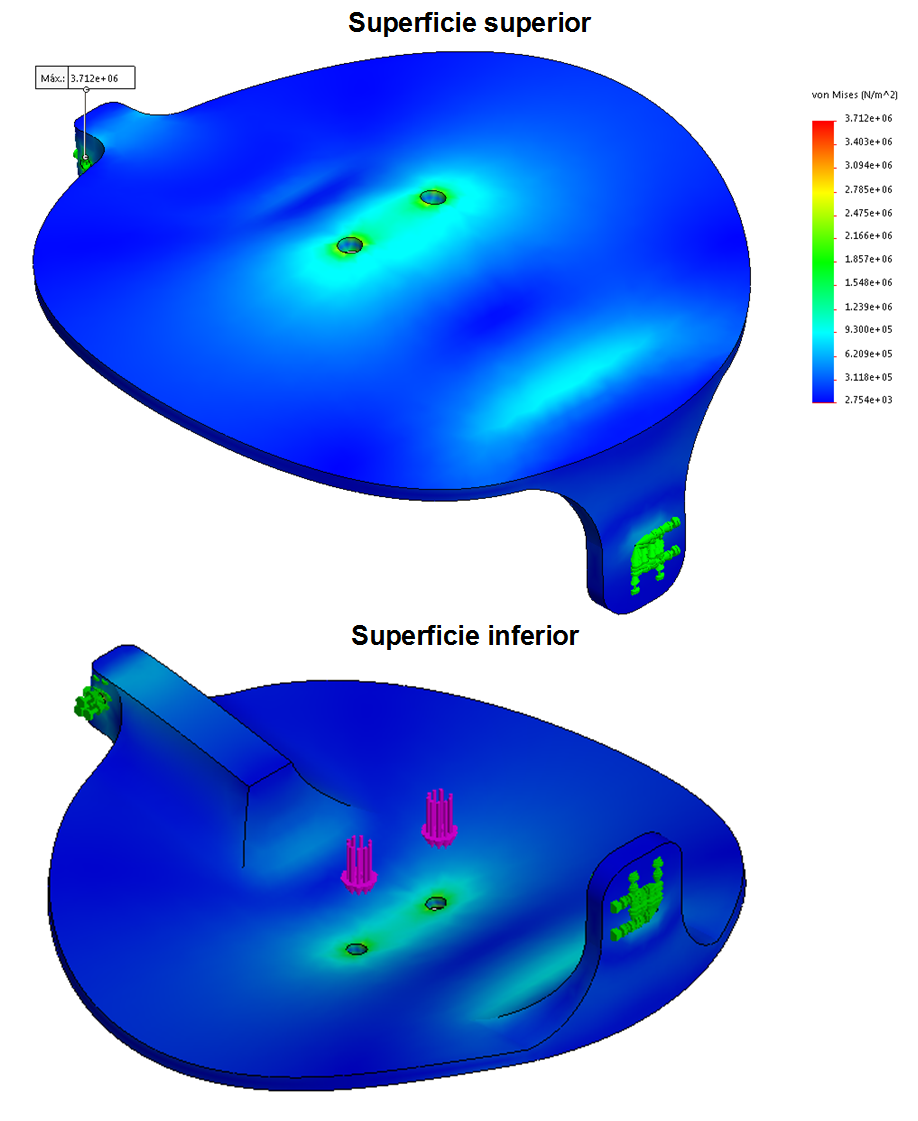
\includegraphics[scale=0.30]{imgmeca/Simulacionparacaidasuno.png}
	\caption{Esfuerzos presentes en la tapa del contenedor durante el ascenso del CanSat. 	\label{img:simulacionparacaidasuno}}
\end{figure}

\begin{figure}[H]
	\centering
		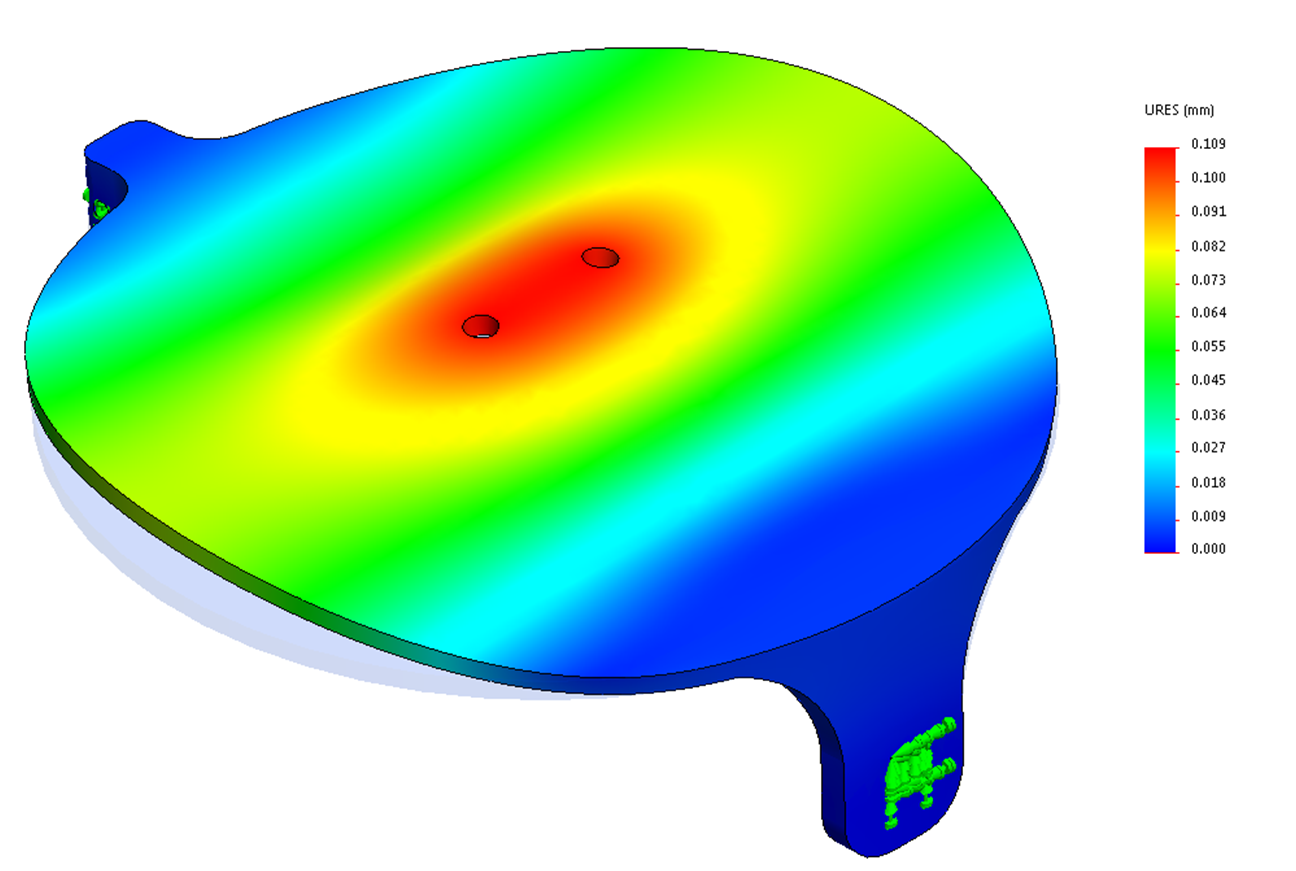
\includegraphics[scale=0.20]{imgmeca/Simulacionparacaidasdos.png}
	\caption{Deformaciones presentes en la tapa del contenedor durante el ascenso del CanSat. 	\label{img:simulacionparacaidasdos}}
\end{figure}

\noindent Otro an�lisis a realizar es el que corresponde al de esfuerzos y deformaciones presentes en la base principal de la secci�n superior del contenedor al momento de desplegar el paraca�das. Este evento ejercer� un tir�n repentino en la base principal de la secci�n superior del contenedor de hasta $30 [Gs]$, lo que equivale a una fuerza $\overrightarrow{\text{F}}$ de $147 [N]$ (tomando un valor de $0.500 [kg]$ para la masa total del CanSat).\\

\noindent La fuerza $\overrightarrow{\text{F}}$ se distribuy� equitativamente en 3 puntos de izaje, como se muestra en la figura \ref{fig:FuerzasOrejas}.

\begin{figure}[H]
	\centering
		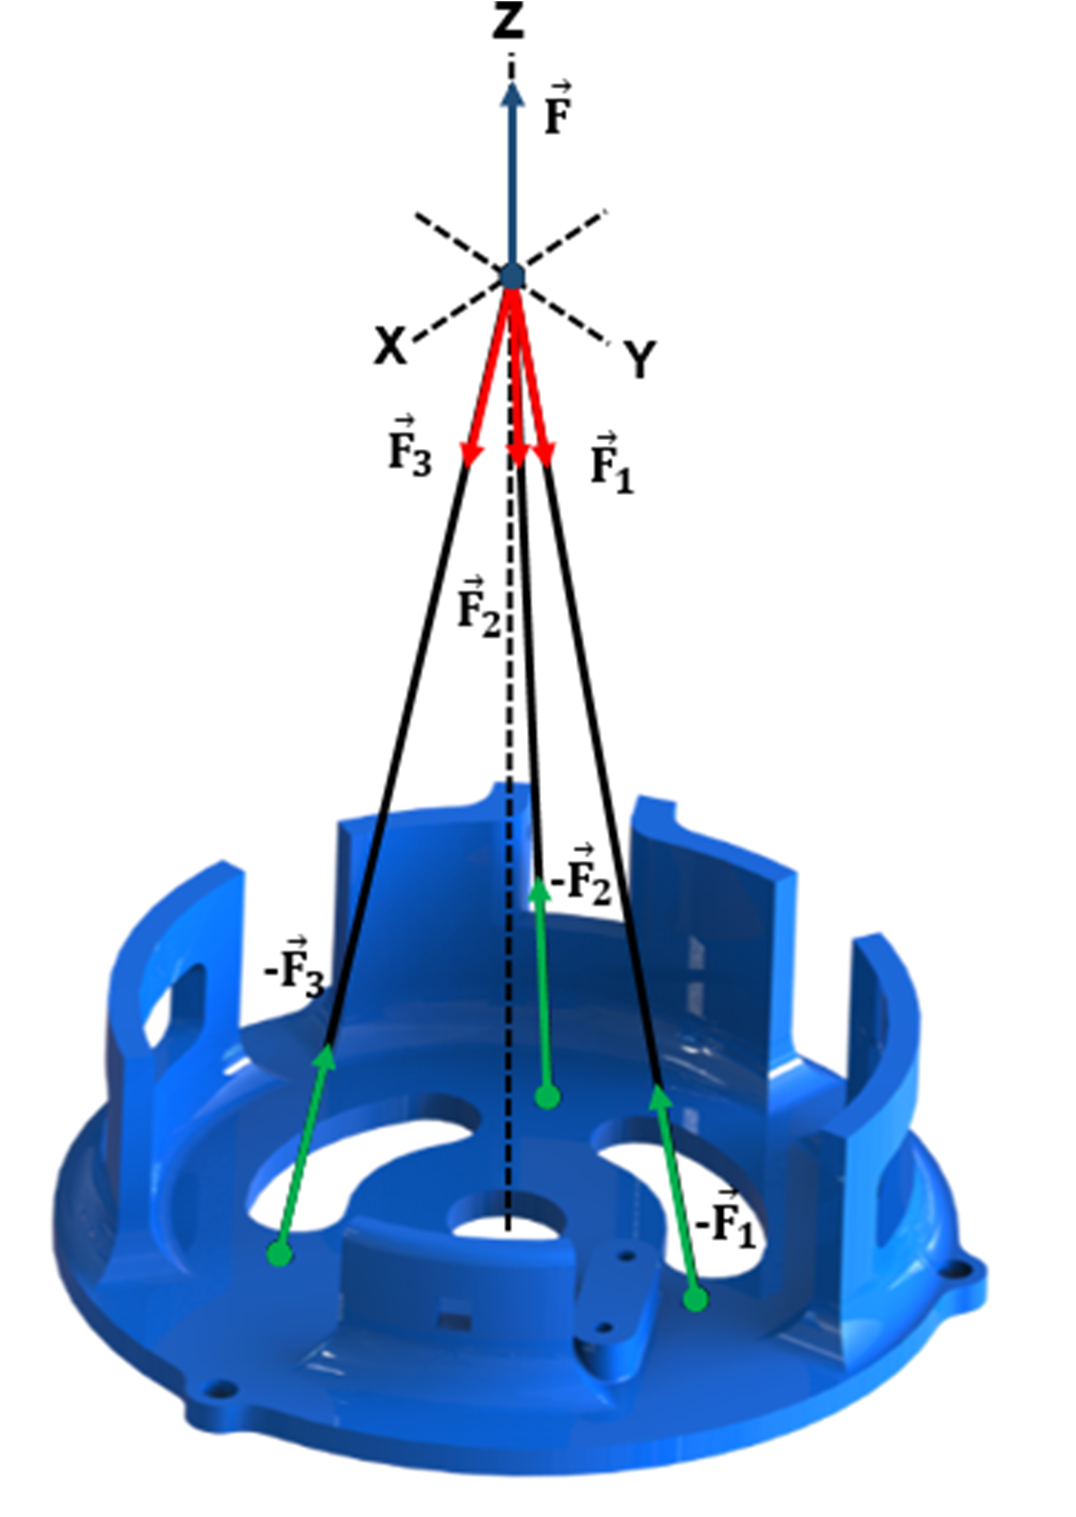
\includegraphics[scale=0.20]{imgmeca/Fuerzasapertura.png}
	\caption{Fuerzas presentes en la base principal del contenedor debidas a la apertura del paraca�das.\label{fig:FuerzasOrejas}}
\end{figure}

\noindent El �ngulo $\theta$ de las fuerzas $\overrightarrow{\text{F}}_{\text{1}}$, $\overrightarrow{\text{F}}_{\text{2}}$ y $\overrightarrow{\text{F}}_{\text{3}}$ es de 70� con respecto del plano $xy$. Es de inter�s calcular la magnitud de cada una de estas fuerzas para poder realizar las simulaciones correspondientes. Con respecto al sistema de referencia mostrado en la figura \ref{fig:FuerzasOrejas}, se tiene que las fuerzas est�n definidas como:\\

$$\overrightarrow{\text{F}}_{\text{1}}=(\text{F}_1 \cos(\theta),0,-\text{F}_1 \sin(\theta))$$
$$\overrightarrow{\text{F}}_{\text{2}}=(-\text{F}_2 \cos(\theta)\cos(\pi/3),\text{F}_2 \cos(\theta) \sin(\pi/3),-\text{F}_2 \sin(\theta))$$
$$\overrightarrow{\text{F}}_{\text{3}}=(-\text{F}_3 \cos(\theta)\cos(\pi/3),-\text{F}_3 \cos(\theta) \sin(\pi/3),-\text{F}_3 \sin(\theta))$$
\newline
\noindent Suponiendo que el sistema se encuentra en equilibrio, se tiene el siguiente sistema de ecuaciones lineal:

\begin{eqnarray}
\left[\begin{array}{ccc}
$$\cos(\theta)$$ & $$-\cos(\theta)\cos(\pi/3)$$ & $$-\cos(\theta)\cos(\pi/3)$$\\
$$0$$ & $$\cos(\theta)\sin(\pi/3)$$ & $$-\cos(\theta)\sin(\pi/3)$$\\
$$-\sin(\theta)$$ & $$-\sin(\theta)$$ & $$-\sin(\theta)$$\\
\end{array} \right]
\left[\begin{array}{ccc}
$$\text{F}_1$$\\
$$\text{F}_2$$\\
$$\text{F}_3$$\\
\end{array} \right]=
\left[\begin{array}{ccc}
$$0$$\\
$$0$$\\
$$F$$\\
\end{array} \right]
\end{eqnarray}

\noindent Cuya soluci�n es:

\begin{eqnarray}
\left[\begin{array}{ccc}
$$\text{F}_1$$\\
$$\text{F}_2$$\\
$$\text{F}_3$$\\
\end{array} \right]=
\left[\begin{array}{ccc}
$$-52.68$$\\
$$-52.68$$\\
$$-52.68$$\\
\end{array} \right]
\end{eqnarray}

\noindent Por lo que $52.68 [N]$ ser� la fuerza que cada punto de izaje deber� soportar. La figura \ref{fig:Baseparacaidasuno} muestra los resultados del an�lisis de esfuerzos respectivo, y la figura \ref{fig:Baseparacaidasdos} los resultados del an�lisis de deformaciones. En esta simulaci�n se establecieron como geometr�a fija los tres puntos de acoplamiento de la secci�n superior del contenedor.\\

\begin{figure}[H]
\begin{center}
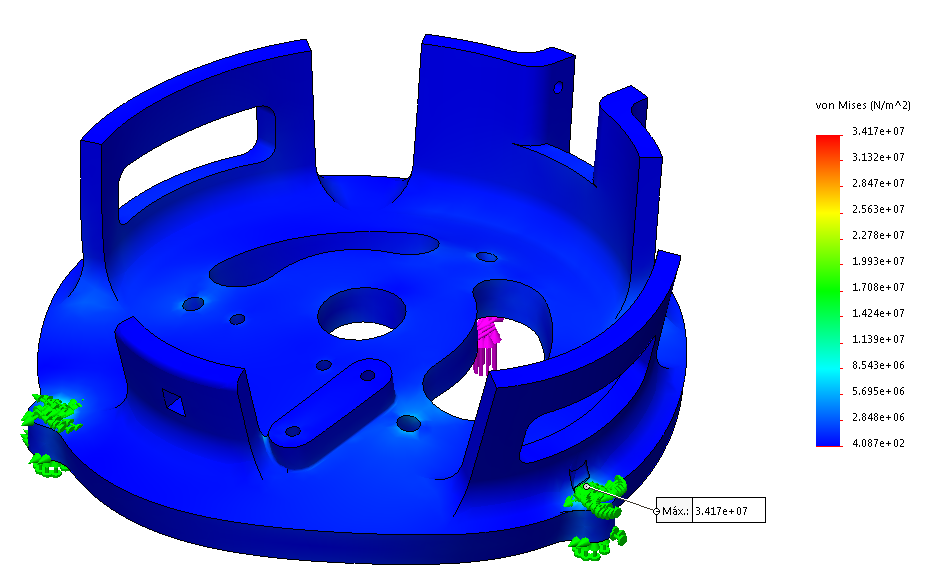
\includegraphics[scale=0.30]{imgmeca/Baseparacaidasuno.png}  
\caption{\label{fig:Baseparacaidasuno}Esfuerzos causados por la apertura del paraca�das en la secci�n superior del contenedor.}
\end{center}
\end{figure}

\begin{figure}[H]
\begin{center}
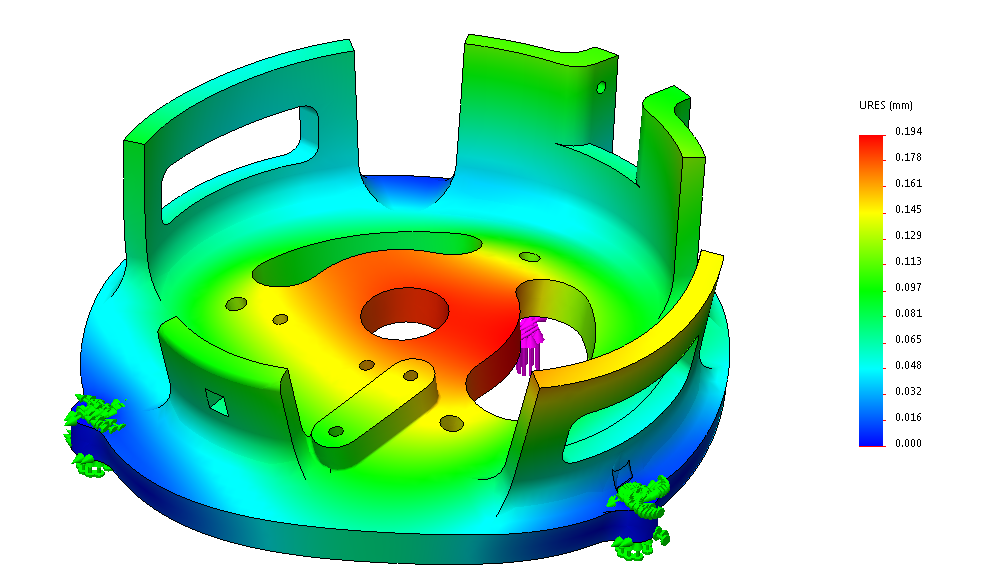
\includegraphics[scale=0.30]{imgmeca/Baseparacaidasdos.png}  
\caption{\label{fig:Baseparacaidasdos}Deformaciones causadas por la apertura del paraca�das en la secci�n superior del contenedor.}
\end{center}
\end{figure}

Para realizar las simulaciones cada una de las fuerzas se descompuso en sus componentes, lo que di� una fuerza vertical de $49.50 [N]$, y una fuerza horizontal, apuntando hacia el centro, de $18.017 [N]$.\\

El esfuerzo m�ximo al que est� sometida la base es de $34.17 [MPa]$ que corresponde con un factor de seguridad de 1.14 que, al estar por encima de la unidad, se considera aceptable.\\

\noindent La estructura del veh�culo cient�fico est� compuesta por varios niveles, todos unidos entre s� por medio de las columnas de soporte de nylon \textit{stand-offs}. El primer nivel corresponde a la base principal del SRV-A. En el segundo nivel est� la placa de circuito principal del SCMC y del SPD. En el tercer nivel se encuentra el SLVC. En el cuarto nivel est� la bater�a y la antena puestos verticalmente. En este nivel tambi�n se encuentra el Xbee y el GPS. Finalmente, acoplado al nivel de la bater�a y la antena, se encuentra el SRD. El interruptor y el LED indicador se ubican en una zona de f�cil acceso y visualizaci�n en la placa de circuito principal. Estos niveles se muestran en la figura \ref{fig:NivelesCansat}.

\begin{figure}[H]
	\begin{center}
		\includegraphics[scale=0.30]{imgmeca/NivelesCansat.png}  
		\caption{\label{fig:NivelesCansat}Niveles del veh�culo cient�fico.}
	\end{center}
\end{figure}

En el veh�culo cient�fico el elemento que est� sometido a mayor esfuerzo es el mecanismo del SLVC. Durante el ascenso las correderas son los elementos que permiten sujetar al veh�culo cient�fico al contenedor hasta el momento en el que el veh�culo cient�fico es  liberado. En \ref{img:simulacioncorredera} se pueden observar las principales fuerzas que est�n presentes en el mecanismo del SLVC al momento del ascenso, en donde $\overrightarrow{\text{F}}_{\text{C1}}$ y $\overrightarrow{\text{F}}_{\text{C2}}$ son las fuerzas que est�n presentes en cada una de las correderas, cuyo valor es de $1.962 [N]$ (considerando una masa de $0.4 [kg]$ para el veh�culo cient�fico). 

\begin{figure}[H]
	\centering
		\includegraphics[scale=0.26]{imgmeca/Simulacioncorredera.png}
	\caption{Fuerzas asociadas al mecanismo de liberaci�n durante el ascenso.	\label{img:simulacioncorredera}}
\end{figure}

Cuando el veh�culo cientif�co est� en ascenso la fuerza se trasnmite a la base principal del SLVC, por lo que es �sta la que recibe el esfuerzo. De acuerdo con la figura \ref{img:simulacioncorrederauno} el esfuerzo m�ximo en la base principal del SLVC es de $4.072 [MPa]$ y, por lo tanto, se puede determinar que el factor de seguridad es de 9.57.

 \begin{figure}[H]
	\centering
		\includegraphics[scale=0.26]{imgmeca/Simulacioncorrederauno.png}
	\caption{Esfuerzos presentes en la base principal del SLVC.	\label{img:simulacioncorrederauno}}
\end{figure}

En la figura \ref{img:simulacioncorrederados} se presentan las zonas de desplazamiento de la base principal del SLVC en donde se observa que la deformaci�n m�xima es menor a un milimetro.

 \begin{figure}[H]
	\centering
		\includegraphics[scale=0.26]{imgmeca/Simulacioncorrederados.png}
	\caption{Deformaciones presentes en la base principal del SLVC.	\label{img:simulacioncorrederados}}
\end{figure}

	
\newpage
		\subsection{Integraci�n del Sistema Mecatr�nico} \label{sistIntegracion}
La figura \ref{img:CanSatconstruido} muestra el CanSat completo construido y ensamblado con se�alizaci�n a las partes de mayor nivel.

\begin{figure}[H]
	\centering
	\includegraphics[scale=0.40]{Resultados/integracion.png}
	\caption{CanSat ensamblado.}
	\label{img:CanSatconstruido}
\end{figure}

\noindent Las figuras \ref{img:placatop} y \ref{img:placabottom} muestran la cara superior y la cara inferior de la placa de circuito principal, respectivamente.

\begin{figure}[H]
	\centering
	\includegraphics[scale=0.23]{implementacion/SCMCySPD/reservas/PlacaTop.png}
	\caption{Cara superior de la placa de circuito principal.}
	\label{img:placatop}
\end{figure}

\begin{figure}[H]
	\centering
	\includegraphics[scale=0.30]{implementacion/SCMCySPD/reservas/PlacaBottom.png}
	\caption{Cara inferior de la placa de circuito principal.}
	\label{img:placabottom}
\end{figure}